\documentclass[11pt]{article}
\usepackage{debulletin,times,epsfig,subfigure,wrapfig,algorithmic,color,boxedminipage,graphicx,url}

% this is the template for an issue of the Data Engineering Bulletin

% all packages used by any paper must be listed here
\usepackage{subfig}
\usepackage{listings}
\usepackage{caption}
\usepackage{microtype}
\usepackage{listings}
\usepackage{booktabs}
\usepackage{listings}
\usepackage{xargs}
\usepackage{amsmath, amssymb}
\usepackage{enumitem}

%% Zick
\usepackage[ruled,linesnumbered]{algorithm2e}
\DeclareMathOperator{\argmin}{\mathrm{argmin}}
\DeclareMathOperator{\loc}{\mathit{loc}}
\DeclareMathOperator{\Dist}{\mathit{Dist}}
\DeclareMathOperator{\Ethn}{\mathit{Type}}
\DeclareMathOperator{\Proj}{\mathit{Project}}
\DeclareMathOperator{\Price}{\mathit{Price}}
\DeclareMathOperator{\UB}{\mathit{UB}}
\DeclareMathOperator{\LB}{\mathit{LB}}


%\PassOptionsToPackage{hyphens}{url}
%\usepackage{hyperref}
\usepackage{multirow}
\usepackage{tabularx}
\usepackage{makecell}
\usepackage{arydshln}
\usepackage{xspace}
\usepackage{tcolorbox}
\usepackage{xpatch}

\newcommand{\Hypercallback}{Hyperupcall\xspace{}}
\newcommand{\hypercallback}{hyperupcall\xspace{}}
\newcommand{\hide}[1]{}

% Added to remove warning from Salimi's article
\pdfminorversion=7


\begin{document}


% please enter real date, vol no, issue no
\bulletindate{September 2019}
\bulletinvolume{42}
\bulletinnumber{3}
\bulletinyear{2019}

% these are files that I have- but your part of the issue can be done without
% them
\IEEElogo{cs.pdf}
\insidefrontcover{incvA19.pdf}
%\insidebackcover[ICDE Conference]{./calls/icde-new-a.ps}

\begin{bulletin}

% the above samples assume the issue is generated from a directory structure of the following sort
% major directory name is month and year of issue
% there are sub-directorys for
% letters: directory name is "letters"
% technical articles: a directory per paper, named for an "author"
% news articles: directory name is "news"
% calls: directory name is "calls

%
%  Editor letters section.  Use the lettersection environment.
%  Each letter is contained in a letter environment, where the two required
%  options to \begin{letter} are the author and the address of the author.
%

\begin{lettersection}

% there will be other letters- and a blank page will appear in your document
% but the special issue part will be fine

\begin{letter}{Letter from the Editor-in-Chief}
{Haixun Wang}{WeWork Corporation}
\documentclass[11pt]{article} 

\usepackage{deauthor,times,graphicx}
%\usepackage{url}
\usepackage{hyperref}

\begin{document}
Around the time we published our last issue in March, the nation went
into a lockdown. Life in the last 3 months has been unprecedented in
many ways. As governments around the world scrambled to fight
coronavirus, people in the scientific community, especially those on
the frontline -- doctors, healthcare professionals, medical staff and
researchers -- made heroic efforts and sacrifices to curb the pandemic
and save lives. The data management and data science communities also
sprang to action immediately. Globally, it is the first time that data
driven approaches are being used at such a large scale toward solving
a common problem. Under this backdrop, in this special issue of the
Data Engineering Bulletin edited by Joseph Gonzalez, we feature 8
papers on the topic of {\it digital contact tracing}, a technique that
may prove crucial in the fight against Covid-19.

This issue also features two opinion pieces. Divyakant Agrawal and Amr
El Abbadi's wake-up call on managing data in an untrusted environment
takes us to the fascinating world of cryptocurrencies and
blockchains. It shows what the database community, which was
responsible for creating and perfecting transaction management and
distributed systems, can learn from the blockchain approach when it
comes to handling untrusted behaviours from the underlying
infrastructure. The second opinion piece, written by Jeffrey
D. Ullman, addresses a question on the mind of every data management
person: What is our role in the machine learning and AI revolution?
Have we missed the boat again and become irrelevant? Ullman's
perspective, illustrated by his remake of the well known Conway Venn
Diagram that illustrates the relationship between computer science,
mathematics \& statistics, and domain knowledge is incisive,
thought-provoking, and entertaining at the same time.
\end{document}


\end{letter}
%
\newpage
%
%% your introductory letter goes here

\begin{letter}{Letter from the TCDE Awards Committee Chair}
{Johannes Gehrke}{Microsoft, USA}
%\documentclass[11pt,dvipdfm]{article}
%\usepackage[utf8]{inputenc}

%\title{The 2019 IEEE TCDE Awards}
%\author{2019 IEEE TCDE Awards Committee}
%\date{September 2019}

%\begin{document}
%\maketitle

%\vspace{-0.1in}

The IEEE TCDE (Technical Committee of Data Engineering) has established several highly prestigious awards to encourage innovative long term contributions to the field of data engineering. It is our pleasure to present letters from the 2019 award winners in this issue.

%\begin{itemize}

%\item 
\  
\\
{\bf Rising Star Award.} The IEEE TCDE Rising Star Award is based on an individual's whole body of work in the first five years after the PhD. The award aims to promote current database researchers as they create their career. The 2019 IEEE TCDE Rising Star Award goes to Viktor Leis from the Technical University of Munich
for \emph{contributions to main-memory indexing and database architectures for NVM}.

%\item 
\  
\\
{\bf Impact Award.} The IEEE TCDE Impact Award recognizes database researchers whose research resulted in impact beyond the data engineering field, impact beyond research to industrial practice, and/or impact resulting in expansion of the data engineering field itself. The 2019 IEEE TCDE Impact Award goes to 
Christian Jensen from Aalborg University for \emph{contributions to spatial, temporal, and spatio-temporal data management}.

%\item 
\  
\\
{\bf Service Award.} The IEEE TCDE Service Award recognizes an individual who has contributed significantly to ICDE, TCDE, and the data engineering community in general. The 2019 IEEE TCDE Service Award goes to David Lomet from Microsoft for 
\emph{leadership as the Editor-in-Chief of the Data Engineering Bulletin for over 25 years}.\\
%\end{itemize}
\indent
\ 
\\
Congratulations again to the winners, and we hope you will enjoy reading their letters as much as we did.

%\newline
\vspace{0.1in}

\begin{flushright}
\indent {\bf The 2019 Awards Committee} \\
%\vspace{ex} \\
%\vspace{0.1in} \\
\indent Anastasia Ailamaki\\
\indent Paolo Atzeni\\
\indent Michael Carey \\
\indent Xin Luna Dong \\
\indent Johannes Gehrke (chair) \\
\indent Sunita Sarawagi
\end{flushright}
% \end{document}

\end{letter}

\newpage

\begin{letter}{Letter from the Special Issue Editor}
{Alexandra Meliou}{University of Massachusetts, Amherst}
\documentclass[11pt]{article} 

\usepackage{deauthor,times,graphicx}
%\usepackage{url}
\usepackage{hyperref}



\begin{document}

The big data revolution and advancements in machine learning
technologies have revolutionized decision making, advertising,
medicine, and even election campaigns. Data-driven software now
permeates virtually every aspect of human activity and has the
ability to shape human behavior: it affects the products we view
and purchase, the news articles we read, the social interactions we
engage in, and, ultimately, the opinions we form. Yet, data is an
imperfect medium, tainted by errors, omissions, and biases. As a
result, discrimination shows up in many data-driven applications,
such as advertisements, hotel bookings, image search, and vendor
services. In this issue, we bring together an exciting collection
of recent and ongoing work that focuses on the problems of
fairness, diversity, and transparency in data-driven systems. This
collection highlights the central role that the data management
research community can play in detecting, informing, and mitigating
the effects of bias, skew, and misuse of data, and aims to create
bridges with work in related communities.




\end{document}



\end{letter}

\end{lettersection}



% put the name of your special issue below

\begin{opinionsection}
\begin{opinion}{Value Creation from Massive Data in Transportation -- The Case of\\ Vehicle Routing}
{Christian S. Jensen}{Aalborg University, Denmark}
\documentclass[11pt]{article}
\usepackage{deauthor,times,graphicx}

\begin{document}

% \noindent
% \textbf{\Large Value Creation from Massive Data in Transportation---The Case of Vehicle Routing}
% \newline

% \begin{center}
% Christian S.\ Jensen\\
% Aalborg University  
% \end{center}

%\title{Value Creation from Massive Data in Transportation---The Case of Vehicle Routing}

%\author{Christian S.\ Jensen\\ Aalborg University}

%\maketitle


\section{Introduction}

Vehicular transportation will undergo profound change over the next decades, due to developments such as increasing mobility demands and increasingly autonomous driving. At the same time, rapidly increasing, massive volumes of data that capture the movements of vehicles are becoming available. In this setting, the current vehicle routing paradigm falls short, and we need new data-intensive paradigms. In a data-rich setting, travel costs such as travel time are modeled as time-varying distributions: at a single point in time, the time needed to traverse a road segment is given by a distribution. How can we best build, maintain, and use such distributions? 

The travel cost of a route is obtained by convolving distributions that model the costs of the segments that make up the route. This process is expensive and yields inaccurate results when dependencies exist among the distributions. To avoid these problems, we need a path-centric paradigm, where costs are associated with arbitrary paths in a road network graph, not just with edges. This paradigm thrives on data: more data is expected to improve accuracy, but also efficiency. Next, massive trajectory data makes it possible to compute different travel costs in different contexts, e.g., for different drivers, by using different subsets of trajectories depending on the context. It is then no longer appropriate to assume that costs are available when routing starts; rather, we need an on-the-fly paradigm, where costs can be computed during routing. Key challenges include how to achieve efficiency and accuracy with sparse data. Finally, the above paradigms assume that the benefit, or cost, of a path is quantified. As an alternative, we envision a cost-oblivious paradigm, where the objective is to return routes that match the preferences of local, or expert, drivers without formalizing costs.


\section{Background}

Vehicular transportation is an inherent aspect of society and our lives: many people rely on vehicular transportation on a daily basis, we spend substantial time on transportation, and we are often forced to arrange our lives around traffic. As a reflection of this, society spends very substantial resources on enabling safe, reliable, clean, and inexpensive transportation. Due to a combination of interrelated developments, transportation will undergo profound changes in the years to come.

First, a range of key enabling technologies have reached levels of sophistication that make (semi-)autonomous vehicles possible. For example, Tesla cars already come with an autopilot that is a pre-cursor to autonomous driving, and virtually all major vehicle manufacturers are working to make autonomous cars. The state of affairs is similar to the one that applied to personal computing when Apple and Microsoft were created and the one that applied to the Internet when Google was founded. Second, the sharing economy trend is also gaining traction in relation to vehicular transportation, thus enabling better exploitation of under-utilized vehicles. For example, Uber enables transportation in private vehicles by private drivers. Online ridesharing services such as Lyft enable the sharing of trips. A large number of similar services exist across the globe. Next, other developments such as urbanization and the needs to combat air pollution and greenhouse gas emissions will also impact transportation. Many large cities are facing air quality problems, and the transportation sector is the second largest contributor to GHG emissions, trailing only the energy sector.

These increasingly pressing developments promise a perfect storm for transportation: While it is not clear exactly how this will play out, it is clear that transportation faces profound change. For example, Uber and similar services may eventually do away with under-paid drivers. When a person goes to a movie theater and cannot find parking, the driver may instead let the car serve as a self-driving taxi, thus making money instead of paying money for parking while watching a movie.

We are also witnessing a digitalization trend that is unprecedented in the history of humanity: We are increasingly instrumenting societal and industrial processes with networked sensors. As a result, we are accumulating massive volumes of data that capture the states of processes and that may be used for enabling rational, data-driven processes and data-driven decision making. This also applies to transportation. Vehicles are increasingly online, via smartphones or built-in connectivity, and they are equipped with global navigation satellite system (GNSS) positioning capabilities, e.g., Galileo, GPS, and Glonass, via smartphones or in-vehicle navigation systems. As a result, rapidly increasing volumes of vehicle data are becoming available. This data includes vehicle trajectory data, i.e., sequences of GNSS records that record time and location. This new data source captures transportation at a level of detail never seen before.

With the diffusion of smartphones and in-vehicle navigation devices, routing is now available to a very large fraction of the population on Earth. Indeed, the availability of routing is now taken for granted, and routing is used widely. Further, the advances in autonomous and semi-autonomous vehicles make it a safe bet that more and more routing decisions will be taken by machines using some form of routing service, rather than by people. Thus, the importance of routing will increase over the coming years.

The foundation for traditional routing was built at a time where little data was available. We contend that given the above observations, new foundations are needed to enable routing capable of effectively exploiting available data to enable efficient and accurate, high-resolution routing services.


\section{New Routing Paradigms}

\paragraph{Traditional Routing} The setting that underlies traditional routing services is one where a road network is modeled as a weighted graph and where the weight of an edge captures the cost of traversing the road segment modeled by the edge. In this setting, a graph with real-valued edge weights, capturing, e.g., travel distance, is given and some routing algorithm is applied to identify a route from a source to a destination with the minimum sum of edge weights. More advanced edge weights that capture travel time are also considered. While many different routing algorithms exist for such weighted road-network graphs, the prototypical algorithm is Dijkstra's algorithm \cite{1}; hence, we call this Dijkstra's paradigm. This paradigm is well suited for settings were little travel data is available. Notably, by assigning weights to the atomic paths, i.e., individual graph edges, the paradigm makes the best possible use of available data. However, we contend that this simple edge-centric paradigm is obsolete and hinders progress in settings were travel costs are extracted from trajectories. Dijkstra's paradigm falls short when it comes to exploiting massive volumes of trajectory data for enabling more accurate and higher-resolution routing.

Given a (source, destination)-pair and a departure time, a typical routing service computes one or more paths from the source to the destination with the fastest travel time as of the departure time. ``High resolution'' implies that travel times in a road network are modeled (i) at a fine temporal granularity, as traffic changes continuously and affects travel time, and (ii) as distributions, as different drivers may have different travel times even when driving on the same path at the same time, and as traffic is inherently unpredictable. Further high resolution implies that routing takes into account the particular context, e.g., the driver, yielding personalized routing, or weather conditions \cite{2,3,4}.

We envision three new routing paradigms that are capable of exploiting massive trajectory data to enable more accurate and higher-resolution routing services.

\paragraph{Path-centric paradigm} In this paradigm, costs are associated with arbitrary paths in a road network graph, rather than just with edges. This avoids unnecessary fragmentation of trajectories and automatically enables detailed capture of dependencies as well as turning and waiting times at intersections. This paradigm thrives on data: the more trajectory data, the better the accuracy and resolution of the routing. Further, more data also promises more efficient routing, which is less intuitive. With this paradigm, the cost, e.g., travel time, of an arbitrary path is estimated from available costs of paths that intersect the path. Fewer costs have to be assembled than in the edge-centric paradigm. For example, with costs being probability distributions and a path containing 100 edges, convolution must be applied 99 times to assemble 100 distributions into one in Dijkstra's paradigm. With sufficient trajectory data, a path may be covered by a few long paths with costs in the path-centric paradigm. Thus, computing the path's cost will require only a few convolutions. Thus, this paradigm holds the potential to enable more efficient routing the more trajectory data that is available. In the extreme, computing the cost of an arbitrary path can be achieved by means of a lookup, with no need for convolution. Next, when using Dijkstra's algorithm, intuitively, when a search has reached a graph vertex, the lowest-cost path to reach that vertex is known and fixed; thus, all other paths for reaching the vertex can be disregarded, or pruned. In the new paradigm, the cost of reaching a vertex can change when the search proceeds from the vertex because a different set of path costs that reach into the past may be used. It may happen that the cost of the path used for reaching the vertex increases and that a lower-cost path now exists.

In the path centric-paradigm, the underlying data structure is no longer just a graph, as path weights need to be maintained, and the correctness of Dijkstra's algorithm is no longer guaranteed. In initial work \cite{5,6}, we have taken first steps to define and explore some aspects of the path-centric paradigm. These studies confirm that the paradigm holds substantial promise and is ``the right'' paradigm when massive trajectory data is available.

\paragraph{On-the-fly paradigm} Next, massive trajectory data makes it possible to compute different travel costs in different contexts, e.g., for different drivers, by using different subsets of trajectories depending on the context. In this setting, it is no longer appropriate to assume that precomputed costs are available when routing starts, which is the standard assumption. There are simply too many costs to compute and store, most of which will never be used. Instead, we need an on-the-fly paradigm, where costs can be computed during routing. When, during routing, we need to determine the cost distribution of an edge or a path, we need to retrieve the relevant parts of the available trajectories that contain useful cost information given the particular context considered. These parts are then used to form an accurate cost distribution. The retrieval task takes a path, the time-of-arrival at the path, and contextual information such as a user identifier and weather information as arguments. Then the task is to retrieve sub-trajectories that contain information relevant to these arguments. As a routing query should preferably take less than 100 milliseconds, it is very difficult to achieve the necessary efficiency, and indexing techniques are needed that go beyond existing techniques \cite{7,8,9}. Another challenge is to determine which trajectories to actually use when computing the most accurate weight distributions. We have conducted preliminary studies focused on achieving better indexing \cite{91} and understanding the accuracy problem \cite{10,11}. The studies indicate that the challenges are substantial.

\paragraph{Cost-oblivious paradigm} The above paradigms rely on the same underlying assumption as does Dijkstra's paradigm: We use trajectory data for computing costs, and then we apply a routing algorithm to find lowest-cost paths. In essence, these paradigms only use trajectories for extracting costs such as travel time and GHG emissions \cite{12}. However, trajectories contain much more information that could potentially be utilized for achieving better routing: Trajectories tell which routes drivers follow and seemingly prefer. This paradigm is behavioral in the sense that it aims to exploit this route-choice behavior. An earlier study \cite{13} indicates that historical trajectories are better at predicting the route a driver will take from a source to a destination than is the route returned by a cost-based routing service. This study thus confirms that the cost-oblivious paradigm holds potential for enabling better routing. And again, this is a paradigm that is shaped to thrive on data: If enough data is available to cover all (source, destination)-pairs with trajectories, routing could be achieved by means of a lookup, with no need for a travel-cost based routing algorithm. We have already proposed a simple route-recommendation solution and have compared it with existing solutions \cite{14}. These solutions do not contend well with sparse data. In addition, we have proposed a first attempt at making better use of sparse data \cite{15} for path recommendation within this paradigm.

\paragraph{Synergies} It is important to observe that specific routing solutions can be composed of elements from Dijkstra's paradigm and all three new paradigms. For example, a predominantly on-the-fly solution may rely on pre-computed edge weights as a fall-back; and if insufficient data is available to a cost-oblivious solution, some limited form of routing may be applied. Beyond this, the fleshing out of the three paradigms relies on the same experimental infrastructure, encompassing computing capabilities, software pipelines, data, and methodologies. 

\section{Summary}

In a world with more than 2.5 billion smartphone users and about 1 billion cars, and where routing decisions are increasingly being made by machines, the line of research outlined here has the potential for very large societal impact. It literally holds the potential to make a difference for on the order of a billion users. High-quality routing has significant benefits. It can make transportation more predictable, an important property of a transportation system that reduces the need to ``leave early'' and thus the time spent on transportation. In addition, it may increase the capacity of an existing infrastructure by making each trip more efficient, making room for more trips, and by incentivizing drivers to ``spread out'' their trips, e.g., by quantifying the time saved by traveling before or after rush hour. Routing also holds the potential to reduce the GHG emissions per trip \cite{16,17}. Finally, the above coverage of problems related to the use of massive trajectory data for value creation in transportation is by no means exhaustive. 

\paragraph{Acknowledgments} I would like to thank the many hard-working colleagues with whom I have worked and am working to make progress on the topics described here.

\begin{thebibliography}{15}

\bibitem{1}
E. W. Dijkstra. \emph{A note on two problems in connexion with graphs}. Numer. Math., vol. 1, no. 1, pp. 269--271, 1959.

\bibitem{2}
J. Letchner, J. Krumm and E. Horvitz. \emph{Trip Router with Individualized Preferences (TRIP): Incorporating Personalization into Route Planning}. In AAAI, 2006.

\bibitem{3}
B. Yang, C. Guo, Y. Ma and C. S. Jensen. \emph{Toward personalized, context-aware routing}. VLDB J, vol. 24, no. 2, pp. 297--318, 2015.

\bibitem{4}
O. Andersen and K. Torp. \emph{A Data Model for Determining Weather's Impact on Travel Time}. In DEXA, 2016.

\bibitem{5}
J. Dai, B. Yang, C. Guo, C. S. Jensen and J. Hu. \emph{Path Cost Distribution Estimation Using Trajectory Data}. PVLDB, vol. 10, no. 3, pp. 85--96, 2016.

\bibitem{6}
B. Yang, J. Dai, C. Guo, C. S. Jensen and J. Hu. \emph{PACE: a PAth-CEntric paradigm for stochastic path finding}. VLDB J, vol. 27, no. 2, pp. 153--178, 2018.

\bibitem{7}
B. B. Krogh, N. Pelekis, Y. Theodoridis and K. Torp. \emph{Path-based queries on trajectory data}. In SIGSPATIAL GIS, 2014.

\bibitem{8}
B. B. Krogh, C. S. Jensen and K. Torp. \emph{Efficient in-memory indexing of network-constrained trajectories}. In SIGSPATIAL GIS, 2016.

\bibitem{9}
S. Koide, Y. Tadokoro, C. Xiao and Y. Ishikawa. \emph{CiNCT: Compression and retrieval of massive vehicular trajectories via relative movement labeling}. In ICDE, 2018.

\bibitem{91}
R. Waury, C. S. Jensen, S. Koide, Y. Ishikawa, and C. Xiao. \emph{Indexing Trajectories for Travel-Time Histogram Retrieval}. In EDBT 2019.

\bibitem{10}
R. Waury, J. Hu, B. Yang and C. S. Jensen. \emph{Assessing the Accuracy Benefits of On-the-Fly Trajectory Selection in Fine-Grained Travel-Time Estimation}. In MDM, 2017.

\bibitem{11}
R. Waury, C. S. Jensen and K. Torp. \emph{Adaptive Travel-Time Estimation: A Case for Custom Predicate Selection}. In MDM, 2018.

\bibitem{12}
C. Guo, B. Yang, O. Andersen, C. S. Jensen and K. Torp. \emph{EcoMark 2.0: empowering eco-routing with vehicular environmental models and actual vehicle fuel consumption data} Geoinformatica, vol. 19, no. 3, pp. 567--599, 2015.

\bibitem{13}
V. Ceikute and C. S. Jensen. \emph{Routing Service Quality - Local Driver Behavior Versus Routing Services}. In MDM, 2013.

\bibitem{14}
V. Ceikute and C. S. Jensen. \emph{Vehicle Routing with User-Generated Trajectory Data} In MDM, 2015.

\bibitem{15}
C. Guo, B. Yang, J. Hu and C. S. Jensen. \emph{Learning to Route with Sparse Trajectory Sets}. In  ICDE, 2018.

\bibitem{16}
O. Andersen, C. S. Jensen, K. Torp and B. Yang. \emph{EcoTour: Reducing the Environmental Footprint of Vehicles Using Eco-routes}. In MDM, 2013.

\bibitem{17}
C. Guo, B. Yang, O. Andersen, C. S. Jensen and K. Torp. \emph{EcoSky: Reducing vehicular environmental impact through eco-routing}. In ICDE, 2015.

% \bibitem{reviewER2012} 
% X. Cao, L. Chen, G. Cong, C. S. Jensen, Q. Qu, A. Skovsgaard, D. Wu, and M. L. Yiu. \emph{Spatial Keyword Querying}. In ER, 2012, pp. 16--29.

% \bibitem{lda}
% D. M. Blei, A. Y. Ng, and M. I. Jordan. \emph{Latent dirichlet allocation}. J. Mach. Learn. Res., vol. 3, pp. 993--1022, 2003.

\end{thebibliography}

\end{document}

\end{opinion}
\end{opinionsection}




% \begin{articlesection}{Data Fairness, Diversification, and Responsible Data Management}
\begin{articlesection}{Fairness, Diversity, and Transparency in Data Systems}
%
%  Contributed articles section.  Use the articlesection environment.
%  Each article is contained in an article environment, where the two required
%  options to \begin{article} are the title and author of the article
%
%\begin{article}
%{Title of article}
%{list of authors}
%\input{author-name/article.tex}
%\end{article}


\begin{article}
{Nutritional Labels for Data and Models}
{Julia Stoyanovich, Bill Howe}
\graphicspath{{submissions/Stoyanovich/}}
\pdfminorversion=5
\documentclass[11pt]{article}
\usepackage{deauthor,times,graphicx,caption,microtype}
\usepackage{hyperref}
\usepackage{listings}
\usepackage{booktabs}

\begin{document}

\title{Optimistic Lock Coupling: A Scalable and Efficient General-Purpose Synchronization Method}

\author{Viktor Leis, Michael Haubenschild\raisebox{0.9ex}{$\ast$}, Thomas Neumann\\ Technische Universit{\"a}t M{\"u}nchen \hspace{0.7cm} Tableau Software\raisebox{0.9ex}{$\ast$} \\ {\{leis,neumann\}{@}in.tum.de} \hspace{0.7cm} {mhaubenschild{@}tableau.com\raisebox{0.9ex}{$\ast$}}}

\maketitle

\begin{abstract}
As the number of cores on commodity processors continues to increase, scalability becomes more and more crucial for overall performance.
Scalable and efficient concurrent data structures are particularly important, as these are often the building blocks of parallel algorithms.
Unfortunately, traditional synchronization techniques based on fine-grained locking have been shown to be unscalable on modern multi-core CPUs.
Lock-free data structures, on the other hand, are extremely difficult to design and often incur significant overhead.

In this work, we make the case for Optimistic Lock Coupling as a practical alternative to both traditional locking and the lock-free approach.
We show that Optimistic Lock Coupling is highly scalable and almost as simple to implement as traditional lock coupling.
Another important advantage is that it is easily applicable to most tree-like data structures.
We therefore argue that Optimistic Lock Coupling, rather than a complex and error-prone custom synchronization protocol, should be the default choice for performance-critical data structures.
\end{abstract}

\section{Introduction}

% more and more cores
Today, Intel's commodity server processors have up to 28 cores and its upcoming microarchitecture will have up to 48 cores per socket~\cite{intel}.
Similarly, AMD currently stands at 32 cores and this number is expected to double in the next generation~\cite{amd}.
Since both platforms support simultaneous multithreading (also known as hyperthreading), affordable commodity servers (with up to two sockets) will soon routinely have between 100 and 200 hardware threads.

% data structure scalability is important
With such a high degree of hardware parallelism, efficient data processing crucially depends on how well concurrent data structures scale.
Internally, database systems use a plethora of data structures like table heaps, internal work queues, and, most importantly, index structures.
Any of these can easily become a scalability (and therefore overall performance) bottleneck on many-core CPUs.

% traditional synchronization: fine-grained locks, slow, cache invalidation
Traditionally, database systems synchronize internal data structures using fine-grained reader/writer locks\footnote{In this work, we focus on data structure synchronization rather than high-level transaction semantics and therefore use the term {\em lock} for what would typically be called {\em latch} in the database literature. We thus follow common computer science (rather than database) terminology.}.
Unfortunately, while fine-grained locking makes lock contention unlikely, it still results in bad scalability because lock acquisition and release require writing to shared memory.
Due to the way cache coherency is implemented on modern multi-core CPUs, these writes cause additional cache misses\footnote{The cache coherency protocol ensures that all copies of a cache line on other cores are invalidated before the write can proceed.} and the cache line containing the lock's internal data becomes a point of physical contention.
As a result, any frequently-accessed lock (e.g., the lock of the root node of a B-tree) severely limits scalability.

% lock-free bw-tree: no more latches, but indirections, extremely complex
Lock-free data structures like the Bw-tree~\cite{DBLP:conf/icde/LevandoskiLS13a} (a lock-free B-tree variant) or the Split-Ordered List~\cite{DBLP:journals/jacm/ShalevS06} (a lock-free hash table) do not acquire any locks and therefore generally scale much better than locking-based approaches (in particular for read-mostly workloads).
However, lock-free synchronization has other downsides:
First, it is very difficult and results in extremely complex and error-prone code (when compared to locking).
Second, because the functionality of atomic primitives provided by the hardware (e.g., atomically compare-and-swap 8 bytes) is limited, complex operations require additional indirections within the data structure.
For example, the Bw-tree requires an indirection table and the Split-Ordered List requires ``dummy nodes'', resulting in overhead due to additional cache misses.

% OLC for the win
In this paper we make the case for {\em Optimistic Lock Coupling (OLC)}, a synchronization method that combines some of the best properties of lock-based and lock-free synchronization.
OLC utilizes a special lock type that can be used in two modes:
The first mode is similar to a traditional mutex and excludes other threads by physically acquiring the underlying lock.
In the second mode, reads can proceed optimistically by validating a version counter that is embedded in the lock (similar to optimistic concurrency control).
The first mode is typically used by writers and the second mode by readers.
Besides this special lock type, OLC is based on the observation that optimistic lock validations can be interleaved/coupled---similar to the pair-wise interleaved lock acquisition of traditional lock coupling.
Hence, the name Optimistic Lock Coupling.

OLC has a number of desirable features:
\begin{itemize}
\item By reducing the number of writes to shared memory locations and thereby avoiding cache invalidations, it {\bf scales well} for most workloads.
\item In comparison to unsynchronized code, it requires few additional CPU instructions making it {\bf efficient}.
\item OLC is {\bf widely applicable} to different data structures. It has already been successfully used for synchronizing binary search trees~\cite{DBLP:conf/ppopp/BronsonCCO10}, tries~\cite{artsync}, trie/B-tree hybrids~\cite{DBLP:dblp_conf/eurosys/MaoKM12}, and B-trees~\cite{buzzword}.
\item In comparison to the lock-free paradigm, it is also {\bf easy to use} and requires few modifications to existing, single-threaded data structures.
\end{itemize}
Despite these positive features and its simplicity, OLC is not yet widely known.
The goal of this paper is therefore to popularize this simple idea and to make a case for it.
We argue that OLC deserves to be widely known.
It is a good default synchronization paradigm---more complex, data structure-specific protocols are seldom beneficial.

The rest of the paper is organized as follows.
Section~\ref{sec:related} discusses related work, tracing the history of OLC and its underlying ideas in the literature.
The core of the paper is Section~\ref{sec:olc}, which describes the ideas behind OLC and how it can be used to synchronize complex data structures.
In Section~\ref{sec:evaluation} we experimentally show that OLC has low overhead and scales well when used to synchronize an in-memory B-tree.
We summarize the paper in Section~\ref{sec:conc}.

\newpage
\section{Related Work}\label{sec:related}

Lock coupling has been proposed as a method for allowing concurrent operations on B-trees in 1977~\cite{DBLP:journals/acta/BayerS77}.
This traditional and still widely-used method, described in detail in Graefe's B-tree survey~\cite{DBLP:journals/ftdb/Graefe11}, is also called ``latch coupling'', ``hand-over-hand locking'', and ``crabbing''.
Because at most two locks are held at-a-time during tree traversal, this technique seemingly allows for a high degree of parallelism---in particular if read/write locks are used to enable inner nodes to be locked in shared mode.
However, as we show in Section~\ref{sec:evaluation}, on modern hardware lock acquisition (even in shared mode) results in suboptimal scalability.

An early alternative from 1981 is a B-tree variant called B-link tree~\cite{DBLP:journals/tods/LehmanY81}, which only holds a single lock at a time.
It is based on the observation that between the release of the parent lock and the acquisition of the child lock, the only ``dangerous'' thing that could have happened is the split of a child node (assuming one does not implement merge operations).
Thus, when a split happens, the key being searched might end up on a neighboring node to the right of the current child node.
A B-link tree traversal therefore detects this condition and, if needed, transparently proceeds to the neighboring node.
Releasing the parent lock early is highly beneficial when the child node needs to be fetched from disk.
For in-memory workloads, however, the B-link tree has the same scalability issues as lock coupling (it acquires just as many locks).

The next major advance, Optimistic Latch-Free Index Traversal (OLFIT)~\cite{DBLP:conf/vldb/ChaHKK01}, was proposed in 2001.
OLFIT introduced the idea of a combined lock/update counter, which we call {\em optimistic lock}. % , for lack of a better name,
Based on these per-node optimistic locks and the synchronization protocol of the B-link tree, OLFIT finally achieves good scalability on parallel processors.
The OLFIT protocol is fairly complex, as it requires both the non-trivial B-link protocol and optimistic locks.
Furthermore, like the B-link tree protocol, it does not support merging nodes, and is specific to B-trees (cannot easily be applied to other data structures).

In the following two decades, the growth of main-memory capacity led to much research into other data structures besides the venerable B-tree.
Particularly relevant for our discussion is Bronson et al.'s~\cite{DBLP:conf/ppopp/BronsonCCO10} concurrent binary search tree, which is based on optimistic version validation and has a sophisticated, data structure-specific synchronization protocol.
To the best of our knowledge, this 2010 paper is the first that, as part of its protocol, interleaves version validation across nodes---rather than validating each node separately like OLFIT.
In that paper, this idea is called ``hand-over-hand, optimistic validation'', while we prefer the term Optimistic Lock Coupling to highlight the close resemblance to traditional lock coupling.
Similarly, Mao et al.'s~\cite{DBLP:dblp_conf/eurosys/MaoKM12} Masstree (a concurrent hybrid trie/B-tree) is also based on the same ideas, but again uses them as part of a more complex protocol.

The Adaptive Radix Tree (ART)~\cite{art} is another recent in-memory data structure, which we proposed in 2013.
In contrast to the two data structures just mentioned, it was originally designed with single-threaded performance in mind without supporting concurrency.
To add support for concurrency, we initially started designing a custom protocol called Read-Optimized Write Exclusion (ROWEX)~\cite{artsync}, which turned out to be non-trivial and requires modifications of the underlying data structure\footnote{Note that ROWEX is already easier to apply to existing data structures than the lock-free approach. The difficulty depends on the data structure. Applying ROWEX is hard for B-trees with sorted keys and fairly easy for copy-on-write data structures like the Height Optimized Trie~\cite{hot}---with ART being somewhere in the middle.}.
However, fairly late in the project, we also realized, that OLC {\em alone} (rather than as part of a more complex protocol) is sufficient to synchronize ART.
No other changes to the data structure were necessary.
Both approaches were published and experimentally evaluated in a followup paper~\cite{artsync}, which shows that, despite its simplicity, OLC is efficient, scalable, and generally outperforms ROWEX.

Similar results were recently published regarding B-trees~\cite{buzzword}.
In this experimental study a simple OLC-based synchronization outperformed the Bw-tree~\cite{DBLP:conf/icde/LevandoskiLS13a}, a complex lock-free synchronization approach.
Another recent paper shows that for write-intensive workloads, locking often performs better than lock-free synchronization~\cite{DBLP:conf/cidr/FaleiroA17}.
These experiences indicate that OLC is a general-purpose synchronization paradigm and motivate the current paper.

%foster b-tree\cite{DBLP:journals/tods/GraefeKK12}
%Shasha theory~\cite{DBLP:journals/tods/ShashaG88}

\section{Optimistic Lock Coupling}\label{sec:olc}

% locks suck
The standard technique for inter-thread synchronization is mutual exclusion using fine-grained locks.
In a B-tree, for example, every node usually has its own associated lock, which is acquired before accessing that node.
The problem of locking on modern multi- and many-core processors is that lock acquisition and release require writing to the shared memory location that implements the lock.
This write causes exclusive ownership of the underlying cache line and invalidates copies of it on all other processor cores.
For hierarchical, tree-like data structures, the lock of the root node becomes a point of physical contention---even in read-only workloads and even when read/write locks are used.
Depending on the specific data structure, number of cores, cache coherency protocol implementation, cache topology, whether Non-Uniform Memory Access (NUMA) is used, locking can even result in multi-threaded performance that is worse than single-threaded execution.

% in b-trees this happens very much
The inherent pessimism of locking is particularly unfortunate for B-trees:
Despite the fact that logical modifications of the root node are very infrequent, every B-tree operation must lock the root node during tree traversal\footnote{To a lesser extent this obviously applies to all inner nodes, not just the root.}.
Even the vast majority of update operations (with the exception of splits and merges), only modify a single leaf node.
These observations indicate that a more optimistic approach, which does not require locking inner nodes, would be very beneficial for B-trees.

\subsection{Optimistic Locks}

% optimism to the rescue
As the name indicates, optimistic locks try to solve the scalability issues of traditional locks using an optimistic approach.
Instead of always physically acquiring locks, even for nodes that are unlikely to be modified simultaneously, after-the-fact validation is used to detect conflicts.
This is done by augmenting each lock with a version/update counter that is incremented on every modification.
Using this version counter, readers can optimistically proceed before validating that the version did not change to ensure that the read was safe.
If validation fails, the operation is restarted.

% details on opt locks
Using optimistic locks, a read-only node access (i.e., the majority of all operations in a B-tree) does not acquire the lock and does not increment the version counter.
Instead, it performs the following steps:
\begin{enumerate}
\item read lock version (restart if lock is not free)
\item access node
\item read the version again and validate that it has not changed in the meantime
\end{enumerate}
If the last step (the validation) fails, the operation has to be restarted.
Write operations, on the other hand, are more similar to traditional locking:
\begin{enumerate}
\item acquire lock (wait if necessary)
\item access/write to node
\item increment version and unlock node
\end{enumerate}
Writes can therefore protect a node from other writes.

% similar to locks
As we observed in an earlier paper~\cite{artsync}, because of similar semantics, optimistic locks can be hidden behind an API very similar to traditional read/write locks.
Both approaches have an exclusive lock mode, and acquiring a traditional lock in shared mode is analogous to optimistic version validation.
Furthermore, like with some implementations of traditional read/write locks, optimistic locks allow upgrading a shared lock to an exclusive lock.
Lock upgrades are, for example, used to avoid most B-tree update operations from having to lock inner nodes.
In our experience, the close resemblance of optimistic and traditional locks simplifies the reasoning about optimistic locks;
one can apply similar thinking as in traditional lock-based protocols.

\subsection{Lock Coupling with Optimistic Locks}

\begin{figure}
  \centering
  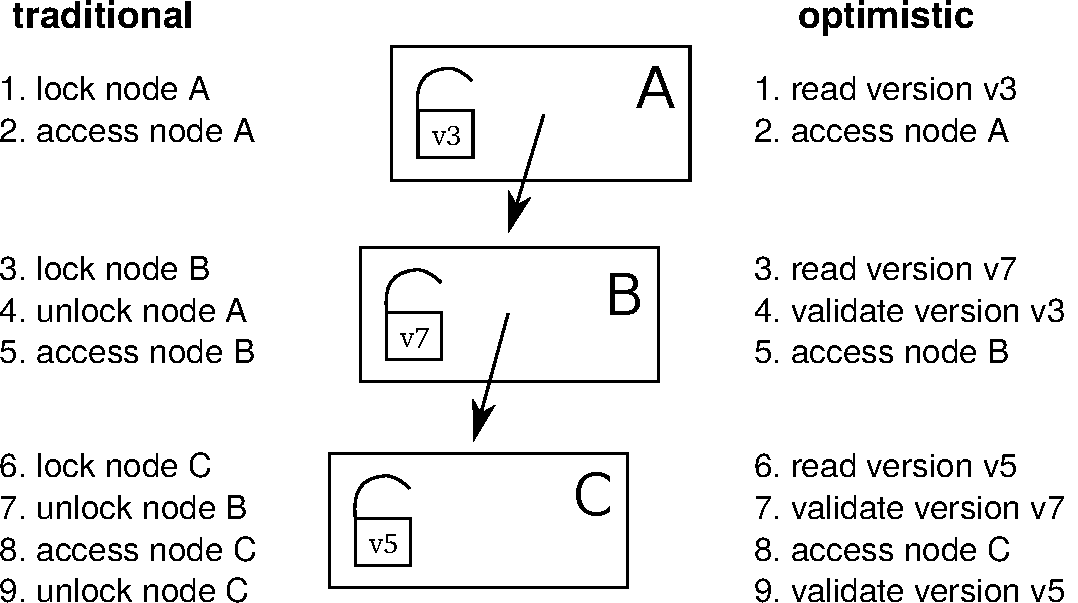
\includegraphics[width=0.65\linewidth]{olcall.pdf}
  \vspace{0.2cm}
  \caption{Comparison of a lookup operation in a 3-level tree using traditional lock coupling (left-hand side) vs.~optimistic lock coupling (right-hand side).}
  \label{fig:olc}
\end{figure}

The traditional and most common lock-based synchronization protocol for B-trees is lock coupling, which interleaves lock acquisitions while holding at most two locks at a time.
If, as we observed earlier, optimistic locks have similar semantics as traditional locks, it is natural to ask whether lock coupling can be combined with optimistic locks.
And indeed the answer is yes: One can almost mechanically translate traditional lock coupling code to optimistic lock coupling code.
This is illustrated in Figure~\ref{fig:olc}, which compares the traversal in a tree of height 3 using traditional and optimistic locks.
As the figure shows, the main difference is that locking is translated to reading the version and that unlocking becomes validation of the previously read version.
This simple change provides efficient lock-free tree traversal without the need to design a complex synchronization protocol.

It is important to emphasize the conceptual simplicity of OLC in comparison to data structures that use custom protocols like the Bw-tree~\cite{DBLP:conf/icde/LevandoskiLS13a}.
To implement lock-free access, the Bw-tree requires an indirection table, delta nodes, complex splitting and merging logic, retry logic, etc.
OLC, on the other hand, can directly be applied to B-trees mostly by adding the appropriate optimistic locking code and without modifying the node layout itself.
Therefore, OpenBw-Tree, an open source implementation of the Bw-tree, requires an order of magnitude more code than a B-tree based on OLC\footnote{Both implementations are available on GitHub: \url{https://github.com/wangziqi2016/index-microbench}}.
Given how difficult it is to develop, validate, and debug lock-free code, simplicity is obviously a major advantage.

\subsection{Correctness Aspects}

\begin{figure}
  % \centering
  %[basicstyle=\normalsize\ttfamily,showstringspaces=false,columns=fullflexible,breaklines=false,breakatwhitespace=true,numbers=none,numberstyle=\small,style=C,keepspaces=true]
\begin{lstlisting}[basicstyle=\ttfamily,language=C++,numbers=left,numberstyle=\small]
std::atomic<BTreeNode*> root;

// search for key in B+tree, returns payload in resultOut
bool lookup(Key key, Value& resultOut) {
   BTreeNode* node = root.load();
   uint64_t nodeVersion = node->readLockOrRestart();
   if (node != root.load()) // make sure the root is still the root
      restart();

   BTreeInner<Key>* parent = nullptr;
   uint64_t parentVersion = 0;

   while (node->isInner()) {
      auto inner = (BTreeInner*)node;

      // unlock parent and make current node the parent
      if (parent)
         parent->readUnlockOrRestart(parentVersion);
      parent = inner;
      parentVersion = nodeVersion;

      // search for next node
      node = inner->findChild(key);
      // validate 'inner' to ensure that 'node' pointer is valid
      inner->checkOrRestart(nodeVersion);
      // now it safe to dereference 'node' pointer (read its version)
      nodeVersion = node->readLockOrRestart();
   }

   // search in leaf and retrieve payload
   auto leaf = (BTreeLeaf*)node;
   bool success = leaf->findValue(key, resultOut);

   // unlock everything
   if (parent)
      parent->readUnlockOrRestart(parentVersion);
   node->readUnlockOrRestart(nodeVersion);

   return success;
}
\end{lstlisting}
  \vspace{0.2cm}
  \caption{B-tree lookup code using OLC. For simplicity, the restart logic is not shown.}
  \label{fig:lookup}
\end{figure}

So far, we have introduced the high-level ideas behind OLC and have stressed its similarity to traditional lock coupling.
Let us now discuss some cases where the close similarity between lock coupling and OLC breaks down.
To make this more concrete, we show the B-tree lookup code in Figure~\ref{fig:lookup}.
In the code, \texttt{readLockOrRestart} reads the lock version and \texttt{readUnlockOrRestart} validates that the read was correct.

One issue with OLC is that any pointer speculatively read from a node may point to invalid memory (if that node is modified concurrently).
Dereferencing such a pointer (e.g., to read its optimistic lock), may cause a segmentation fault or undefined behavior.
In the code shown in Figure~\ref{fig:lookup}, this problem is prevented by the extra check in line 25, which ensures that the read from the node containing the pointer was correct.
Without this additional validation, the code would in line 27 dereference the pointer speculatively read in line 23.
Note that the implementation of \texttt{checkOrRestart} is actually identical to \texttt{readUnlockOrRestart}.
We chose to give it a different name to highlight the fact that this extra check would not be necessary with read/write locks.

Another potential issue with optimistic locks is code that does not terminate.
Code that speculatively accesses a node, like an intra-node binary search, should be written in a way such that it always terminates---even in the presence of concurrent writes.
Otherwise, the validation code that detects the concurrent write will never run.
The binary search of a B-tree, for example, needs to be written in such a way that each comparison makes progress.
For some data structures that do not require loops in the traversal code (like ART) termination is trivially true.

\subsection{Implementation Details}

% implementation, efficiency
To implement an optimistic lock, one can combine the lock and the version counter into a single 64-bit\footnote{Even after subtracting one bit for the lock status, a back-of-the-envelope calculation can show that 63 bits are large enough to never overflow in practice.} word~\cite{artsync}.
A typical read operation will therefore merely consist of reading this version counter atomically.
In C++11 this can be implemented using the \texttt{std::atomic} type.

On x86, atomic reads are cheap because of x86's strong memory order guarantees.
No memory fences are required for sequentially-consistent loads, which are translated (by both GCC and clang) into standard \texttt{MOV} instructions.
Hence, the only effect of \texttt{std::atomic} for loads is preventing instruction re-ordering.
This makes version access and validation cheap.
Acquiring and releasing an optimistic lock in exclusive mode has comparable cost to a traditional lock:
A fairly expensive sequentially-consistent store is needed for acquiring a lock, while a standard \texttt{MOV} suffices for releasing it.
A simple sinlock-based implementation of optimistic locks can be found in the appendix of an earlier paper~\cite{artsync}.

OLC code must be able to handle restarts since validation or lock upgrade can fail due to concurrent writers.
Restarts can easily be implemented by wrapping the data structure operation in a loop (for simplicity not shown in Figure~\ref{fig:lookup}).
Such a loop also enables limiting the number of optimistic retry operations and falling back to pessimistic locking in cases of very heavy contention.
The ability to fall back to traditional locking is a major advantage of OLC in terms of robustness over lock-free approaches, which do not have this option.

In addition to the optimistic shared mode and the exclusive mode, optimistic locks also support a ``shared pessimistic'' mode, which physically acquires the lock in shared mode (allowing multiple concurrent readers but no writers).
This mode is useful for table (or range) scans that touch many tuples on a leaf page (which would otherwise easily abort).
Finally, let us mention that large range scans and table scans, should be broken up into several per-node traversals as is done in the LeanStore~\cite{leanstore} system.

Like all lock-free data structures, but unlike traditional locking and Hardware Transactional Memory~\cite{DBLP:conf/hpca/KarnagelDRLLSL14,DBLP:journals/pvldb/MakreshanskiLS15,htmtkde}, OLC requires care when deleting (and reusing) nodes.
The reason is that a deleting thread can never be sure that a node can be reclaimed because other threads might still be optimistically reading from that node.
Therefore, standard solutions like epoch-based reclamation~\cite{DBLP:conf/sosp/TuZKLM13}, hazard pointers~\cite{DBLP:journals/tpds/Michael04}, or optimized hazard pointers~\cite{DBLP:conf/spaa/BalmauGHZ16} need to be used.
These memory reclamation techniques are, however, largely orthogonal to the synchronization protocol itself.

%-lock-free is not a strong guarantee

\newpage
\section{Evaluation}\label{sec:evaluation}

Let us now experimentally evaluate the overhead and scalability of OLC.
For the experiments, we use an in-memory B+tree implemented in C++11 using templates, which is configured to use nodes of 4096 bytes, random 8 byte keys, and 8 byte payloads.
Based on this B-tree, we compare the following synchronization approaches:
\begin{itemize}
\item an OLC implementation\footnote{An almost identical OLC implementation is available on github: \url{https://github.com/wangziqi2016/index-microbench/tree/master/BTreeOLC}}
\item a variant based on traditional lock coupling and read/write locks
\item the unsynchronized B-tree, which obviously is only correct for read-only workloads but allows measuring the overhead of synchronization
\end{itemize}
Note that earlier work has compared the OLC implementation with a Bw-tree implementation~\cite{buzzword} and other state-of-the-art in-memory index structures.

We use a Haswell EP system with an Intel Xeon E5-2687W v3 CPU, which has 10 cores (20 ``Hyper-Threads'') and 25~MB of L3 cache.
The system is running Ubuntu 18.10 and we use GCC 8.2.0 to compile our code.
The CPU counters are obtained using the Linux perf API\footnote{We use the following convenience wrapper: \url{https://github.com/viktorleis/perfevent}}.

\begin{table}
  \caption{Performance and CPU counters for lookup and insert operations in a B-tree with 100M keys. We perform 100M operations and normalize the CPU counters by that number.}
  \label{tab:overhead}
  \centering
  \begin{tabular}{lrrrrrrr}\toprule
                    &         &        &        & instruc-  & L1     & L3     & branch \\
                    & threads & M op/s & cycles & tions & misses & misses & misses \\\midrule
lookup (no sync.)   & 1       & 1.72   & 2028   & 283     & 39.1   & 14.9   & 16.1   \\
lookup (OLC)        & 1       & 1.65   & 2107   & 370     & 43.9   & 15.1   & 16.7   \\
lookup (lock coup.) & 1       & 1.72   & 2078   & 365     & 42.3   & 16.9   & 15.7   \\\midrule
insert (no sync.)   & 1       & 1.51   & 2286   & 530     & 59.8   & 31.1   & 17.3   \\
insert (OLC)        & 1       & 1.50   & 2303   & 629     & 61.2   & 31.1   & 16.5   \\
insert (lock coup.) & 1       & 1.41   & 2473   & 644     & 61.0   & 31.0   & 17.2   \\\midrule
lookup (no sync.)   & 10      & 15.48  & 2058   & 283     & 38.6   & 15.5   & 16.0   \\
lookup (OLC)        & 10      & 14.60  & 2187   & 370     & 43.8   & 15.8   & 16.8   \\
lookup (lock coup.) & 10      & 5.71   & 5591   & 379     & 54.2   & 17.0   & 14.8   \\\midrule
insert (no sync.)   & 10      & -      & -      & -       & -      & -      & -      \\
insert (OLC)        & 10      & 10.46  & 2940   & 656     & 62.0   & 32.5   & 16.8   \\
insert (lock coup.) & 10      & 7.55   & 4161   & 667     & 75.0   & 28.6   & 16.2   \\
    \bottomrule
\end{tabular}
\end{table}

Table~\ref{tab:overhead} compares the performance and CPU counters for lookup and insert operations in a B-tree with 100M keys.
With {\em single-threaded} execution, we observe that all three approaches have very similar performance.
Adding traditional or optimistic locks to unsynchronized B-tree code results in up to 30\% of additional instructions without affecting single-threaded performance much.

\begin{figure}
  \centering
  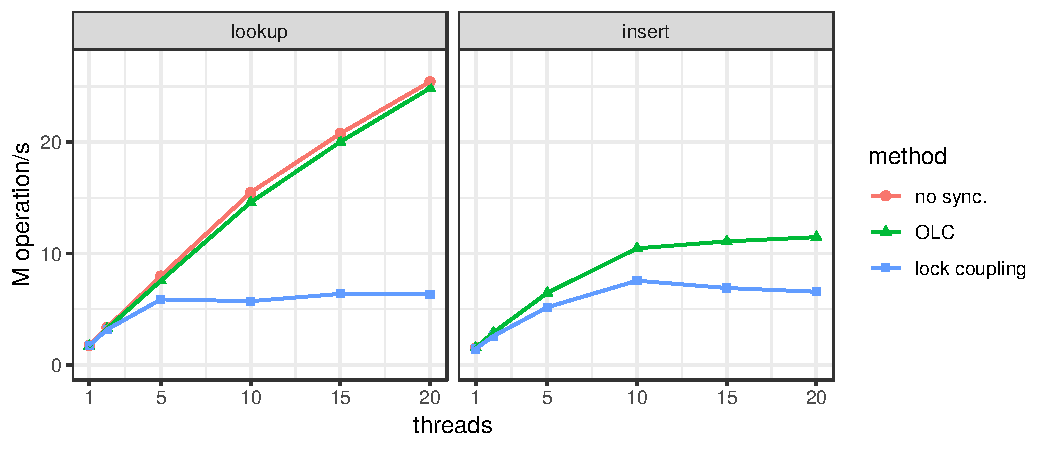
\includegraphics[width=\linewidth]{scale.pdf}
  \vspace{0.2cm}
  \caption{Scalability on 10-core system for B-tree operations (100M values).}
  \label{fig:scale}
\end{figure}

As Figure~\ref{fig:scale} shows, the results change dramatically once we use multiple threads.
For lookup, the scalability of OLC is near-linear up to 20 threads, even though the system has only 10 ``real cores''.
The OLC scalability for insert is also respectable (though not quite as linear because multi-threaded insertion approaches the memory bandwidth of our processor).
The figure also shows that the results of traditional lock coupling with read/write locks are significantly worse than OLC.
With 20 threads, lookup with OLC is 3.9$\times$ faster than traditional lock coupling.

\section{Summary}\label{sec:conc}

Optimistic Lock Coupling (OLC) is an effective synchronization method that combines the simplicity of traditional lock coupling with the superior scalability of lock-free approaches.
OLC is widely applicable and has already been successfully used to synchronize several data structures, including B-trees, binary search trees, and different trie variants.
These features make it highly attractive for modern database systems as well as performance-critical systems software in general.

\begin{thebibliography}{10}

\bibitem{DBLP:conf/spaa/BalmauGHZ16}
O.~Balmau, R.~Guerraoui, M.~Herlihy, and I.~Zablotchi.
\newblock Fast and robust memory reclamation for concurrent data structures.
\newblock In {\em SPAA}, 2016.

\bibitem{DBLP:journals/acta/BayerS77}
R.~Bayer and M.~Schkolnick.
\newblock Concurrency of operations on {B}-trees.
\newblock {\em Acta Informatica}, 9, 1977.

\bibitem{hot}
R.~Binna, E.~Zangerle, M.~Pichl, G.~Specht, and V.~Leis.
\newblock {HOT}: A height optimized trie index for main-memory database
  systems.
\newblock In {\em SIGMOD}, 2018.

\bibitem{DBLP:conf/ppopp/BronsonCCO10}
N.~G. Bronson, J.~Casper, H.~Chafi, and K.~Olukotun.
\newblock A practical concurrent binary search tree.
\newblock In {\em PPOPP}, 2010.

\bibitem{DBLP:conf/vldb/ChaHKK01}
S.~K. Cha, S.~Hwang, K.~Kim, and K.~Kwon.
\newblock Cache-conscious concurrency control of main-memory indexes on
  shared-memory multiprocessor systems.
\newblock In {\em VLDB}, 2001.

\bibitem{intel}
I.~Cutress.
\newblock {Intel} goes for 48-cores: {Cascade-AP} with multi-chip package
  coming soon.
\newblock
  \url{https://www.anandtech.com/show/13535/intel-goes-for-48cores-cascade-ap},
  2018 (accessed January, 2019).

\bibitem{DBLP:conf/cidr/FaleiroA17}
J.~M. Faleiro and D.~J. Abadi.
\newblock Latch-free synchronization in database systems: Silver bullet or
  fool's gold?
\newblock In {\em CIDR}, 2017.

\bibitem{DBLP:journals/ftdb/Graefe11}
G.~Graefe.
\newblock Modern {B}-tree techniques.
\newblock {\em Foundations and Trends in Databases}, 3(4), 2011.

\bibitem{DBLP:conf/hpca/KarnagelDRLLSL14}
T.~Karnagel, R.~Dementiev, R.~Rajwar, K.~Lai, T.~Legler, B.~Schlegel, and
  W.~Lehner.
\newblock Improving in-memory database index performance with
  {Intel}\({}^{\mbox{{\textregistered}}}\) transactional synchronization
  extensions.
\newblock In {\em HPCA}, 2014.

\bibitem{DBLP:journals/tods/LehmanY81}
P.~L. Lehman and S.~B. Yao.
\newblock Efficient locking for concurrent operations on {B}-trees.
\newblock {\em {ACM} Trans. Database Syst.}, 6(4), 1981.

\bibitem{leanstore}
V.~Leis, M.~Haubenschild, A.~Kemper, and T.~Neumann.
\newblock Leanstore: In-memory data management beyond main memory.
\newblock In {\em ICDE}, 2018.

\bibitem{art}
V.~Leis, A.~Kemper, and T.~Neumann.
\newblock The adaptive radix tree: {ARTful} indexing for main-memory databases.
\newblock In {\em ICDE}, 2013.

\bibitem{htmtkde}
V.~Leis, A.~Kemper, and T.~Neumann.
\newblock Scaling {HTM}-supported database transactions to many cores.
\newblock {\em {IEEE} Trans. Knowl. Data Eng.}, 28(2), 2016.

\bibitem{artsync}
V.~Leis, F.~Scheibner, A.~Kemper, and T.~Neumann.
\newblock The {ART} of practical synchronization.
\newblock In {\em DaMoN}, 2016.

\bibitem{DBLP:conf/icde/LevandoskiLS13a}
J.~J. Levandoski, D.~B. Lomet, and S.~Sengupta.
\newblock The {Bw}-tree: A {B}-tree for new hardware platforms.
\newblock In {\em ICDE}, 2013.

\bibitem{DBLP:journals/pvldb/MakreshanskiLS15}
D.~Makreshanski, J.~J. Levandoski, and R.~Stutsman.
\newblock To lock, swap, or elide: On the interplay of hardware transactional
  memory and lock-free indexing.
\newblock {\em {PVLDB}}, 8(11), 2015.

\bibitem{DBLP:dblp_conf/eurosys/MaoKM12}
Y.~Mao, E.~Kohler, and R.~T. Morris.
\newblock Cache craftiness for fast multicore key-value storage.
\newblock In {\em EuroSys}, 2012.

\bibitem{DBLP:journals/tpds/Michael04}
M.~M. Michael.
\newblock Hazard pointers: Safe memory reclamation for lock-free objects.
\newblock {\em {IEEE} Trans. Parallel Distrib. Syst.}, 15(6), 2004.

\bibitem{DBLP:journals/jacm/ShalevS06}
O.~Shalev and N.~Shavit.
\newblock Split-ordered lists: Lock-free extensible hash tables.
\newblock {\em J. {ACM}}, 53(3), 2006.

\bibitem{amd}
A.~Shilov.
\newblock {AMD} previews {EPYC} ‘{Rome}’ processor: Up to 64 {Zen} 2 cores.
\newblock
  \url{https://www.anandtech.com/show/13561/amd-previews-epyc-rome-processor-up-to-64-zen-2-cores},
  2018 (accessed January, 2019).

\bibitem{DBLP:conf/sosp/TuZKLM13}
S.~Tu, W.~Zheng, E.~Kohler, B.~Liskov, and S.~Madden.
\newblock Speedy transactions in multicore in-memory databases.
\newblock In {\em SOSP}, 2013.

\bibitem{buzzword}
Z.~Wang, A.~Pavlo, H.~Lim, V.~Leis, H.~Zhang, M.~Kaminsky, and D.~Andersen.
\newblock Building a {Bw}-tree takes more than just buzz words.
\newblock In {\em SIGMOD}, 2018.

\end{thebibliography}


%\bibliographystyle{abbrv}
%\bibliography{main}

\end{document}

\end{article}


\begin{article}
{Data Management for Causal Algorithmic Fairness}
{Babak Salimi, Bill Howe, Dan Suciu}
\graphicspath{{submissions/Salimi/salimi/}}
\pdfminorversion=5
\documentclass[11pt]{article}
\usepackage{deauthor,times,graphicx,caption,microtype}
\usepackage{hyperref}
\usepackage{listings}
\usepackage{booktabs}

\begin{document}

\title{Optimistic Lock Coupling: A Scalable and Efficient General-Purpose Synchronization Method}

\author{Viktor Leis, Michael Haubenschild\raisebox{0.9ex}{$\ast$}, Thomas Neumann\\ Technische Universit{\"a}t M{\"u}nchen \hspace{0.7cm} Tableau Software\raisebox{0.9ex}{$\ast$} \\ {\{leis,neumann\}{@}in.tum.de} \hspace{0.7cm} {mhaubenschild{@}tableau.com\raisebox{0.9ex}{$\ast$}}}

\maketitle

\begin{abstract}
As the number of cores on commodity processors continues to increase, scalability becomes more and more crucial for overall performance.
Scalable and efficient concurrent data structures are particularly important, as these are often the building blocks of parallel algorithms.
Unfortunately, traditional synchronization techniques based on fine-grained locking have been shown to be unscalable on modern multi-core CPUs.
Lock-free data structures, on the other hand, are extremely difficult to design and often incur significant overhead.

In this work, we make the case for Optimistic Lock Coupling as a practical alternative to both traditional locking and the lock-free approach.
We show that Optimistic Lock Coupling is highly scalable and almost as simple to implement as traditional lock coupling.
Another important advantage is that it is easily applicable to most tree-like data structures.
We therefore argue that Optimistic Lock Coupling, rather than a complex and error-prone custom synchronization protocol, should be the default choice for performance-critical data structures.
\end{abstract}

\section{Introduction}

% more and more cores
Today, Intel's commodity server processors have up to 28 cores and its upcoming microarchitecture will have up to 48 cores per socket~\cite{intel}.
Similarly, AMD currently stands at 32 cores and this number is expected to double in the next generation~\cite{amd}.
Since both platforms support simultaneous multithreading (also known as hyperthreading), affordable commodity servers (with up to two sockets) will soon routinely have between 100 and 200 hardware threads.

% data structure scalability is important
With such a high degree of hardware parallelism, efficient data processing crucially depends on how well concurrent data structures scale.
Internally, database systems use a plethora of data structures like table heaps, internal work queues, and, most importantly, index structures.
Any of these can easily become a scalability (and therefore overall performance) bottleneck on many-core CPUs.

% traditional synchronization: fine-grained locks, slow, cache invalidation
Traditionally, database systems synchronize internal data structures using fine-grained reader/writer locks\footnote{In this work, we focus on data structure synchronization rather than high-level transaction semantics and therefore use the term {\em lock} for what would typically be called {\em latch} in the database literature. We thus follow common computer science (rather than database) terminology.}.
Unfortunately, while fine-grained locking makes lock contention unlikely, it still results in bad scalability because lock acquisition and release require writing to shared memory.
Due to the way cache coherency is implemented on modern multi-core CPUs, these writes cause additional cache misses\footnote{The cache coherency protocol ensures that all copies of a cache line on other cores are invalidated before the write can proceed.} and the cache line containing the lock's internal data becomes a point of physical contention.
As a result, any frequently-accessed lock (e.g., the lock of the root node of a B-tree) severely limits scalability.

% lock-free bw-tree: no more latches, but indirections, extremely complex
Lock-free data structures like the Bw-tree~\cite{DBLP:conf/icde/LevandoskiLS13a} (a lock-free B-tree variant) or the Split-Ordered List~\cite{DBLP:journals/jacm/ShalevS06} (a lock-free hash table) do not acquire any locks and therefore generally scale much better than locking-based approaches (in particular for read-mostly workloads).
However, lock-free synchronization has other downsides:
First, it is very difficult and results in extremely complex and error-prone code (when compared to locking).
Second, because the functionality of atomic primitives provided by the hardware (e.g., atomically compare-and-swap 8 bytes) is limited, complex operations require additional indirections within the data structure.
For example, the Bw-tree requires an indirection table and the Split-Ordered List requires ``dummy nodes'', resulting in overhead due to additional cache misses.

% OLC for the win
In this paper we make the case for {\em Optimistic Lock Coupling (OLC)}, a synchronization method that combines some of the best properties of lock-based and lock-free synchronization.
OLC utilizes a special lock type that can be used in two modes:
The first mode is similar to a traditional mutex and excludes other threads by physically acquiring the underlying lock.
In the second mode, reads can proceed optimistically by validating a version counter that is embedded in the lock (similar to optimistic concurrency control).
The first mode is typically used by writers and the second mode by readers.
Besides this special lock type, OLC is based on the observation that optimistic lock validations can be interleaved/coupled---similar to the pair-wise interleaved lock acquisition of traditional lock coupling.
Hence, the name Optimistic Lock Coupling.

OLC has a number of desirable features:
\begin{itemize}
\item By reducing the number of writes to shared memory locations and thereby avoiding cache invalidations, it {\bf scales well} for most workloads.
\item In comparison to unsynchronized code, it requires few additional CPU instructions making it {\bf efficient}.
\item OLC is {\bf widely applicable} to different data structures. It has already been successfully used for synchronizing binary search trees~\cite{DBLP:conf/ppopp/BronsonCCO10}, tries~\cite{artsync}, trie/B-tree hybrids~\cite{DBLP:dblp_conf/eurosys/MaoKM12}, and B-trees~\cite{buzzword}.
\item In comparison to the lock-free paradigm, it is also {\bf easy to use} and requires few modifications to existing, single-threaded data structures.
\end{itemize}
Despite these positive features and its simplicity, OLC is not yet widely known.
The goal of this paper is therefore to popularize this simple idea and to make a case for it.
We argue that OLC deserves to be widely known.
It is a good default synchronization paradigm---more complex, data structure-specific protocols are seldom beneficial.

The rest of the paper is organized as follows.
Section~\ref{sec:related} discusses related work, tracing the history of OLC and its underlying ideas in the literature.
The core of the paper is Section~\ref{sec:olc}, which describes the ideas behind OLC and how it can be used to synchronize complex data structures.
In Section~\ref{sec:evaluation} we experimentally show that OLC has low overhead and scales well when used to synchronize an in-memory B-tree.
We summarize the paper in Section~\ref{sec:conc}.

\newpage
\section{Related Work}\label{sec:related}

Lock coupling has been proposed as a method for allowing concurrent operations on B-trees in 1977~\cite{DBLP:journals/acta/BayerS77}.
This traditional and still widely-used method, described in detail in Graefe's B-tree survey~\cite{DBLP:journals/ftdb/Graefe11}, is also called ``latch coupling'', ``hand-over-hand locking'', and ``crabbing''.
Because at most two locks are held at-a-time during tree traversal, this technique seemingly allows for a high degree of parallelism---in particular if read/write locks are used to enable inner nodes to be locked in shared mode.
However, as we show in Section~\ref{sec:evaluation}, on modern hardware lock acquisition (even in shared mode) results in suboptimal scalability.

An early alternative from 1981 is a B-tree variant called B-link tree~\cite{DBLP:journals/tods/LehmanY81}, which only holds a single lock at a time.
It is based on the observation that between the release of the parent lock and the acquisition of the child lock, the only ``dangerous'' thing that could have happened is the split of a child node (assuming one does not implement merge operations).
Thus, when a split happens, the key being searched might end up on a neighboring node to the right of the current child node.
A B-link tree traversal therefore detects this condition and, if needed, transparently proceeds to the neighboring node.
Releasing the parent lock early is highly beneficial when the child node needs to be fetched from disk.
For in-memory workloads, however, the B-link tree has the same scalability issues as lock coupling (it acquires just as many locks).

The next major advance, Optimistic Latch-Free Index Traversal (OLFIT)~\cite{DBLP:conf/vldb/ChaHKK01}, was proposed in 2001.
OLFIT introduced the idea of a combined lock/update counter, which we call {\em optimistic lock}. % , for lack of a better name,
Based on these per-node optimistic locks and the synchronization protocol of the B-link tree, OLFIT finally achieves good scalability on parallel processors.
The OLFIT protocol is fairly complex, as it requires both the non-trivial B-link protocol and optimistic locks.
Furthermore, like the B-link tree protocol, it does not support merging nodes, and is specific to B-trees (cannot easily be applied to other data structures).

In the following two decades, the growth of main-memory capacity led to much research into other data structures besides the venerable B-tree.
Particularly relevant for our discussion is Bronson et al.'s~\cite{DBLP:conf/ppopp/BronsonCCO10} concurrent binary search tree, which is based on optimistic version validation and has a sophisticated, data structure-specific synchronization protocol.
To the best of our knowledge, this 2010 paper is the first that, as part of its protocol, interleaves version validation across nodes---rather than validating each node separately like OLFIT.
In that paper, this idea is called ``hand-over-hand, optimistic validation'', while we prefer the term Optimistic Lock Coupling to highlight the close resemblance to traditional lock coupling.
Similarly, Mao et al.'s~\cite{DBLP:dblp_conf/eurosys/MaoKM12} Masstree (a concurrent hybrid trie/B-tree) is also based on the same ideas, but again uses them as part of a more complex protocol.

The Adaptive Radix Tree (ART)~\cite{art} is another recent in-memory data structure, which we proposed in 2013.
In contrast to the two data structures just mentioned, it was originally designed with single-threaded performance in mind without supporting concurrency.
To add support for concurrency, we initially started designing a custom protocol called Read-Optimized Write Exclusion (ROWEX)~\cite{artsync}, which turned out to be non-trivial and requires modifications of the underlying data structure\footnote{Note that ROWEX is already easier to apply to existing data structures than the lock-free approach. The difficulty depends on the data structure. Applying ROWEX is hard for B-trees with sorted keys and fairly easy for copy-on-write data structures like the Height Optimized Trie~\cite{hot}---with ART being somewhere in the middle.}.
However, fairly late in the project, we also realized, that OLC {\em alone} (rather than as part of a more complex protocol) is sufficient to synchronize ART.
No other changes to the data structure were necessary.
Both approaches were published and experimentally evaluated in a followup paper~\cite{artsync}, which shows that, despite its simplicity, OLC is efficient, scalable, and generally outperforms ROWEX.

Similar results were recently published regarding B-trees~\cite{buzzword}.
In this experimental study a simple OLC-based synchronization outperformed the Bw-tree~\cite{DBLP:conf/icde/LevandoskiLS13a}, a complex lock-free synchronization approach.
Another recent paper shows that for write-intensive workloads, locking often performs better than lock-free synchronization~\cite{DBLP:conf/cidr/FaleiroA17}.
These experiences indicate that OLC is a general-purpose synchronization paradigm and motivate the current paper.

%foster b-tree\cite{DBLP:journals/tods/GraefeKK12}
%Shasha theory~\cite{DBLP:journals/tods/ShashaG88}

\section{Optimistic Lock Coupling}\label{sec:olc}

% locks suck
The standard technique for inter-thread synchronization is mutual exclusion using fine-grained locks.
In a B-tree, for example, every node usually has its own associated lock, which is acquired before accessing that node.
The problem of locking on modern multi- and many-core processors is that lock acquisition and release require writing to the shared memory location that implements the lock.
This write causes exclusive ownership of the underlying cache line and invalidates copies of it on all other processor cores.
For hierarchical, tree-like data structures, the lock of the root node becomes a point of physical contention---even in read-only workloads and even when read/write locks are used.
Depending on the specific data structure, number of cores, cache coherency protocol implementation, cache topology, whether Non-Uniform Memory Access (NUMA) is used, locking can even result in multi-threaded performance that is worse than single-threaded execution.

% in b-trees this happens very much
The inherent pessimism of locking is particularly unfortunate for B-trees:
Despite the fact that logical modifications of the root node are very infrequent, every B-tree operation must lock the root node during tree traversal\footnote{To a lesser extent this obviously applies to all inner nodes, not just the root.}.
Even the vast majority of update operations (with the exception of splits and merges), only modify a single leaf node.
These observations indicate that a more optimistic approach, which does not require locking inner nodes, would be very beneficial for B-trees.

\subsection{Optimistic Locks}

% optimism to the rescue
As the name indicates, optimistic locks try to solve the scalability issues of traditional locks using an optimistic approach.
Instead of always physically acquiring locks, even for nodes that are unlikely to be modified simultaneously, after-the-fact validation is used to detect conflicts.
This is done by augmenting each lock with a version/update counter that is incremented on every modification.
Using this version counter, readers can optimistically proceed before validating that the version did not change to ensure that the read was safe.
If validation fails, the operation is restarted.

% details on opt locks
Using optimistic locks, a read-only node access (i.e., the majority of all operations in a B-tree) does not acquire the lock and does not increment the version counter.
Instead, it performs the following steps:
\begin{enumerate}
\item read lock version (restart if lock is not free)
\item access node
\item read the version again and validate that it has not changed in the meantime
\end{enumerate}
If the last step (the validation) fails, the operation has to be restarted.
Write operations, on the other hand, are more similar to traditional locking:
\begin{enumerate}
\item acquire lock (wait if necessary)
\item access/write to node
\item increment version and unlock node
\end{enumerate}
Writes can therefore protect a node from other writes.

% similar to locks
As we observed in an earlier paper~\cite{artsync}, because of similar semantics, optimistic locks can be hidden behind an API very similar to traditional read/write locks.
Both approaches have an exclusive lock mode, and acquiring a traditional lock in shared mode is analogous to optimistic version validation.
Furthermore, like with some implementations of traditional read/write locks, optimistic locks allow upgrading a shared lock to an exclusive lock.
Lock upgrades are, for example, used to avoid most B-tree update operations from having to lock inner nodes.
In our experience, the close resemblance of optimistic and traditional locks simplifies the reasoning about optimistic locks;
one can apply similar thinking as in traditional lock-based protocols.

\subsection{Lock Coupling with Optimistic Locks}

\begin{figure}
  \centering
  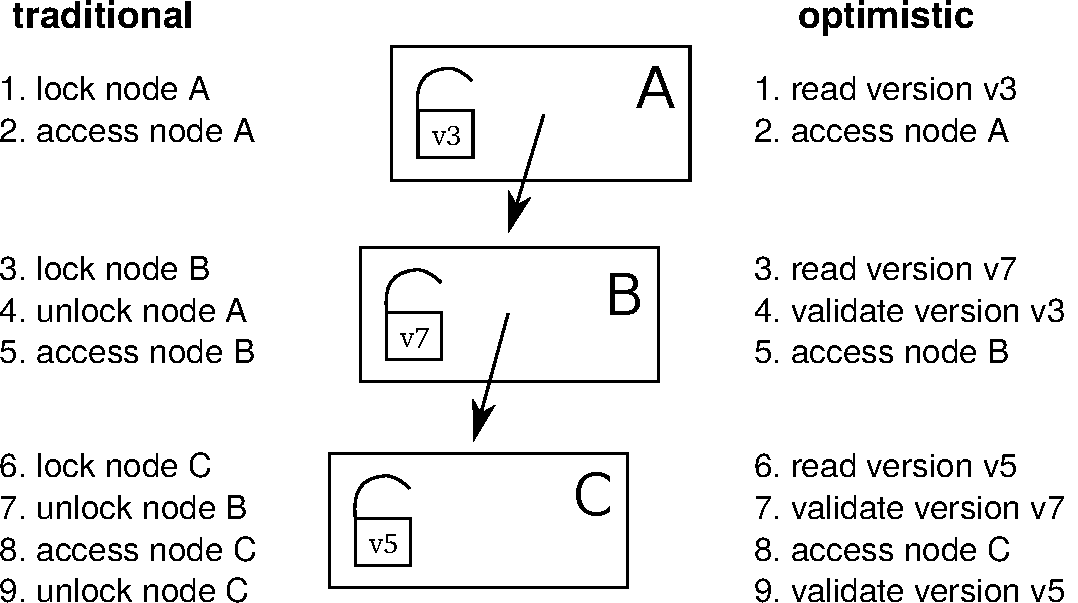
\includegraphics[width=0.65\linewidth]{olcall.pdf}
  \vspace{0.2cm}
  \caption{Comparison of a lookup operation in a 3-level tree using traditional lock coupling (left-hand side) vs.~optimistic lock coupling (right-hand side).}
  \label{fig:olc}
\end{figure}

The traditional and most common lock-based synchronization protocol for B-trees is lock coupling, which interleaves lock acquisitions while holding at most two locks at a time.
If, as we observed earlier, optimistic locks have similar semantics as traditional locks, it is natural to ask whether lock coupling can be combined with optimistic locks.
And indeed the answer is yes: One can almost mechanically translate traditional lock coupling code to optimistic lock coupling code.
This is illustrated in Figure~\ref{fig:olc}, which compares the traversal in a tree of height 3 using traditional and optimistic locks.
As the figure shows, the main difference is that locking is translated to reading the version and that unlocking becomes validation of the previously read version.
This simple change provides efficient lock-free tree traversal without the need to design a complex synchronization protocol.

It is important to emphasize the conceptual simplicity of OLC in comparison to data structures that use custom protocols like the Bw-tree~\cite{DBLP:conf/icde/LevandoskiLS13a}.
To implement lock-free access, the Bw-tree requires an indirection table, delta nodes, complex splitting and merging logic, retry logic, etc.
OLC, on the other hand, can directly be applied to B-trees mostly by adding the appropriate optimistic locking code and without modifying the node layout itself.
Therefore, OpenBw-Tree, an open source implementation of the Bw-tree, requires an order of magnitude more code than a B-tree based on OLC\footnote{Both implementations are available on GitHub: \url{https://github.com/wangziqi2016/index-microbench}}.
Given how difficult it is to develop, validate, and debug lock-free code, simplicity is obviously a major advantage.

\subsection{Correctness Aspects}

\begin{figure}
  % \centering
  %[basicstyle=\normalsize\ttfamily,showstringspaces=false,columns=fullflexible,breaklines=false,breakatwhitespace=true,numbers=none,numberstyle=\small,style=C,keepspaces=true]
\begin{lstlisting}[basicstyle=\ttfamily,language=C++,numbers=left,numberstyle=\small]
std::atomic<BTreeNode*> root;

// search for key in B+tree, returns payload in resultOut
bool lookup(Key key, Value& resultOut) {
   BTreeNode* node = root.load();
   uint64_t nodeVersion = node->readLockOrRestart();
   if (node != root.load()) // make sure the root is still the root
      restart();

   BTreeInner<Key>* parent = nullptr;
   uint64_t parentVersion = 0;

   while (node->isInner()) {
      auto inner = (BTreeInner*)node;

      // unlock parent and make current node the parent
      if (parent)
         parent->readUnlockOrRestart(parentVersion);
      parent = inner;
      parentVersion = nodeVersion;

      // search for next node
      node = inner->findChild(key);
      // validate 'inner' to ensure that 'node' pointer is valid
      inner->checkOrRestart(nodeVersion);
      // now it safe to dereference 'node' pointer (read its version)
      nodeVersion = node->readLockOrRestart();
   }

   // search in leaf and retrieve payload
   auto leaf = (BTreeLeaf*)node;
   bool success = leaf->findValue(key, resultOut);

   // unlock everything
   if (parent)
      parent->readUnlockOrRestart(parentVersion);
   node->readUnlockOrRestart(nodeVersion);

   return success;
}
\end{lstlisting}
  \vspace{0.2cm}
  \caption{B-tree lookup code using OLC. For simplicity, the restart logic is not shown.}
  \label{fig:lookup}
\end{figure}

So far, we have introduced the high-level ideas behind OLC and have stressed its similarity to traditional lock coupling.
Let us now discuss some cases where the close similarity between lock coupling and OLC breaks down.
To make this more concrete, we show the B-tree lookup code in Figure~\ref{fig:lookup}.
In the code, \texttt{readLockOrRestart} reads the lock version and \texttt{readUnlockOrRestart} validates that the read was correct.

One issue with OLC is that any pointer speculatively read from a node may point to invalid memory (if that node is modified concurrently).
Dereferencing such a pointer (e.g., to read its optimistic lock), may cause a segmentation fault or undefined behavior.
In the code shown in Figure~\ref{fig:lookup}, this problem is prevented by the extra check in line 25, which ensures that the read from the node containing the pointer was correct.
Without this additional validation, the code would in line 27 dereference the pointer speculatively read in line 23.
Note that the implementation of \texttt{checkOrRestart} is actually identical to \texttt{readUnlockOrRestart}.
We chose to give it a different name to highlight the fact that this extra check would not be necessary with read/write locks.

Another potential issue with optimistic locks is code that does not terminate.
Code that speculatively accesses a node, like an intra-node binary search, should be written in a way such that it always terminates---even in the presence of concurrent writes.
Otherwise, the validation code that detects the concurrent write will never run.
The binary search of a B-tree, for example, needs to be written in such a way that each comparison makes progress.
For some data structures that do not require loops in the traversal code (like ART) termination is trivially true.

\subsection{Implementation Details}

% implementation, efficiency
To implement an optimistic lock, one can combine the lock and the version counter into a single 64-bit\footnote{Even after subtracting one bit for the lock status, a back-of-the-envelope calculation can show that 63 bits are large enough to never overflow in practice.} word~\cite{artsync}.
A typical read operation will therefore merely consist of reading this version counter atomically.
In C++11 this can be implemented using the \texttt{std::atomic} type.

On x86, atomic reads are cheap because of x86's strong memory order guarantees.
No memory fences are required for sequentially-consistent loads, which are translated (by both GCC and clang) into standard \texttt{MOV} instructions.
Hence, the only effect of \texttt{std::atomic} for loads is preventing instruction re-ordering.
This makes version access and validation cheap.
Acquiring and releasing an optimistic lock in exclusive mode has comparable cost to a traditional lock:
A fairly expensive sequentially-consistent store is needed for acquiring a lock, while a standard \texttt{MOV} suffices for releasing it.
A simple sinlock-based implementation of optimistic locks can be found in the appendix of an earlier paper~\cite{artsync}.

OLC code must be able to handle restarts since validation or lock upgrade can fail due to concurrent writers.
Restarts can easily be implemented by wrapping the data structure operation in a loop (for simplicity not shown in Figure~\ref{fig:lookup}).
Such a loop also enables limiting the number of optimistic retry operations and falling back to pessimistic locking in cases of very heavy contention.
The ability to fall back to traditional locking is a major advantage of OLC in terms of robustness over lock-free approaches, which do not have this option.

In addition to the optimistic shared mode and the exclusive mode, optimistic locks also support a ``shared pessimistic'' mode, which physically acquires the lock in shared mode (allowing multiple concurrent readers but no writers).
This mode is useful for table (or range) scans that touch many tuples on a leaf page (which would otherwise easily abort).
Finally, let us mention that large range scans and table scans, should be broken up into several per-node traversals as is done in the LeanStore~\cite{leanstore} system.

Like all lock-free data structures, but unlike traditional locking and Hardware Transactional Memory~\cite{DBLP:conf/hpca/KarnagelDRLLSL14,DBLP:journals/pvldb/MakreshanskiLS15,htmtkde}, OLC requires care when deleting (and reusing) nodes.
The reason is that a deleting thread can never be sure that a node can be reclaimed because other threads might still be optimistically reading from that node.
Therefore, standard solutions like epoch-based reclamation~\cite{DBLP:conf/sosp/TuZKLM13}, hazard pointers~\cite{DBLP:journals/tpds/Michael04}, or optimized hazard pointers~\cite{DBLP:conf/spaa/BalmauGHZ16} need to be used.
These memory reclamation techniques are, however, largely orthogonal to the synchronization protocol itself.

%-lock-free is not a strong guarantee

\newpage
\section{Evaluation}\label{sec:evaluation}

Let us now experimentally evaluate the overhead and scalability of OLC.
For the experiments, we use an in-memory B+tree implemented in C++11 using templates, which is configured to use nodes of 4096 bytes, random 8 byte keys, and 8 byte payloads.
Based on this B-tree, we compare the following synchronization approaches:
\begin{itemize}
\item an OLC implementation\footnote{An almost identical OLC implementation is available on github: \url{https://github.com/wangziqi2016/index-microbench/tree/master/BTreeOLC}}
\item a variant based on traditional lock coupling and read/write locks
\item the unsynchronized B-tree, which obviously is only correct for read-only workloads but allows measuring the overhead of synchronization
\end{itemize}
Note that earlier work has compared the OLC implementation with a Bw-tree implementation~\cite{buzzword} and other state-of-the-art in-memory index structures.

We use a Haswell EP system with an Intel Xeon E5-2687W v3 CPU, which has 10 cores (20 ``Hyper-Threads'') and 25~MB of L3 cache.
The system is running Ubuntu 18.10 and we use GCC 8.2.0 to compile our code.
The CPU counters are obtained using the Linux perf API\footnote{We use the following convenience wrapper: \url{https://github.com/viktorleis/perfevent}}.

\begin{table}
  \caption{Performance and CPU counters for lookup and insert operations in a B-tree with 100M keys. We perform 100M operations and normalize the CPU counters by that number.}
  \label{tab:overhead}
  \centering
  \begin{tabular}{lrrrrrrr}\toprule
                    &         &        &        & instruc-  & L1     & L3     & branch \\
                    & threads & M op/s & cycles & tions & misses & misses & misses \\\midrule
lookup (no sync.)   & 1       & 1.72   & 2028   & 283     & 39.1   & 14.9   & 16.1   \\
lookup (OLC)        & 1       & 1.65   & 2107   & 370     & 43.9   & 15.1   & 16.7   \\
lookup (lock coup.) & 1       & 1.72   & 2078   & 365     & 42.3   & 16.9   & 15.7   \\\midrule
insert (no sync.)   & 1       & 1.51   & 2286   & 530     & 59.8   & 31.1   & 17.3   \\
insert (OLC)        & 1       & 1.50   & 2303   & 629     & 61.2   & 31.1   & 16.5   \\
insert (lock coup.) & 1       & 1.41   & 2473   & 644     & 61.0   & 31.0   & 17.2   \\\midrule
lookup (no sync.)   & 10      & 15.48  & 2058   & 283     & 38.6   & 15.5   & 16.0   \\
lookup (OLC)        & 10      & 14.60  & 2187   & 370     & 43.8   & 15.8   & 16.8   \\
lookup (lock coup.) & 10      & 5.71   & 5591   & 379     & 54.2   & 17.0   & 14.8   \\\midrule
insert (no sync.)   & 10      & -      & -      & -       & -      & -      & -      \\
insert (OLC)        & 10      & 10.46  & 2940   & 656     & 62.0   & 32.5   & 16.8   \\
insert (lock coup.) & 10      & 7.55   & 4161   & 667     & 75.0   & 28.6   & 16.2   \\
    \bottomrule
\end{tabular}
\end{table}

Table~\ref{tab:overhead} compares the performance and CPU counters for lookup and insert operations in a B-tree with 100M keys.
With {\em single-threaded} execution, we observe that all three approaches have very similar performance.
Adding traditional or optimistic locks to unsynchronized B-tree code results in up to 30\% of additional instructions without affecting single-threaded performance much.

\begin{figure}
  \centering
  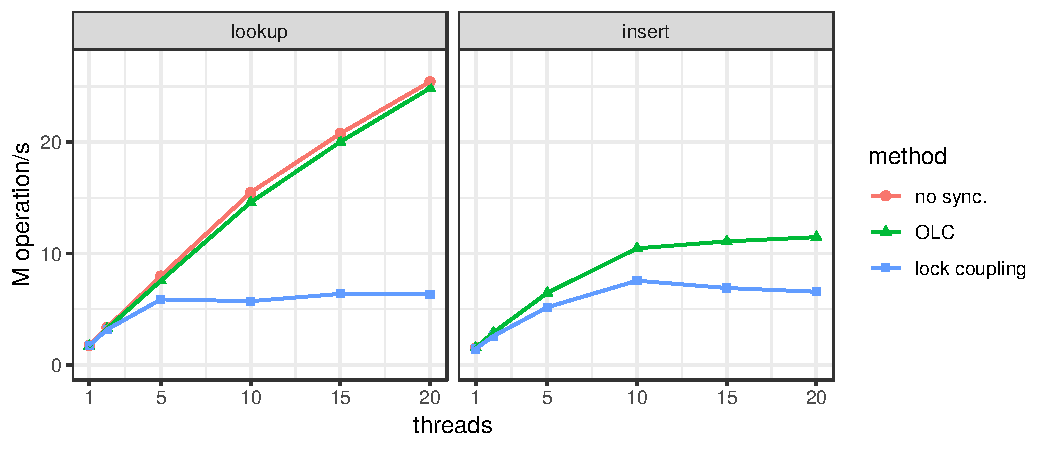
\includegraphics[width=\linewidth]{scale.pdf}
  \vspace{0.2cm}
  \caption{Scalability on 10-core system for B-tree operations (100M values).}
  \label{fig:scale}
\end{figure}

As Figure~\ref{fig:scale} shows, the results change dramatically once we use multiple threads.
For lookup, the scalability of OLC is near-linear up to 20 threads, even though the system has only 10 ``real cores''.
The OLC scalability for insert is also respectable (though not quite as linear because multi-threaded insertion approaches the memory bandwidth of our processor).
The figure also shows that the results of traditional lock coupling with read/write locks are significantly worse than OLC.
With 20 threads, lookup with OLC is 3.9$\times$ faster than traditional lock coupling.

\section{Summary}\label{sec:conc}

Optimistic Lock Coupling (OLC) is an effective synchronization method that combines the simplicity of traditional lock coupling with the superior scalability of lock-free approaches.
OLC is widely applicable and has already been successfully used to synchronize several data structures, including B-trees, binary search trees, and different trie variants.
These features make it highly attractive for modern database systems as well as performance-critical systems software in general.

\begin{thebibliography}{10}

\bibitem{DBLP:conf/spaa/BalmauGHZ16}
O.~Balmau, R.~Guerraoui, M.~Herlihy, and I.~Zablotchi.
\newblock Fast and robust memory reclamation for concurrent data structures.
\newblock In {\em SPAA}, 2016.

\bibitem{DBLP:journals/acta/BayerS77}
R.~Bayer and M.~Schkolnick.
\newblock Concurrency of operations on {B}-trees.
\newblock {\em Acta Informatica}, 9, 1977.

\bibitem{hot}
R.~Binna, E.~Zangerle, M.~Pichl, G.~Specht, and V.~Leis.
\newblock {HOT}: A height optimized trie index for main-memory database
  systems.
\newblock In {\em SIGMOD}, 2018.

\bibitem{DBLP:conf/ppopp/BronsonCCO10}
N.~G. Bronson, J.~Casper, H.~Chafi, and K.~Olukotun.
\newblock A practical concurrent binary search tree.
\newblock In {\em PPOPP}, 2010.

\bibitem{DBLP:conf/vldb/ChaHKK01}
S.~K. Cha, S.~Hwang, K.~Kim, and K.~Kwon.
\newblock Cache-conscious concurrency control of main-memory indexes on
  shared-memory multiprocessor systems.
\newblock In {\em VLDB}, 2001.

\bibitem{intel}
I.~Cutress.
\newblock {Intel} goes for 48-cores: {Cascade-AP} with multi-chip package
  coming soon.
\newblock
  \url{https://www.anandtech.com/show/13535/intel-goes-for-48cores-cascade-ap},
  2018 (accessed January, 2019).

\bibitem{DBLP:conf/cidr/FaleiroA17}
J.~M. Faleiro and D.~J. Abadi.
\newblock Latch-free synchronization in database systems: Silver bullet or
  fool's gold?
\newblock In {\em CIDR}, 2017.

\bibitem{DBLP:journals/ftdb/Graefe11}
G.~Graefe.
\newblock Modern {B}-tree techniques.
\newblock {\em Foundations and Trends in Databases}, 3(4), 2011.

\bibitem{DBLP:conf/hpca/KarnagelDRLLSL14}
T.~Karnagel, R.~Dementiev, R.~Rajwar, K.~Lai, T.~Legler, B.~Schlegel, and
  W.~Lehner.
\newblock Improving in-memory database index performance with
  {Intel}\({}^{\mbox{{\textregistered}}}\) transactional synchronization
  extensions.
\newblock In {\em HPCA}, 2014.

\bibitem{DBLP:journals/tods/LehmanY81}
P.~L. Lehman and S.~B. Yao.
\newblock Efficient locking for concurrent operations on {B}-trees.
\newblock {\em {ACM} Trans. Database Syst.}, 6(4), 1981.

\bibitem{leanstore}
V.~Leis, M.~Haubenschild, A.~Kemper, and T.~Neumann.
\newblock Leanstore: In-memory data management beyond main memory.
\newblock In {\em ICDE}, 2018.

\bibitem{art}
V.~Leis, A.~Kemper, and T.~Neumann.
\newblock The adaptive radix tree: {ARTful} indexing for main-memory databases.
\newblock In {\em ICDE}, 2013.

\bibitem{htmtkde}
V.~Leis, A.~Kemper, and T.~Neumann.
\newblock Scaling {HTM}-supported database transactions to many cores.
\newblock {\em {IEEE} Trans. Knowl. Data Eng.}, 28(2), 2016.

\bibitem{artsync}
V.~Leis, F.~Scheibner, A.~Kemper, and T.~Neumann.
\newblock The {ART} of practical synchronization.
\newblock In {\em DaMoN}, 2016.

\bibitem{DBLP:conf/icde/LevandoskiLS13a}
J.~J. Levandoski, D.~B. Lomet, and S.~Sengupta.
\newblock The {Bw}-tree: A {B}-tree for new hardware platforms.
\newblock In {\em ICDE}, 2013.

\bibitem{DBLP:journals/pvldb/MakreshanskiLS15}
D.~Makreshanski, J.~J. Levandoski, and R.~Stutsman.
\newblock To lock, swap, or elide: On the interplay of hardware transactional
  memory and lock-free indexing.
\newblock {\em {PVLDB}}, 8(11), 2015.

\bibitem{DBLP:dblp_conf/eurosys/MaoKM12}
Y.~Mao, E.~Kohler, and R.~T. Morris.
\newblock Cache craftiness for fast multicore key-value storage.
\newblock In {\em EuroSys}, 2012.

\bibitem{DBLP:journals/tpds/Michael04}
M.~M. Michael.
\newblock Hazard pointers: Safe memory reclamation for lock-free objects.
\newblock {\em {IEEE} Trans. Parallel Distrib. Syst.}, 15(6), 2004.

\bibitem{DBLP:journals/jacm/ShalevS06}
O.~Shalev and N.~Shavit.
\newblock Split-ordered lists: Lock-free extensible hash tables.
\newblock {\em J. {ACM}}, 53(3), 2006.

\bibitem{amd}
A.~Shilov.
\newblock {AMD} previews {EPYC} ‘{Rome}’ processor: Up to 64 {Zen} 2 cores.
\newblock
  \url{https://www.anandtech.com/show/13561/amd-previews-epyc-rome-processor-up-to-64-zen-2-cores},
  2018 (accessed January, 2019).

\bibitem{DBLP:conf/sosp/TuZKLM13}
S.~Tu, W.~Zheng, E.~Kohler, B.~Liskov, and S.~Madden.
\newblock Speedy transactions in multicore in-memory databases.
\newblock In {\em SOSP}, 2013.

\bibitem{buzzword}
Z.~Wang, A.~Pavlo, H.~Lim, V.~Leis, H.~Zhang, M.~Kaminsky, and D.~Andersen.
\newblock Building a {Bw}-tree takes more than just buzz words.
\newblock In {\em SIGMOD}, 2018.

\end{thebibliography}


%\bibliographystyle{abbrv}
%\bibliography{main}

\end{document}

\end{article}


\begin{article}
{A Declarative Approach to Fairness in Relational Domains}
{Golnoosh Farnadi, Behrouz Babaki, Lise Getoor}
\graphicspath{{submissions/Getoor/}}
\pdfminorversion=5
\documentclass[11pt]{article}
\usepackage{deauthor,times,graphicx,caption,microtype}
\usepackage{hyperref}
\usepackage{listings}
\usepackage{booktabs}

\begin{document}

\title{Optimistic Lock Coupling: A Scalable and Efficient General-Purpose Synchronization Method}

\author{Viktor Leis, Michael Haubenschild\raisebox{0.9ex}{$\ast$}, Thomas Neumann\\ Technische Universit{\"a}t M{\"u}nchen \hspace{0.7cm} Tableau Software\raisebox{0.9ex}{$\ast$} \\ {\{leis,neumann\}{@}in.tum.de} \hspace{0.7cm} {mhaubenschild{@}tableau.com\raisebox{0.9ex}{$\ast$}}}

\maketitle

\begin{abstract}
As the number of cores on commodity processors continues to increase, scalability becomes more and more crucial for overall performance.
Scalable and efficient concurrent data structures are particularly important, as these are often the building blocks of parallel algorithms.
Unfortunately, traditional synchronization techniques based on fine-grained locking have been shown to be unscalable on modern multi-core CPUs.
Lock-free data structures, on the other hand, are extremely difficult to design and often incur significant overhead.

In this work, we make the case for Optimistic Lock Coupling as a practical alternative to both traditional locking and the lock-free approach.
We show that Optimistic Lock Coupling is highly scalable and almost as simple to implement as traditional lock coupling.
Another important advantage is that it is easily applicable to most tree-like data structures.
We therefore argue that Optimistic Lock Coupling, rather than a complex and error-prone custom synchronization protocol, should be the default choice for performance-critical data structures.
\end{abstract}

\section{Introduction}

% more and more cores
Today, Intel's commodity server processors have up to 28 cores and its upcoming microarchitecture will have up to 48 cores per socket~\cite{intel}.
Similarly, AMD currently stands at 32 cores and this number is expected to double in the next generation~\cite{amd}.
Since both platforms support simultaneous multithreading (also known as hyperthreading), affordable commodity servers (with up to two sockets) will soon routinely have between 100 and 200 hardware threads.

% data structure scalability is important
With such a high degree of hardware parallelism, efficient data processing crucially depends on how well concurrent data structures scale.
Internally, database systems use a plethora of data structures like table heaps, internal work queues, and, most importantly, index structures.
Any of these can easily become a scalability (and therefore overall performance) bottleneck on many-core CPUs.

% traditional synchronization: fine-grained locks, slow, cache invalidation
Traditionally, database systems synchronize internal data structures using fine-grained reader/writer locks\footnote{In this work, we focus on data structure synchronization rather than high-level transaction semantics and therefore use the term {\em lock} for what would typically be called {\em latch} in the database literature. We thus follow common computer science (rather than database) terminology.}.
Unfortunately, while fine-grained locking makes lock contention unlikely, it still results in bad scalability because lock acquisition and release require writing to shared memory.
Due to the way cache coherency is implemented on modern multi-core CPUs, these writes cause additional cache misses\footnote{The cache coherency protocol ensures that all copies of a cache line on other cores are invalidated before the write can proceed.} and the cache line containing the lock's internal data becomes a point of physical contention.
As a result, any frequently-accessed lock (e.g., the lock of the root node of a B-tree) severely limits scalability.

% lock-free bw-tree: no more latches, but indirections, extremely complex
Lock-free data structures like the Bw-tree~\cite{DBLP:conf/icde/LevandoskiLS13a} (a lock-free B-tree variant) or the Split-Ordered List~\cite{DBLP:journals/jacm/ShalevS06} (a lock-free hash table) do not acquire any locks and therefore generally scale much better than locking-based approaches (in particular for read-mostly workloads).
However, lock-free synchronization has other downsides:
First, it is very difficult and results in extremely complex and error-prone code (when compared to locking).
Second, because the functionality of atomic primitives provided by the hardware (e.g., atomically compare-and-swap 8 bytes) is limited, complex operations require additional indirections within the data structure.
For example, the Bw-tree requires an indirection table and the Split-Ordered List requires ``dummy nodes'', resulting in overhead due to additional cache misses.

% OLC for the win
In this paper we make the case for {\em Optimistic Lock Coupling (OLC)}, a synchronization method that combines some of the best properties of lock-based and lock-free synchronization.
OLC utilizes a special lock type that can be used in two modes:
The first mode is similar to a traditional mutex and excludes other threads by physically acquiring the underlying lock.
In the second mode, reads can proceed optimistically by validating a version counter that is embedded in the lock (similar to optimistic concurrency control).
The first mode is typically used by writers and the second mode by readers.
Besides this special lock type, OLC is based on the observation that optimistic lock validations can be interleaved/coupled---similar to the pair-wise interleaved lock acquisition of traditional lock coupling.
Hence, the name Optimistic Lock Coupling.

OLC has a number of desirable features:
\begin{itemize}
\item By reducing the number of writes to shared memory locations and thereby avoiding cache invalidations, it {\bf scales well} for most workloads.
\item In comparison to unsynchronized code, it requires few additional CPU instructions making it {\bf efficient}.
\item OLC is {\bf widely applicable} to different data structures. It has already been successfully used for synchronizing binary search trees~\cite{DBLP:conf/ppopp/BronsonCCO10}, tries~\cite{artsync}, trie/B-tree hybrids~\cite{DBLP:dblp_conf/eurosys/MaoKM12}, and B-trees~\cite{buzzword}.
\item In comparison to the lock-free paradigm, it is also {\bf easy to use} and requires few modifications to existing, single-threaded data structures.
\end{itemize}
Despite these positive features and its simplicity, OLC is not yet widely known.
The goal of this paper is therefore to popularize this simple idea and to make a case for it.
We argue that OLC deserves to be widely known.
It is a good default synchronization paradigm---more complex, data structure-specific protocols are seldom beneficial.

The rest of the paper is organized as follows.
Section~\ref{sec:related} discusses related work, tracing the history of OLC and its underlying ideas in the literature.
The core of the paper is Section~\ref{sec:olc}, which describes the ideas behind OLC and how it can be used to synchronize complex data structures.
In Section~\ref{sec:evaluation} we experimentally show that OLC has low overhead and scales well when used to synchronize an in-memory B-tree.
We summarize the paper in Section~\ref{sec:conc}.

\newpage
\section{Related Work}\label{sec:related}

Lock coupling has been proposed as a method for allowing concurrent operations on B-trees in 1977~\cite{DBLP:journals/acta/BayerS77}.
This traditional and still widely-used method, described in detail in Graefe's B-tree survey~\cite{DBLP:journals/ftdb/Graefe11}, is also called ``latch coupling'', ``hand-over-hand locking'', and ``crabbing''.
Because at most two locks are held at-a-time during tree traversal, this technique seemingly allows for a high degree of parallelism---in particular if read/write locks are used to enable inner nodes to be locked in shared mode.
However, as we show in Section~\ref{sec:evaluation}, on modern hardware lock acquisition (even in shared mode) results in suboptimal scalability.

An early alternative from 1981 is a B-tree variant called B-link tree~\cite{DBLP:journals/tods/LehmanY81}, which only holds a single lock at a time.
It is based on the observation that between the release of the parent lock and the acquisition of the child lock, the only ``dangerous'' thing that could have happened is the split of a child node (assuming one does not implement merge operations).
Thus, when a split happens, the key being searched might end up on a neighboring node to the right of the current child node.
A B-link tree traversal therefore detects this condition and, if needed, transparently proceeds to the neighboring node.
Releasing the parent lock early is highly beneficial when the child node needs to be fetched from disk.
For in-memory workloads, however, the B-link tree has the same scalability issues as lock coupling (it acquires just as many locks).

The next major advance, Optimistic Latch-Free Index Traversal (OLFIT)~\cite{DBLP:conf/vldb/ChaHKK01}, was proposed in 2001.
OLFIT introduced the idea of a combined lock/update counter, which we call {\em optimistic lock}. % , for lack of a better name,
Based on these per-node optimistic locks and the synchronization protocol of the B-link tree, OLFIT finally achieves good scalability on parallel processors.
The OLFIT protocol is fairly complex, as it requires both the non-trivial B-link protocol and optimistic locks.
Furthermore, like the B-link tree protocol, it does not support merging nodes, and is specific to B-trees (cannot easily be applied to other data structures).

In the following two decades, the growth of main-memory capacity led to much research into other data structures besides the venerable B-tree.
Particularly relevant for our discussion is Bronson et al.'s~\cite{DBLP:conf/ppopp/BronsonCCO10} concurrent binary search tree, which is based on optimistic version validation and has a sophisticated, data structure-specific synchronization protocol.
To the best of our knowledge, this 2010 paper is the first that, as part of its protocol, interleaves version validation across nodes---rather than validating each node separately like OLFIT.
In that paper, this idea is called ``hand-over-hand, optimistic validation'', while we prefer the term Optimistic Lock Coupling to highlight the close resemblance to traditional lock coupling.
Similarly, Mao et al.'s~\cite{DBLP:dblp_conf/eurosys/MaoKM12} Masstree (a concurrent hybrid trie/B-tree) is also based on the same ideas, but again uses them as part of a more complex protocol.

The Adaptive Radix Tree (ART)~\cite{art} is another recent in-memory data structure, which we proposed in 2013.
In contrast to the two data structures just mentioned, it was originally designed with single-threaded performance in mind without supporting concurrency.
To add support for concurrency, we initially started designing a custom protocol called Read-Optimized Write Exclusion (ROWEX)~\cite{artsync}, which turned out to be non-trivial and requires modifications of the underlying data structure\footnote{Note that ROWEX is already easier to apply to existing data structures than the lock-free approach. The difficulty depends on the data structure. Applying ROWEX is hard for B-trees with sorted keys and fairly easy for copy-on-write data structures like the Height Optimized Trie~\cite{hot}---with ART being somewhere in the middle.}.
However, fairly late in the project, we also realized, that OLC {\em alone} (rather than as part of a more complex protocol) is sufficient to synchronize ART.
No other changes to the data structure were necessary.
Both approaches were published and experimentally evaluated in a followup paper~\cite{artsync}, which shows that, despite its simplicity, OLC is efficient, scalable, and generally outperforms ROWEX.

Similar results were recently published regarding B-trees~\cite{buzzword}.
In this experimental study a simple OLC-based synchronization outperformed the Bw-tree~\cite{DBLP:conf/icde/LevandoskiLS13a}, a complex lock-free synchronization approach.
Another recent paper shows that for write-intensive workloads, locking often performs better than lock-free synchronization~\cite{DBLP:conf/cidr/FaleiroA17}.
These experiences indicate that OLC is a general-purpose synchronization paradigm and motivate the current paper.

%foster b-tree\cite{DBLP:journals/tods/GraefeKK12}
%Shasha theory~\cite{DBLP:journals/tods/ShashaG88}

\section{Optimistic Lock Coupling}\label{sec:olc}

% locks suck
The standard technique for inter-thread synchronization is mutual exclusion using fine-grained locks.
In a B-tree, for example, every node usually has its own associated lock, which is acquired before accessing that node.
The problem of locking on modern multi- and many-core processors is that lock acquisition and release require writing to the shared memory location that implements the lock.
This write causes exclusive ownership of the underlying cache line and invalidates copies of it on all other processor cores.
For hierarchical, tree-like data structures, the lock of the root node becomes a point of physical contention---even in read-only workloads and even when read/write locks are used.
Depending on the specific data structure, number of cores, cache coherency protocol implementation, cache topology, whether Non-Uniform Memory Access (NUMA) is used, locking can even result in multi-threaded performance that is worse than single-threaded execution.

% in b-trees this happens very much
The inherent pessimism of locking is particularly unfortunate for B-trees:
Despite the fact that logical modifications of the root node are very infrequent, every B-tree operation must lock the root node during tree traversal\footnote{To a lesser extent this obviously applies to all inner nodes, not just the root.}.
Even the vast majority of update operations (with the exception of splits and merges), only modify a single leaf node.
These observations indicate that a more optimistic approach, which does not require locking inner nodes, would be very beneficial for B-trees.

\subsection{Optimistic Locks}

% optimism to the rescue
As the name indicates, optimistic locks try to solve the scalability issues of traditional locks using an optimistic approach.
Instead of always physically acquiring locks, even for nodes that are unlikely to be modified simultaneously, after-the-fact validation is used to detect conflicts.
This is done by augmenting each lock with a version/update counter that is incremented on every modification.
Using this version counter, readers can optimistically proceed before validating that the version did not change to ensure that the read was safe.
If validation fails, the operation is restarted.

% details on opt locks
Using optimistic locks, a read-only node access (i.e., the majority of all operations in a B-tree) does not acquire the lock and does not increment the version counter.
Instead, it performs the following steps:
\begin{enumerate}
\item read lock version (restart if lock is not free)
\item access node
\item read the version again and validate that it has not changed in the meantime
\end{enumerate}
If the last step (the validation) fails, the operation has to be restarted.
Write operations, on the other hand, are more similar to traditional locking:
\begin{enumerate}
\item acquire lock (wait if necessary)
\item access/write to node
\item increment version and unlock node
\end{enumerate}
Writes can therefore protect a node from other writes.

% similar to locks
As we observed in an earlier paper~\cite{artsync}, because of similar semantics, optimistic locks can be hidden behind an API very similar to traditional read/write locks.
Both approaches have an exclusive lock mode, and acquiring a traditional lock in shared mode is analogous to optimistic version validation.
Furthermore, like with some implementations of traditional read/write locks, optimistic locks allow upgrading a shared lock to an exclusive lock.
Lock upgrades are, for example, used to avoid most B-tree update operations from having to lock inner nodes.
In our experience, the close resemblance of optimistic and traditional locks simplifies the reasoning about optimistic locks;
one can apply similar thinking as in traditional lock-based protocols.

\subsection{Lock Coupling with Optimistic Locks}

\begin{figure}
  \centering
  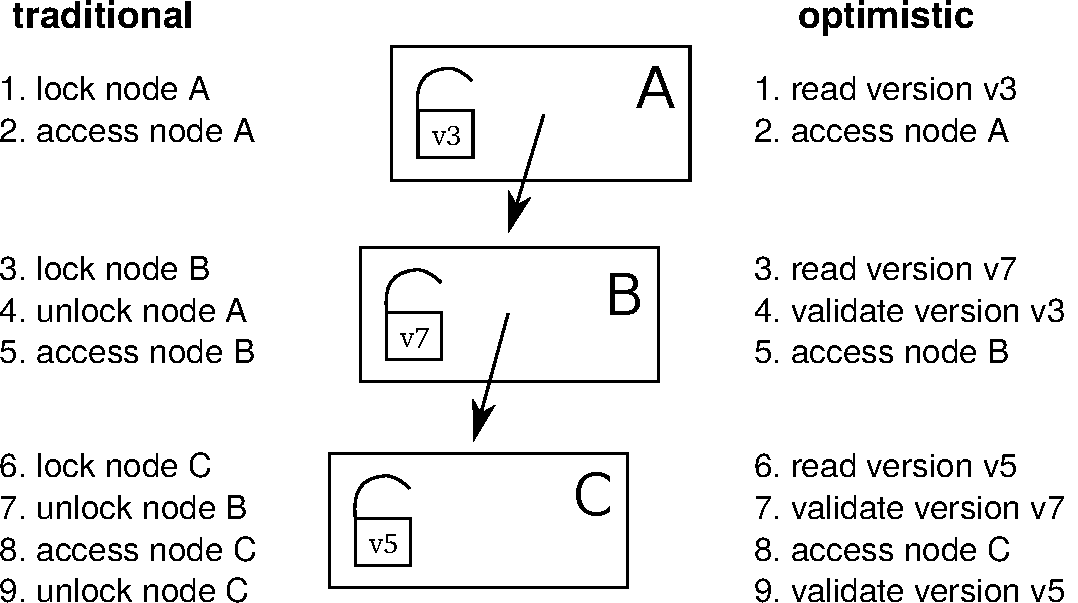
\includegraphics[width=0.65\linewidth]{olcall.pdf}
  \vspace{0.2cm}
  \caption{Comparison of a lookup operation in a 3-level tree using traditional lock coupling (left-hand side) vs.~optimistic lock coupling (right-hand side).}
  \label{fig:olc}
\end{figure}

The traditional and most common lock-based synchronization protocol for B-trees is lock coupling, which interleaves lock acquisitions while holding at most two locks at a time.
If, as we observed earlier, optimistic locks have similar semantics as traditional locks, it is natural to ask whether lock coupling can be combined with optimistic locks.
And indeed the answer is yes: One can almost mechanically translate traditional lock coupling code to optimistic lock coupling code.
This is illustrated in Figure~\ref{fig:olc}, which compares the traversal in a tree of height 3 using traditional and optimistic locks.
As the figure shows, the main difference is that locking is translated to reading the version and that unlocking becomes validation of the previously read version.
This simple change provides efficient lock-free tree traversal without the need to design a complex synchronization protocol.

It is important to emphasize the conceptual simplicity of OLC in comparison to data structures that use custom protocols like the Bw-tree~\cite{DBLP:conf/icde/LevandoskiLS13a}.
To implement lock-free access, the Bw-tree requires an indirection table, delta nodes, complex splitting and merging logic, retry logic, etc.
OLC, on the other hand, can directly be applied to B-trees mostly by adding the appropriate optimistic locking code and without modifying the node layout itself.
Therefore, OpenBw-Tree, an open source implementation of the Bw-tree, requires an order of magnitude more code than a B-tree based on OLC\footnote{Both implementations are available on GitHub: \url{https://github.com/wangziqi2016/index-microbench}}.
Given how difficult it is to develop, validate, and debug lock-free code, simplicity is obviously a major advantage.

\subsection{Correctness Aspects}

\begin{figure}
  % \centering
  %[basicstyle=\normalsize\ttfamily,showstringspaces=false,columns=fullflexible,breaklines=false,breakatwhitespace=true,numbers=none,numberstyle=\small,style=C,keepspaces=true]
\begin{lstlisting}[basicstyle=\ttfamily,language=C++,numbers=left,numberstyle=\small]
std::atomic<BTreeNode*> root;

// search for key in B+tree, returns payload in resultOut
bool lookup(Key key, Value& resultOut) {
   BTreeNode* node = root.load();
   uint64_t nodeVersion = node->readLockOrRestart();
   if (node != root.load()) // make sure the root is still the root
      restart();

   BTreeInner<Key>* parent = nullptr;
   uint64_t parentVersion = 0;

   while (node->isInner()) {
      auto inner = (BTreeInner*)node;

      // unlock parent and make current node the parent
      if (parent)
         parent->readUnlockOrRestart(parentVersion);
      parent = inner;
      parentVersion = nodeVersion;

      // search for next node
      node = inner->findChild(key);
      // validate 'inner' to ensure that 'node' pointer is valid
      inner->checkOrRestart(nodeVersion);
      // now it safe to dereference 'node' pointer (read its version)
      nodeVersion = node->readLockOrRestart();
   }

   // search in leaf and retrieve payload
   auto leaf = (BTreeLeaf*)node;
   bool success = leaf->findValue(key, resultOut);

   // unlock everything
   if (parent)
      parent->readUnlockOrRestart(parentVersion);
   node->readUnlockOrRestart(nodeVersion);

   return success;
}
\end{lstlisting}
  \vspace{0.2cm}
  \caption{B-tree lookup code using OLC. For simplicity, the restart logic is not shown.}
  \label{fig:lookup}
\end{figure}

So far, we have introduced the high-level ideas behind OLC and have stressed its similarity to traditional lock coupling.
Let us now discuss some cases where the close similarity between lock coupling and OLC breaks down.
To make this more concrete, we show the B-tree lookup code in Figure~\ref{fig:lookup}.
In the code, \texttt{readLockOrRestart} reads the lock version and \texttt{readUnlockOrRestart} validates that the read was correct.

One issue with OLC is that any pointer speculatively read from a node may point to invalid memory (if that node is modified concurrently).
Dereferencing such a pointer (e.g., to read its optimistic lock), may cause a segmentation fault or undefined behavior.
In the code shown in Figure~\ref{fig:lookup}, this problem is prevented by the extra check in line 25, which ensures that the read from the node containing the pointer was correct.
Without this additional validation, the code would in line 27 dereference the pointer speculatively read in line 23.
Note that the implementation of \texttt{checkOrRestart} is actually identical to \texttt{readUnlockOrRestart}.
We chose to give it a different name to highlight the fact that this extra check would not be necessary with read/write locks.

Another potential issue with optimistic locks is code that does not terminate.
Code that speculatively accesses a node, like an intra-node binary search, should be written in a way such that it always terminates---even in the presence of concurrent writes.
Otherwise, the validation code that detects the concurrent write will never run.
The binary search of a B-tree, for example, needs to be written in such a way that each comparison makes progress.
For some data structures that do not require loops in the traversal code (like ART) termination is trivially true.

\subsection{Implementation Details}

% implementation, efficiency
To implement an optimistic lock, one can combine the lock and the version counter into a single 64-bit\footnote{Even after subtracting one bit for the lock status, a back-of-the-envelope calculation can show that 63 bits are large enough to never overflow in practice.} word~\cite{artsync}.
A typical read operation will therefore merely consist of reading this version counter atomically.
In C++11 this can be implemented using the \texttt{std::atomic} type.

On x86, atomic reads are cheap because of x86's strong memory order guarantees.
No memory fences are required for sequentially-consistent loads, which are translated (by both GCC and clang) into standard \texttt{MOV} instructions.
Hence, the only effect of \texttt{std::atomic} for loads is preventing instruction re-ordering.
This makes version access and validation cheap.
Acquiring and releasing an optimistic lock in exclusive mode has comparable cost to a traditional lock:
A fairly expensive sequentially-consistent store is needed for acquiring a lock, while a standard \texttt{MOV} suffices for releasing it.
A simple sinlock-based implementation of optimistic locks can be found in the appendix of an earlier paper~\cite{artsync}.

OLC code must be able to handle restarts since validation or lock upgrade can fail due to concurrent writers.
Restarts can easily be implemented by wrapping the data structure operation in a loop (for simplicity not shown in Figure~\ref{fig:lookup}).
Such a loop also enables limiting the number of optimistic retry operations and falling back to pessimistic locking in cases of very heavy contention.
The ability to fall back to traditional locking is a major advantage of OLC in terms of robustness over lock-free approaches, which do not have this option.

In addition to the optimistic shared mode and the exclusive mode, optimistic locks also support a ``shared pessimistic'' mode, which physically acquires the lock in shared mode (allowing multiple concurrent readers but no writers).
This mode is useful for table (or range) scans that touch many tuples on a leaf page (which would otherwise easily abort).
Finally, let us mention that large range scans and table scans, should be broken up into several per-node traversals as is done in the LeanStore~\cite{leanstore} system.

Like all lock-free data structures, but unlike traditional locking and Hardware Transactional Memory~\cite{DBLP:conf/hpca/KarnagelDRLLSL14,DBLP:journals/pvldb/MakreshanskiLS15,htmtkde}, OLC requires care when deleting (and reusing) nodes.
The reason is that a deleting thread can never be sure that a node can be reclaimed because other threads might still be optimistically reading from that node.
Therefore, standard solutions like epoch-based reclamation~\cite{DBLP:conf/sosp/TuZKLM13}, hazard pointers~\cite{DBLP:journals/tpds/Michael04}, or optimized hazard pointers~\cite{DBLP:conf/spaa/BalmauGHZ16} need to be used.
These memory reclamation techniques are, however, largely orthogonal to the synchronization protocol itself.

%-lock-free is not a strong guarantee

\newpage
\section{Evaluation}\label{sec:evaluation}

Let us now experimentally evaluate the overhead and scalability of OLC.
For the experiments, we use an in-memory B+tree implemented in C++11 using templates, which is configured to use nodes of 4096 bytes, random 8 byte keys, and 8 byte payloads.
Based on this B-tree, we compare the following synchronization approaches:
\begin{itemize}
\item an OLC implementation\footnote{An almost identical OLC implementation is available on github: \url{https://github.com/wangziqi2016/index-microbench/tree/master/BTreeOLC}}
\item a variant based on traditional lock coupling and read/write locks
\item the unsynchronized B-tree, which obviously is only correct for read-only workloads but allows measuring the overhead of synchronization
\end{itemize}
Note that earlier work has compared the OLC implementation with a Bw-tree implementation~\cite{buzzword} and other state-of-the-art in-memory index structures.

We use a Haswell EP system with an Intel Xeon E5-2687W v3 CPU, which has 10 cores (20 ``Hyper-Threads'') and 25~MB of L3 cache.
The system is running Ubuntu 18.10 and we use GCC 8.2.0 to compile our code.
The CPU counters are obtained using the Linux perf API\footnote{We use the following convenience wrapper: \url{https://github.com/viktorleis/perfevent}}.

\begin{table}
  \caption{Performance and CPU counters for lookup and insert operations in a B-tree with 100M keys. We perform 100M operations and normalize the CPU counters by that number.}
  \label{tab:overhead}
  \centering
  \begin{tabular}{lrrrrrrr}\toprule
                    &         &        &        & instruc-  & L1     & L3     & branch \\
                    & threads & M op/s & cycles & tions & misses & misses & misses \\\midrule
lookup (no sync.)   & 1       & 1.72   & 2028   & 283     & 39.1   & 14.9   & 16.1   \\
lookup (OLC)        & 1       & 1.65   & 2107   & 370     & 43.9   & 15.1   & 16.7   \\
lookup (lock coup.) & 1       & 1.72   & 2078   & 365     & 42.3   & 16.9   & 15.7   \\\midrule
insert (no sync.)   & 1       & 1.51   & 2286   & 530     & 59.8   & 31.1   & 17.3   \\
insert (OLC)        & 1       & 1.50   & 2303   & 629     & 61.2   & 31.1   & 16.5   \\
insert (lock coup.) & 1       & 1.41   & 2473   & 644     & 61.0   & 31.0   & 17.2   \\\midrule
lookup (no sync.)   & 10      & 15.48  & 2058   & 283     & 38.6   & 15.5   & 16.0   \\
lookup (OLC)        & 10      & 14.60  & 2187   & 370     & 43.8   & 15.8   & 16.8   \\
lookup (lock coup.) & 10      & 5.71   & 5591   & 379     & 54.2   & 17.0   & 14.8   \\\midrule
insert (no sync.)   & 10      & -      & -      & -       & -      & -      & -      \\
insert (OLC)        & 10      & 10.46  & 2940   & 656     & 62.0   & 32.5   & 16.8   \\
insert (lock coup.) & 10      & 7.55   & 4161   & 667     & 75.0   & 28.6   & 16.2   \\
    \bottomrule
\end{tabular}
\end{table}

Table~\ref{tab:overhead} compares the performance and CPU counters for lookup and insert operations in a B-tree with 100M keys.
With {\em single-threaded} execution, we observe that all three approaches have very similar performance.
Adding traditional or optimistic locks to unsynchronized B-tree code results in up to 30\% of additional instructions without affecting single-threaded performance much.

\begin{figure}
  \centering
  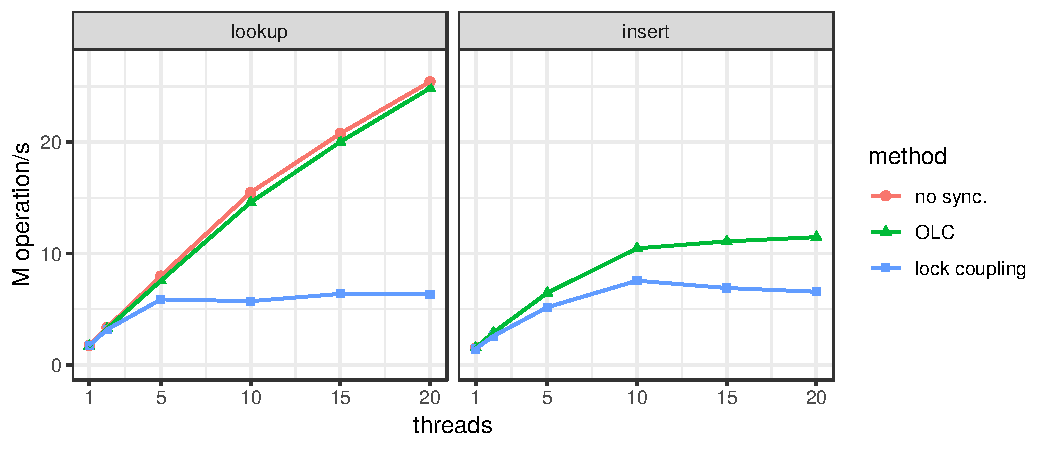
\includegraphics[width=\linewidth]{scale.pdf}
  \vspace{0.2cm}
  \caption{Scalability on 10-core system for B-tree operations (100M values).}
  \label{fig:scale}
\end{figure}

As Figure~\ref{fig:scale} shows, the results change dramatically once we use multiple threads.
For lookup, the scalability of OLC is near-linear up to 20 threads, even though the system has only 10 ``real cores''.
The OLC scalability for insert is also respectable (though not quite as linear because multi-threaded insertion approaches the memory bandwidth of our processor).
The figure also shows that the results of traditional lock coupling with read/write locks are significantly worse than OLC.
With 20 threads, lookup with OLC is 3.9$\times$ faster than traditional lock coupling.

\section{Summary}\label{sec:conc}

Optimistic Lock Coupling (OLC) is an effective synchronization method that combines the simplicity of traditional lock coupling with the superior scalability of lock-free approaches.
OLC is widely applicable and has already been successfully used to synchronize several data structures, including B-trees, binary search trees, and different trie variants.
These features make it highly attractive for modern database systems as well as performance-critical systems software in general.

\begin{thebibliography}{10}

\bibitem{DBLP:conf/spaa/BalmauGHZ16}
O.~Balmau, R.~Guerraoui, M.~Herlihy, and I.~Zablotchi.
\newblock Fast and robust memory reclamation for concurrent data structures.
\newblock In {\em SPAA}, 2016.

\bibitem{DBLP:journals/acta/BayerS77}
R.~Bayer and M.~Schkolnick.
\newblock Concurrency of operations on {B}-trees.
\newblock {\em Acta Informatica}, 9, 1977.

\bibitem{hot}
R.~Binna, E.~Zangerle, M.~Pichl, G.~Specht, and V.~Leis.
\newblock {HOT}: A height optimized trie index for main-memory database
  systems.
\newblock In {\em SIGMOD}, 2018.

\bibitem{DBLP:conf/ppopp/BronsonCCO10}
N.~G. Bronson, J.~Casper, H.~Chafi, and K.~Olukotun.
\newblock A practical concurrent binary search tree.
\newblock In {\em PPOPP}, 2010.

\bibitem{DBLP:conf/vldb/ChaHKK01}
S.~K. Cha, S.~Hwang, K.~Kim, and K.~Kwon.
\newblock Cache-conscious concurrency control of main-memory indexes on
  shared-memory multiprocessor systems.
\newblock In {\em VLDB}, 2001.

\bibitem{intel}
I.~Cutress.
\newblock {Intel} goes for 48-cores: {Cascade-AP} with multi-chip package
  coming soon.
\newblock
  \url{https://www.anandtech.com/show/13535/intel-goes-for-48cores-cascade-ap},
  2018 (accessed January, 2019).

\bibitem{DBLP:conf/cidr/FaleiroA17}
J.~M. Faleiro and D.~J. Abadi.
\newblock Latch-free synchronization in database systems: Silver bullet or
  fool's gold?
\newblock In {\em CIDR}, 2017.

\bibitem{DBLP:journals/ftdb/Graefe11}
G.~Graefe.
\newblock Modern {B}-tree techniques.
\newblock {\em Foundations and Trends in Databases}, 3(4), 2011.

\bibitem{DBLP:conf/hpca/KarnagelDRLLSL14}
T.~Karnagel, R.~Dementiev, R.~Rajwar, K.~Lai, T.~Legler, B.~Schlegel, and
  W.~Lehner.
\newblock Improving in-memory database index performance with
  {Intel}\({}^{\mbox{{\textregistered}}}\) transactional synchronization
  extensions.
\newblock In {\em HPCA}, 2014.

\bibitem{DBLP:journals/tods/LehmanY81}
P.~L. Lehman and S.~B. Yao.
\newblock Efficient locking for concurrent operations on {B}-trees.
\newblock {\em {ACM} Trans. Database Syst.}, 6(4), 1981.

\bibitem{leanstore}
V.~Leis, M.~Haubenschild, A.~Kemper, and T.~Neumann.
\newblock Leanstore: In-memory data management beyond main memory.
\newblock In {\em ICDE}, 2018.

\bibitem{art}
V.~Leis, A.~Kemper, and T.~Neumann.
\newblock The adaptive radix tree: {ARTful} indexing for main-memory databases.
\newblock In {\em ICDE}, 2013.

\bibitem{htmtkde}
V.~Leis, A.~Kemper, and T.~Neumann.
\newblock Scaling {HTM}-supported database transactions to many cores.
\newblock {\em {IEEE} Trans. Knowl. Data Eng.}, 28(2), 2016.

\bibitem{artsync}
V.~Leis, F.~Scheibner, A.~Kemper, and T.~Neumann.
\newblock The {ART} of practical synchronization.
\newblock In {\em DaMoN}, 2016.

\bibitem{DBLP:conf/icde/LevandoskiLS13a}
J.~J. Levandoski, D.~B. Lomet, and S.~Sengupta.
\newblock The {Bw}-tree: A {B}-tree for new hardware platforms.
\newblock In {\em ICDE}, 2013.

\bibitem{DBLP:journals/pvldb/MakreshanskiLS15}
D.~Makreshanski, J.~J. Levandoski, and R.~Stutsman.
\newblock To lock, swap, or elide: On the interplay of hardware transactional
  memory and lock-free indexing.
\newblock {\em {PVLDB}}, 8(11), 2015.

\bibitem{DBLP:dblp_conf/eurosys/MaoKM12}
Y.~Mao, E.~Kohler, and R.~T. Morris.
\newblock Cache craftiness for fast multicore key-value storage.
\newblock In {\em EuroSys}, 2012.

\bibitem{DBLP:journals/tpds/Michael04}
M.~M. Michael.
\newblock Hazard pointers: Safe memory reclamation for lock-free objects.
\newblock {\em {IEEE} Trans. Parallel Distrib. Syst.}, 15(6), 2004.

\bibitem{DBLP:journals/jacm/ShalevS06}
O.~Shalev and N.~Shavit.
\newblock Split-ordered lists: Lock-free extensible hash tables.
\newblock {\em J. {ACM}}, 53(3), 2006.

\bibitem{amd}
A.~Shilov.
\newblock {AMD} previews {EPYC} ‘{Rome}’ processor: Up to 64 {Zen} 2 cores.
\newblock
  \url{https://www.anandtech.com/show/13561/amd-previews-epyc-rome-processor-up-to-64-zen-2-cores},
  2018 (accessed January, 2019).

\bibitem{DBLP:conf/sosp/TuZKLM13}
S.~Tu, W.~Zheng, E.~Kohler, B.~Liskov, and S.~Madden.
\newblock Speedy transactions in multicore in-memory databases.
\newblock In {\em SOSP}, 2013.

\bibitem{buzzword}
Z.~Wang, A.~Pavlo, H.~Lim, V.~Leis, H.~Zhang, M.~Kaminsky, and D.~Andersen.
\newblock Building a {Bw}-tree takes more than just buzz words.
\newblock In {\em SIGMOD}, 2018.

\end{thebibliography}


%\bibliographystyle{abbrv}
%\bibliography{main}

\end{document}

\end{article}


\begin{article}
{Fairness in Practice: A Survey on Equity in Urban Mobility}
{An Yan, Bill Howe}
\graphicspath{{submissions/Howe/}}
\documentclass[11pt]{article}
% \usepackage[utf8]{inputenc}
\usepackage{deauthor,times,graphicx}
\usepackage{enumitem}
% \setlist{nolistsep,leftmargin=*}

%%%% macros.tex

%\usepackage{anysize}
%\usepackage{geometry}
%\geometry{top=1in, left=1in, right=1in, bottom=1in,footskip=.25in}
%\marginsize{1in}{0.8in}{1in}{1in}%tblr
%\usepackage[showframe,bottom=0.2in,footskip=.25in]{geometry}
%\usepackage[left=1in, right=1in, top=1in]{geometry}
%\newcommand{\cmt}[2]{\textcolor{dkmag}{[#1: #2]}}
%\newcommand{\personname}[1]{\cmt{Personname}{#1}}
%\newcommand{\standout}[1]{\textit{\textcolor{dkmag}{#1}}}
%usepackage[T1]{fontenc}
%\usepackage{fontspec}
%\setmainfont[Scale=0.85, Ligatures={Required,Common,Contextual,TeX}]{TeX Gyre Schola} % Incredible font inside latex

%
%\usepackage{fancyhdr}
%\usepackage{fullpage} %, hyperref}
%\usepackage{amssymb, amsmath, enumitem, titling, hyperref}
%\usepackage[standard]{ntheorem}
%%\usepackage[sort&compress]{natbib}
%\usepackage[top=0.65in, bottom=1.2in, left=0.95in, right=0.95in]{geometry}
% %\ifthenelse{\value{page}=1}
%          %{\setlength\headheight{40pt}}
%          %{\setlength\headheight{0pt}}
%
%\usepackage[backend=bibtex,sorting=anyt, maxnames=7, firstinits=true]{biblatex} %hyperref=true,
%\renewcommand*{\bibfont}{\footnotesize}
%\bibliography{bib_rs}
%%\renewcommand{\baselinestretch}{0.9}
\usepackage{multirow}
\usepackage{float}
\usepackage{caption}
%\usepackage{subfloat}
%\usepackage{float}
\usepackage{amsmath}
\usepackage{graphicx, multicol, latexsym, amsmath, amssymb}
\usepackage{blindtext}
\usepackage{caption}
\def\sharedaffiliation{%
\end{tabular}
\begin{tabular}{c}}
\newcommand{\vset}[1]{\mathbf{#1}}
%\usepackage{amsthm}
%
%\theoremstyle{definition}
%\newtheorem{definition}{Definition}[section]
% end Spencer

\newcommand{\reva}[1]{{ { { #1}}}}
\newcommand{\revb}[1]{{{ { #1}}}}
\newcommand{\revc}[1]{{{{ #1}}}}
\newcommand{\revd}[1]{{{{ #1}}}}
\newcommand{\reve}[1]{{{ { #1}}}}
%\newcommand{\revf}[1]{{{\color{red} {#1}}}}




\newcommand{\mypm}{\mathbin{\tikz [x=1.4ex,y=1.4ex,line width=.1ex] \draw (0.0,0) -- (1.0,0) (0.5,0.08) -- (0.5,0.92) (0.0,0.5) -- (1.0,0.5);}}%


\newcommand{\qii}{\delta}

\newcommand{\createcontingencytable}[4]{ %
	% #1=table name
	% #2=first column name
	% #3=new row sum name
	% #4=new column sum name
	\pgfplotstablecreatecol[
	create col/assign/.code={% In each row ...
		\def\rowsum{0}
		\pgfmathtruncatemacro\maxcolindex{\pgfplotstablecols-1}
		% ... loop over all columns, summing up the elements
		\pgfplotsforeachungrouped \col in {1,...,\maxcolindex}{
			\pgfmathsetmacro\rowsum{\rowsum+\thisrowno{\col}}
		}
		\pgfkeyslet{/pgfplots/table/create col/next content}\rowsum
	}
	]{#3}{#1}%
	%
	% Transpose the table, so we can repeat the summation step for the columns
	\pgfplotstabletranspose[colnames from={#2},input colnames to={#2}]{\intermediatetable}{#1}
	%
	% Sums for each column
	\pgfplotstablecreatecol[
	create col/assign/.code={%
		\def\colsum{0}
		\pgfmathtruncatemacro\maxcolindex{\pgfplotstablecols-1}
		\pgfplotsforeachungrouped \col in {1,...,\maxcolindex}{
			\pgfmathsetmacro\colsum{\colsum+\thisrowno{\col}}
		}
		\pgfkeyslet{/pgfplots/table/create col/next content}\colsum
	}
	]{#4}\intermediatetable
	%
	% Transpose back to the original form
	\pgfplotstabletranspose[colnames from=#2, input colnames to=#2]{\contingencytable}{\intermediatetable}
}
%

% \PassOptionsToPackage{hyphens}{url}\usepackage{hyperref}
\newcommand{\inp}{{{\mb X }}}
\newcommand{\cm}{{{\mb M }}}
\newcommand{\acm}{{{\mb M_{\mc A} }}}
\newcommand{\cg}{ G}
\newcommand{\acg}{ G_{\mb M_{\mc A}} }

\newcommand{\nipsadult}{{{Binned Adult}}}
\newcommand{\nipscompas}{{{Binned COMPAS}}}
\usepackage{booktabs,siunitx}
% \DeclareMathOperator*{\argmax}{argmax}
% \DeclareMathOperator*{\argmin}{argmin}
\newcommand{\fge}{{\bf {FGE}}}
\newcommand{\scmit}{{\bf {SNMIT}}}
\newcommand{\cmit}{{\bf {MIT}}}
\newcommand{\icmit}{{\bf {FNMIT}}}
\newcommand{\iscmit}{{\bf {FMIT}}}
\newcommand{\hcmit}{{\bf {HyMIT}}}
\newcommand{\ogsal}{{\bf {OGS}}}
\newcommand{\gsal}{{\bf {GS}}}
\newcommand{\pdal}{{\bf {CD}}}
\newcommand{\delay}{{\tt \textsc{Flight Delay}}}
\newcommand{\ate}{{\tt \textsc{ATE}}}
\newcommand{\nde}{{\tt \textsc{NDE}}}
\newcommand{\nie}{{\tt \textsc{NIE}}}
\newcommand{\E}{{\tt \mathbb{E}}}
\newcommand{\pr}{{\tt \mathrm{Pr}}}
\newcommand{\hsys}{{\textsc{HypDB}}}
\newcommand{\sys}{{\textsc{Capuchin}}}
\newcommand{\dal}{{{SGS}}}
\newcommand{\bigCI}{\mathrel{\text{\scalebox{1.07}{$\perp\mkern-10mu\perp$}}}}
\newcommand{\nbigCI}{\cancel{\mathrel{\text{\scalebox{1.07}{$\perp\mkern-10mu\perp$}}}}}
\newcommand{\rred}[1]{\textcolor{red}{#1}}
\newcommand{\mc}[1]{\mathcal{#1}}
\newcommand{\ind}[0]{\textrm{Indep}}
\newcommand{\ignore}[1]{}
\newcommand{\comlb}[1]{{\vspace{2mm}\noindent \rred{\bf COMM(Dan):}}~ #1 \hfill {\bf    END.}\\}
\newcommand{\combabak}[1]{{\vspace{4mm}\noindent \bf  COMM(Babak):}~ {\em \rred{#1}}\hfill {\bf END.}\\}



\newcommand*{\rom}[1]{\expandafter\@slowromancap\romannumeral #1@}

\newcommand{\dan}[1]{{{\color{red} {\bf\underline{Dan}}: [{#1}]}}}
\newcommand{\babak}[1]{{\texttt{\color{red} Babak: [{#1}]}}}
\newcommand{\bill}[1]{{\texttt{\color{olive} Bill: [{#1}]}}}
\newcommand{\luke}[1]{{\texttt{\color{blue} Luke: [{#1}]}}}
\newcommand{\johannes}[1]{{\texttt{\color{blue} Johannes: [{#1}]}}}
\newcommand{\red}[1]{{\textbf {{\color{red} [{#1}]}}}}
\newcommand{\scream}[1]{{\texttt{\color{red}{\textbf{[{#1}]}}}}}

\newcommand{\LOGSPACE}{{\scriptsize $  \mathrm{LOGSPACE}$}}
\newcommand{\NLOGSPACE}{{\scriptsize $  \mathrm{NLOGSPACE}$}}
\newcommand{\PTIME}{{\scriptsize $  \mathrm{PTIME}$ }}
\newcommand{\nindep}{\mbox{$\not\!\perp\!\!\!\perp$}}
\newcommand{\indep}{\mbox{$\perp\!\!\!\perp$}}





\newcommand{\tr}{1} %{\mathtt{t}}
\newcommand{\cn}{0} %{\mathtt{c}}

%infotheo
\newcommand{\rep}{D'}
\newcommand{\icq}{Q_\varphi}
\newcommand{\hb}{D^*}


\newcommand{\satt}{\mathbf{a}}
\newcommand{\att}{\mathbf{A}}
\newcommand{\sx}{\mathbf{x}}
\newcommand{\bx}{\mathbf{X}}
\newcommand{\pn}{\textmd{N}}
\newcommand{\ent}{{\mathcal{H}}}
\newcommand{\minf}{{{I}}}
\newcommand\mvd{\twoheadrightarrow}
\newcommand{\amvd}{\twoheadrightarrow_\alpha}
\newcommand{\fd}{\rightarrow}
\newcommand{\afd}{\rightarrow_\alpha}
\newcommand{\bfd}{\rightarrow_\beta}
\newcommand{\abfd}{\rightarrow_{\alpha+\beta}}
\newcommand{\A}{\texttt{A}}
\newcommand{\K}{\texttt{K}}
\newcommand{\deletelater}[1]{{\textbf {{\color{green} [{#1}]}}}}
\newcommand{\intervrel}{\texttt{intervened-relation}}

\newcommand{\annot}{\texttt{annot}}
\newcommand{\supp}{\texttt{supp}}
\newcommand{\sch}{{\mathcal{S}}}
\newcommand{\rel}{{\mathcal{R}}}
%\newcommand{\interv}{{\Gamma}}
\newcommand{\real}{{\mathbb{R}}}
\newcommand{\nat}{{\mathbb{N}}}
\newcommand{\explattr}{{\{E\}}}
%\newcommand{\change}{{\Delta}}
\newcommand{\bool}{{\textit{b}}}


\newcommand{\AP}{\texttt{AP}}
\newcommand{\highval}{\texttt{high}}
\newcommand{\midval}{\texttt{mid}}
\newcommand{\lowval}{\texttt{low}}
\newcommand{\aplow}{\texttt{poor}}
\newcommand{\aphigh}{\texttt{good}}
\newcommand{\dbnull}{\texttt{null}}
\newcommand{\relset}{\mathcal{R}}
\newcommand{\reltop}{{\mathcal{R}}_{top}}
\newcommand{\relbot}{{\mathcal{R}}_{bot}}
\newcommand{\attrset}{\mathcal{A}}
\newcommand{\attrtop}[1]{{\mathcal{A}}_{{top}, {#1}}}
\newcommand{\attrbot}{{\mathcal{A}}_{bot}}
%\newcommand{\featureset}{\mathcal{B}}
\newcommand{\wcl}{\mathscr{C}(\mb{C})}
\newcommand{\rwq}{{ {\mc{Q}_{rw}}}}
\newcommand{\db}{{D}}
\newcommand{\dbdom}{\mathbf{DB}}
\newcommand{\intervadditive}{{intervention-additive}}
\newcommand{\val}{{v}}
\newcommand{\valorig}{{u}}
%\newcommand{\dbdom}{\mathcal{D}}
\newcommand{\inputclass}{\mathcal{C}}
%\newcommand{\intervene}{\mathcal{I}}
%\newcommand{\tbaff}{{\tt{T_{Aff}}}}
%\newcommand{\attaff}{{\tt{A_{Aff}}}}
\newcommand{\univ}{{{U}}}
\newcommand{\pk}{{\mathtt{pk}}}
\newcommand{\fk}{{\mathtt{fk}}}
\newcommand{\expl}{{\phi}}
%\newcommand{\pk}{{\tt \mathtt{\pk}}}
\newcommand{\sign}{{\tt \mathtt{sign}}}
%\newcommand{\expldom}{{\Phi}}

\newcommand{\select}{\tt {\textsc{Select}}}
\newcommand{\where}{{\tt \textsc{Where}}}
\newcommand{\with}{{\tt \textsc{With}}}
\newcommand{\distinct}{{\tt \textsc{distinct}}}
\newcommand{\groupby}{{\tt \textsc{Group By}}}
\newcommand{\from}{{\tt \textsc{From}}}
\newcommand{\ct}{{\tt \textsc{Count}}}
\newcommand{\create}{{\tt \textsc{Create}}}
\newcommand{\explanation}{{\tt \textsc{Explanation}}}
%\newcommand{\Pr}{{\tt {Pr}}}
\newcommand{\on}{{\tt \textsc{On}}}
\newcommand{\sqlwith}{{\tt \textsc{With}}}
\newcommand{\as}{{\tt \textsc{as}}}
\newcommand{\cascade}{{\tt \textsc{Cascade}}}
\newcommand{\sqland}{{\tt \textsc{And}}}
\newcommand{\sqlin}{{\tt \textsc{In}}}
\newcommand{\true}{{\tt true}}
\newcommand{\false}{{\tt false}}
\newcommand{\inmath}[1]{{\mathtt {#1}}}

\newcommand{\RNum}[1]{\uppercase\expandafter{\romannumeral #1\relax}}
\newcommand{\ie}{{\em i.e.}} %\xspace}
\newcommand{\eg}{{\em e.g.}} %\xspace}
\newcommand{\etal}{{et al.}} %\xspace}
\newcommand{\aka}{{\em a.k.a.}\xspace}
\newcommand{\algorithmicbreak}{\textbf{Break}}
\newcommand{\backwd}{\mathcal{B}}
\newcommand{\mbl}{{\bf B}}
\newcommand{\mmb}{{\bf MB}}
\newcommand{\emb}{{ \bf MB}_\epsilon}
\newcommand{\embl}{{\bf B}_\epsilon}
\newcommand{\emmb}{{\bf IB}_{(\epsilon,\beta)}}
\newcounter{enumQues}
\newcommand{\mf}[1]{\mathrm{\mathfrak{#1}}}
\newcommand{\mb}[1]{{\mathbf{#1}}}
\newtheorem{defn}{Definition}[section]
\newtheorem{rem}[defn]{Remark}
\newtheorem{conj}[defn]{Conjecture}
\newtheorem{prop}[defn]{Proposition}
\newtheorem{obs}[defn]{Observation}
\newtheorem{assumption}[defn]{Assumption}
\newcommand{\proj}[1]{{\Pi}}
\newcommand{\sel}[1]{{\sigma}}

\newcommand{\un}[1]{{\underline{#1}}}
\newcommand{\ov}[1]{{\overline{#1}}}
\newcommand{\cut}[1]{}
\newcommand{\eat}[1]{}

\newcommand{\causalframework}{interventional fairness}
\newcommand{\metric}{interventional discrimination}
\newcommand{\fairalgorithm}{interventional fairness}

\newcommand{\defeq}{\stackrel{\text{def}}{=}}

\newcommand{\fairapp}{fairness application~}

\newcommand\blfootnote[1]{%
  \begingroup
  \renewcommand\thefootnote{}\footnote{#1}%
  \addtocounter{footnote}{-1}%
  \endgroup
}




%%%%%%%%%%%


\graphicspath{{submissions/Howe/}}

\begin{document}
\title{Fairness in Practice: A Survey on Equity in Urban Mobility} 


\author{An Yan, \  Bill Howe \\
University of Washington\\
\{yanan15,billhowe\}@uw.edu}

\maketitle
\blfootnote{This work is supported by the National Science Foundation under grant NSF BIGDATA-1740996.}

\section{Introduction}
More than 54 percent of the world's population lives in urban areas \cite{zhang2017regions}. Predicting dynamic urban activities such as energy consumption, air pollution, public safety, and traffic flows has become a fundamental task for improving the quality of human life. Urban mobility is closely intertwined with these problems, and is therefore a major determinant of quality of life \cite{shafrin2017association}, crucial to employment opportunities and access to resources such as education and health care \cite{chan2016screening}. %Prediction tasks for urban mobility include transport resource demand prediction, travel time prediction, traffic flows prediction, ride-hailing waiting time estimation, and behavior analysis for autonmous vehicles. 

Evidence suggests that residents of low-income and minority neighborhoods are concentrated away from economic opportunity and public resources \cite{wang2018urban}. Injustice of transportation services experienced by these residents further reinforces social exclusion as the availability and quality of transportation impact a person’s access to opportunities \cite{litman2018evaluating, shaheen2017travel, palmateer2017justice, ricciardi2015exploring}. For example, one study revealed that living in neighborhoods with longer commute times is associated with lower employment rates of younger generations \cite{chetty2016childhood}. As a result, transportation equity issues have motivated government agencies to develop extensive multimodal transportation networks\cite{shaheen2017travel}. 

\textit{New mobility }is about emerging transportation modes, including but not limited to car-sharing, bike-sharing, and ride-hailing or Transportation Network Companies (TNCs) \cite{goldman2006sustainable}. New mobility services provide technology-based, on-demand, and affordable alternatives to traditional means. These services offer a chance to address persistent equity issues in transportation. However, new mobility services also bring new equity concerns. For example, people without internet service, smart phones, or credit cards are not able to get access to the services. Moreover, studies show that algorithms or human beings that distribute app-based mobility services may discriminate against people of color \cite{ge2016racial}. 
%Although a line of equity research has been developed to  focus on new mobility systems, the equity implications of them are not well understood. 

This paper reviews the methods and findings of mobility equity studies, with a focus on new mobility. The paper is structured as follows: Section \ref{sec:headings} presents the background of transportation equity. Section 3 summarizes the main findings from current equity studies for mobility systems, with a brief discussion on future research. Section 4 reviews the commonly used methods for evaluating the equity of mobility service provision and usage and considers strengths and weaknesses.  Section 5 discusses the relationship between the transportation equity community and the fairness in machine learning community. Section 6 concludes the paper. 


% Modern scientific methods including hypothesis testing, computer simulation, process-based models, and machine learning have witnessed success in tacking urban challenges in the past decades [cite].  Recent advances of deep learning, and the growing availability of urban data offer exciting challenges opportunities for extending our capability to model the spatio-temporal dynamics of urban events from data with exceptional accuracy. Among the many aspects of urban events, this paper focuses on mobility and reviews the state of the art deep learning methods for forecasting urban mobility events. 

% Urban mobility, an important aspect of urban  is about how people move around the city using common transport means such as walking, cycling, public transport, car, or motorcycle [Vasconcellos, 2018]. 

% New mobility is an emerging transportation system currently features car-sharing, ride-hailing, and bike-sharing. It is technology-enabled, seamless, and on-demand. 

% Examples of prediction tasks for new mobility include bike / ride-hailing demand prediction, ride-hailing waiting time estimation, and driving behavior analysis for automatic driving cars. 


\section{Equity in Mobility Systems: Background}
\label{sec:headings}

Automated decision systems powered by machine learning and big data have been widely employed in many applications including credit scoring, criminal justice, online advertising, employment, etc \cite{zliobaite2015survey,petrasic2017algorithms, miller2015algorithms, rudin2013predictive}. These systems have been hailed as efficient, objective, and accurate alternatives to human decision makers \cite{barocas2017fairness}. However, increasing evidence has shown that data-driven systems contain biases. For example, Google’s image recognition system wrongly identified black users as gorillas \cite{guynn2015google}. Amazon’s same-day delivery services excluded predominantly black neighborhoods in many cities to a varying degree \cite{ingold2016amazon}. 

Even if the algorithms themselves are well-intentioned, they can replicate and amplify human biases encoded in the data, thus resulting in unequal distribution of impacts across different demographic groups \cite{zliobaite2015survey, lepri2017tyranny, barocas2016big}. This effect is due to machine learning algorithms seeking to fit the training data as closely as possible to make accurate predictions. The process of learning also “accurately” captures historical signals of discrimination. In 2017, Caliskan et al. \cite{caliskan2017semantics} found that an influential language corpus \cite{pennington2014glove} generated by machine learning algorithms accurately reproduced historic biases. The corpus reflects societal stereotypes such as female names are more associated with family while male names are more associated with career. Not only do algorithms pick up discrimination in data, they also magnify them \cite{chouldechova2018frontiers}. This effect is often due to the underrepresentation of minority groups in training data, leading to higher error rates for the minorities. One study \cite{lum2016predict} revealed that a widely-used predictive policing tool, PredPol, would reinforce the bias in the police-recorded, resulting in disproportionate policing of minority communities. 

The heightened concerns about automated decision systems concentrate not only on discrimination, but also on a range of related issues, including transparency, privacy, and accountability \cite{young2019beyond}. These issues often intertwine and conflict with one another in practice. In the context of automatic decision systems, transparency is about the openness and understandability of data and models and accountability is about being responsible for the decisions \cite{lepri2018fair}. Transparency is a critical prerequisite for accountability. In the absence of concrete evidence of intentional discrimination, it is difficult to hold an individual or organization accountable for biased decisions. 

In practice, transparency for automatic decision systems is not easily achievable. Burrell \cite{burrell2016machine} summarized three types of barriers to transparency: 1) intrinsic opacity, where some algorithms such as deep learning models are difficult to understand and interpret; 2) illiterate opacity, which says the general public may lack the expertise to understand the algorithms; and 3) intentional opacity, which is often resulted from intellectual property protection of the algorithm developers. 
%In the Amazon same-day delivery case, white residents were more than twice as likely to live in service areas than black residents in several cities \cite{ingold2016amazon}. The demographic disparities are striking, but we do not have evidence to show that race is part of Amazon’s decision making, because the decision making process is not transparent. Companies like Amazon rarely disclose key technical information for fear of exposing trade secrets and losing competitive advantages. It is thus impossible to further pursue this case to find out the causes of discrimination \cite{diakopoulos2016accountability}.

\subsection{Definitions of transportation equity}
Equity in the context of mobility has been studied independently since well before the recent interest in generalized fairness methods for machine learning.  These efforts suggest that domain-specific and context-sensitive approaches should be incorporated into any fairness-aware ML system.  Equity for mobility is the fair distribution of transportation costs and benefits, among current (and future) members of society \cite{litman2018evaluating}. 

There are mainly two perspectives from which to examine equity: horizontal equity and vertical equity. \textit{Horizontal equity} (also called fairness and egalitarianism) is concerned with providing equal resources to individual or groups considered equal in ability and need, which means the public policies avoid favoring one individual or group over another. Horizontal equity suggests that those who pay more should receive superior services. 

\textit{Vertical equity} (also referred to as social justice, environmental justice, and social inclusion) is concerned with allocating resources to individuals or groups that differ in income, social class, mobility need, or ability.  It advocates that public policies favor disadvantaged groups by providing discounts or special services, therefore compensating for overall inequities. One way to evaluate vertical equity is \textit{equity of opportunity}, meaning that disadvantaged groups should have adequate access to transportation resources. Equity of opportunity is usually measured by access to services. In contrast, “\textit{equity of outcome}” is usually measured by the actual usage of the systems across groups. There is a general agreement about the goal of equity of opportunity, but less agreement about equity of outcome \cite{litman2018evaluating, delbosc2011using,lucas2016method}. 

There are other ways to define transportation equity. Social equity indicates the differences between socioeconomic groups. Spatial equity refers to the differences in transport services among geographic regions \cite{feng2014trade}. These different definitions often overlap or conflict with each other. For example, horizontal equity requires the users to pay for what they get, whereas vertical equity prioritizes the needs of disadvantaged groups such as the low-income or ethnic minorities in the form of discounts \cite{thomopoulos2009incorporating}.

% \subsubsection{Relationship to fairness notions in machine learning community}
% In examining the fairness (equity) definitions from transportation community and machine learning community, I observe that a natural mapping between them can be established, though further effort is needed to create a consistent mapping between concepts in one domain to the other. \textit{Horizontal equity} echoes the spirit of \textit{individual fairness} (similar people should be treated similarly). \textit{Vertical equity} roughly corresponds to \textit{group fairness} (sensitive attributes should be independent from outcomes). This is true in cities where there is an uneven distribution of transport supply across different socioeconomic groups. Vertical equity encourages compensating for such inequalities by policies favoring disadvantaged groups. This aligns with group fairness that the level of transportation supply in a city should be the same across different groups. Vertical equity and group fairness are only "roughly" related because by definition, group fairness stresses "independence" between sensitive attributes and outcome, whereas vertical equity does not.   

\subsection{Evaluation of mobility equity}

Mobility equity research addresses a wide range of issues, including, for example, economic studies on how transportation is subsidized and taxed, and operational studies on how negative impacts of transportation systems are distributed among different groups \cite{shaheen2017travel}. Litman \cite{litman2018evaluating} proposed four variables to consider when performing any equity evaluation.
\begin{itemize}
\item Type of equity: horizontal equity or vertical equity
\item Impact (costs and benefits) categories: public facilities and services, user costs and benefits (e.g., taxes and fares), service quality (e.g., public transportation service quality including frequency, speed, safety, reliability, comfort, etc.), external impacts (e.g., air pollution), economic impacts (e.g., access to employment), and regulation and enforcement (e.g., parking regulations)
\item Measurement unit: per capita, per unit of travel (e.g., per trip), or per dollar. 
\item Categorization of people: demographics (e.g., age, household type, race), income class, ability, location, mode (e.g., pedestrians, public transit), industry (e.g., freight, public transit), and trip type (e.g., commutes)
\end{itemize}

This paper focuses on the equity of new mobility systems service provision and usage across different social-economic, demographic, or geographic groups. 


\section{Findings from Equity Research in Mobility Systems}
\label{sec:others}
We describe findings in the literature across 1) public transportation, and 2) new mobility services.

\paragraph{Public transportation}

Transportation equity has long been a major concern of governmental agencies, researchers, and the general public \cite{litman2018evaluating, shaheen2017travel, palmateer2017justice}. Despite the tremendous investment in transportation system development and progress in transportation equity research, there are still many long-standing equity issues resulted from unequal distributions of transport resources across different socioeconomic groups and spatial regions \cite{raphael2002car, bullard2003addressing, ricciardi2015exploring, el2016cost}. A number of studies have found out that an uneven urban development has resulted in a lack of public transport supply for disadvantaged groups.  For example, Vasconcellos \cite{vasconcellos2018urban} pointed out in Brazil, road systems are developed in a radial pattern. Low-income residents usually settled in fringes of the city with irregular pavements or hilly areas that are subject to landslides. The urban centers with good public services are mostly occupied by the high-income people.  Similarly, Ricciardi \cite{ricciardi2015exploring} found that there is an unequal spatial distribution of public transport resources in two Australian cities. Their analysis showed that 70\% of Perth’s population shares one third of the public transit supply. Moreover, three socially disadvantaged groups --– the elderly, low-income, and no-car households have less access to public transport services compared to the overall population. Some studies also showed that the economic burden and negative climate impacts of transportation systems is disproportionately imposed on disadvantaged people \cite{bullard2003addressing, feng2014trade, cohen2017framework}. In recognizing these issues, many cities now have incorporated social equity into urban transportation planning. However, one study found that social equity goals are often not translated into clear and actionable items and there is a lack of appropriate methods for assessing their achievements \cite{manaugh2015integrating, litman2018evaluating}. Current literature on equity in public transport suggests that disadvantaged groups as a whole experience inequitable access to public transport services but suffer from significant negative impacts from the transportation systems. 
%Further development of transportation systems and policies are needed to overcome these issues. 

\subsection{New mobility}
\paragraph{Bikeshare} A number of researchers have studied equity in bikeshare systems. Several studies found that bikeshare stations were typically located in urban centers with high population density \cite{ogilvie2012inequalities, meng2018evaluation}, and there was a lack of stations in low-income areas. In an assessment of bikeshare systems in seven US cities, Ursaki et al. found significant differences in the race, education level, and income of population inside and outside bike share service areas in four cities \cite{ursaki2015quantifying}. Other studies also indicated that in North America, advantaged groups tend to have more access to docked bikeshare than disadvantaged groups \cite{smith2015exploring}.  Recently, free-floating (dockless) bike share systems have been introduced in several major cities in China and the United States \cite{li2018free, mooney2019freedom, xu2018station}. Free-floating bikeshare systems may have different equity landscape from docked systems. There are no stations in the city, therefore there are no fixed service areas. In this way, access to bikes are transient and largely dependent on the placement of individual bikes, which is driven by user demand and companies’ bike rebalancing strategies. As free-floating bikeshare systems are fairly new, the impact on equity are unclear. In examining access equity of dockless bikes in Seattle, Mooney et al. found out that more college-educated and higher-income residents have access to more bikes. They also found out that bike demand is highly correlated with rebalancing destinations \cite{mooney2019freedom}, suggesting that the companies themselves are accountable for equity issues that arise. 

Equal access to bikeshare does not imply equity of actual usage. Several studies found inequalities in the usage of bikeshare systems \cite{daddio2012maximizing, rixey2013station}. For example, Daddio et al. \cite{daddio2012maximizing} found a negative association between station-level usage with non-white population in Washington, D.C. The disparities in use partially stem from the inequalities of access, but there are many other factors that inhibit bikeshare use among disadvantaged groups. McNeil et al. found out that the biggest barrier to bikeshare is traffic safety, regardless of race or income~\cite{mcneil2017breaking}. Lower-income people of color have more concerns about costs of membership and more misconceptions about bikeshare than higher-income white people. Another study \cite{kretman2011bringing} found that credit card requirement, lack of computer access, annual subscription fee, and lack of bike lanes etc. are reported by low-income residents as barriers to bikeshare. Shaheen et al. \cite{shaheen2017travel} identified five types of barriers to use bikeshare including spatial, temporal, economic, physiological, and social barriers, and provided policy recommendations. Overall, current literature suggests that disparities exist in the access and use of bikeshare systems. 

\paragraph{Ride-hailing}
\looseness-1
Ride-hailing can potentially redefine car access, mitigating the mobility divide resulted from car ownership \cite{brown2018ridehail}. But the equity of ride-hailing services remains unclear. Several studies found that the service quality in terms of waiting times is not necessarily associated with the average income or minority fraction of pickup locations \cite{hughes2016transportation, wang2018spatial}. A recent study \cite{brown2018ridehail} found that users in low-income neighborhoods actually use Lyft more frequently than users in high-income neighborhoods in Los Angeles. The findings of this study suggest that Lyft may provide automobile alternatives to neighborhoods with less access to cars. These findings contradict the conclusions from other studies, which suggest that TNCs provide poor services to low-income neighborhoods \cite{stark2016uber}. 

Another thread of research examined the discrimination in TNCs. Ge et al. \cite{ge2016racial} found out that TNC drivers discriminate against African American riders, resulting in longer waiting times and higher trip cancellation rate in Boston and Seattle. Similarly, Brown \cite{brown2018ridehail} found that black riders experienced four percent higher trip cancellation rates and longer waiting times than white riders in Los Angeles. Middleton \cite{middleton2018discrimination} examined rider-to-ride discrimination in ridesharing. Results showed that white respondents in majority white counties are more likely to hold discriminatory attitudes towards riders of other races or class.  A few studies investigated the relationship between TNCs and public transit. For example, Jin et al. \cite{jin2019uber} studied whether Uber contributes to the horizontal equity of transportation system. Their results implied that Uber has insignificant improvement over transportation equity in New York City. In short, the extent to which ride-hailing forestall or exacerbate inequalities in transportation is not well understood. 

%The findings of the current literature call for four topics for future research. First, more work is needed to understand how equitably new mobility systems serve different socioeconomic groups. A possible direction is to examine discrimination using service quality indicators beyond waiting times, cancellation rates, and service coverage. Second, there is a need to explore how changes in service provision and policies influence the equity implications. Third, existing work on bikeshare and ride-hailing focus mostly on assessing equity based on the outcomes of deployed systems; approaches for preventing unequal resource distribution or dynamically correcting unfairness are lacking. Finally, more research is needed to explore the equity landscape of other innovative modes such as dockless bikeshare, E-bikes, and autonomous ridesharing.

\section{Methods of Evaluating Transportation Equity}

A variety of research methods including survey research \cite{mcneil2017breaking}, interviews and focus group \cite{kretman2011bringing}, content analysis \cite{manaugh2015integrating}, correlational research \cite{hughes2016transportation, wang2018spatial, daddio2012maximizing, rixey2013station, ogilvie2012inequalities}, experimental research \cite{ge2016racial, brown2018ridehail}, and equity metrics \cite{delbosc2011using,jin2019uber, meng2018evaluation}, have been employed to evaluate transportation equity. These methods differ in their focuses and features, but can be used together to complement each other. Statistical tests (that routinely used in correlational research) and equity metrics are two key techniques for discrimination discovery in both transportation and machine learning research. Experimental research allows the identification of causal relationships between variables. This section focuses on correlational research, experimental research, and equity metrics. 


\subsection{Correlational research} \label{sec:correlation}
Correlational research aims to explore the relationship between two or more natural occurring variables. It determines which variables are related and how they are related (e.g., positive or negative) \cite{lazar2017research}. The two main steps involved in correlational research are measurement and data analysis. Researchers collect and measure variables from a variety of settings, but do not control over or manipulate them. Data analysis (e.g., statistical analyses, GIS methods, visualization) is applied to describe the relationships between variables. Correlational research does not establish a causal relationship between variables, but allows researchers to examine the associations among many variables at the same time.  

Many equity studies employ correlational research to discover associations between transportation services provision (or usage) and sensitive attributes (i.e., percentage of minority in a neighborhood). Statistical methods (e.g., regression, t-test) are often used to discover statistical relationship. GIS methods (e.g., buffer analysis) are usually employed at the same time for generating variables for statistical tests, analyzing spatial distribution, and visualizing results. Three examples of correlational research are presented below. 

\paragraph{Example 1: Quantifying the equity of bikeshare access in US cities}
Ursaki and Aultman-Hall \cite{ursaki2015quantifying} examined the access equity of docked bikeshare systems in seven US cities by comparing the socioeconomic characters of areas within and outside bikeshare service areas. A service area is defined as a 500m buffer around a bike station. The equitable situation for a city is that the characteristics (e.g., percent white) of population inside the service areas are not different from the population outside service areas. 

The authors obtained docking station locations data from both the open data portals and the operators directly. Socioeconomic data including population density, race, education level, income, and age was obtained from ACS at census block group (CBG) level. Then the socioeconomic variables inside and outside service areas per CBG was calculated for each city. Student’s t-tests were performed to assess statistical significance. Their results showed that the low-income, the elderly, and the minority have less access to bikeshare. For example, in Chicago, the percentage of African Americans inside and outside service areas is 18.7\% and 41.9\%, respectively. 

% The USA Today Index [cite] was calculated from ACS data to measure the diversity of races of a region.

This example examines seven cities in one study, providing a more holistic view of the equity of bikeshare access compared to studies that focus on only one city. Nevertheless, this study has several limitations. First, equity analysis is only conducted at city level. Although the socioeconomic variables inside and outside service areas were calculated at CBG level, the authors did not discuss the spatial heterogeneity within each city. Second, docking station placement is only one of the factors that influence access equity. This study did not consider other important factors such as the supply of bikes at each station over time. Lastly, the Student’s t-tests may give misleading results in this study, because the spatial dependencies among neighboring CBG violate the independence assumption required by the test. 

% Second, measuring access to stations using a 500m buffer is problematic in that it does not consider the road network. For example, a bike located cross a high way is not geographically far away but residents are unable to walk to it.

\paragraph{Example 2: Transportation network company wait times in Greater Seattle, and relationship to socioeconomic indicators}
%\begin{figure*}[h]
%  \centering
%  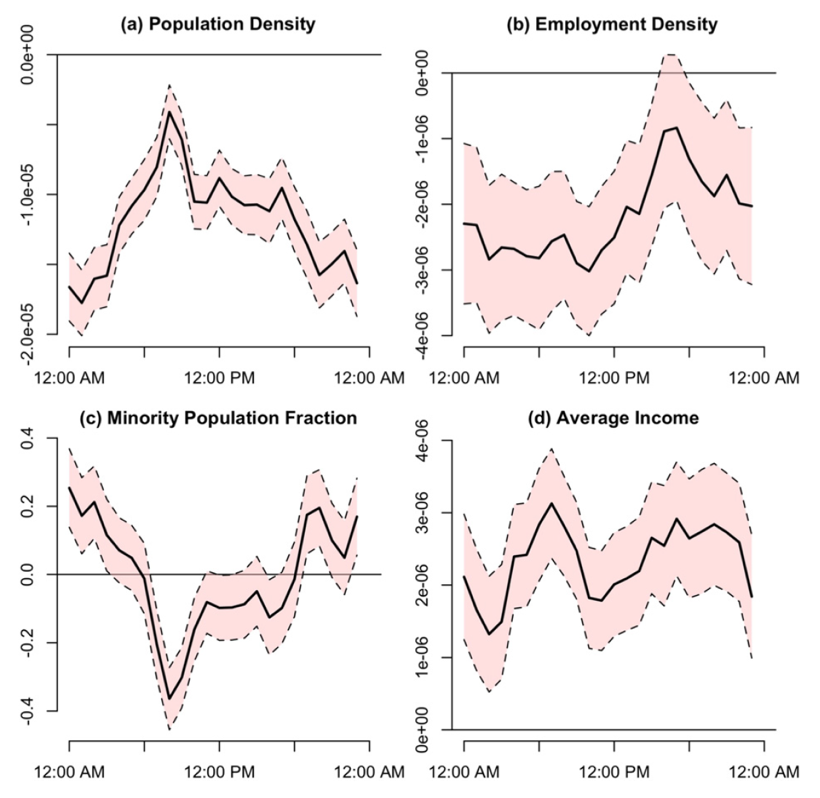
\includegraphics[width=0.6\linewidth]{hughes1.png}
%  \caption{Coefficient estimates and 95\% confidence interval of spatial error model for (a) population density, (b) employment density, (c)minority population fraction, and (d) average income \cite{hughes2016transportation}.}
%  \label{fig:hughes1}
%\end{figure*}
\begin{figure}[!tbp]
  \centering
  \begin{minipage}[b]{0.45\textwidth}
    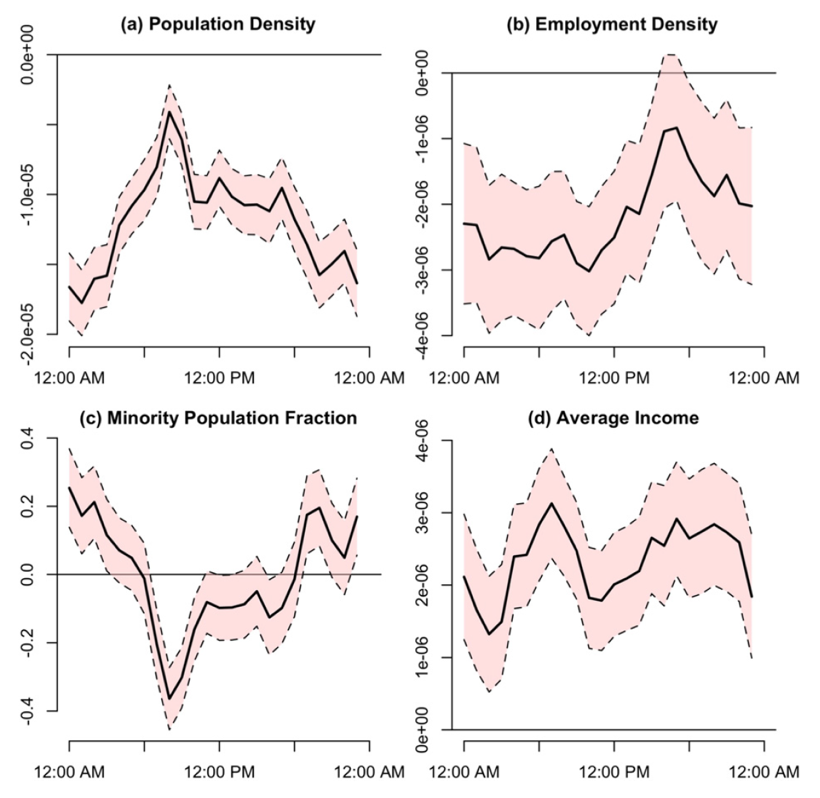
\includegraphics[width=\textwidth]{hughes1.png}
    \caption{Coefficient estimates and 95\% confidence interval of spatial error model for (a) population density, (b) employment density, (c)minority population fraction, and (d) average income \cite{hughes2016transportation}.}
    \label{fig:hughes1}
  \end{minipage}
  \hfill
  \begin{minipage}[b]{0.45\textwidth}
    \centering
    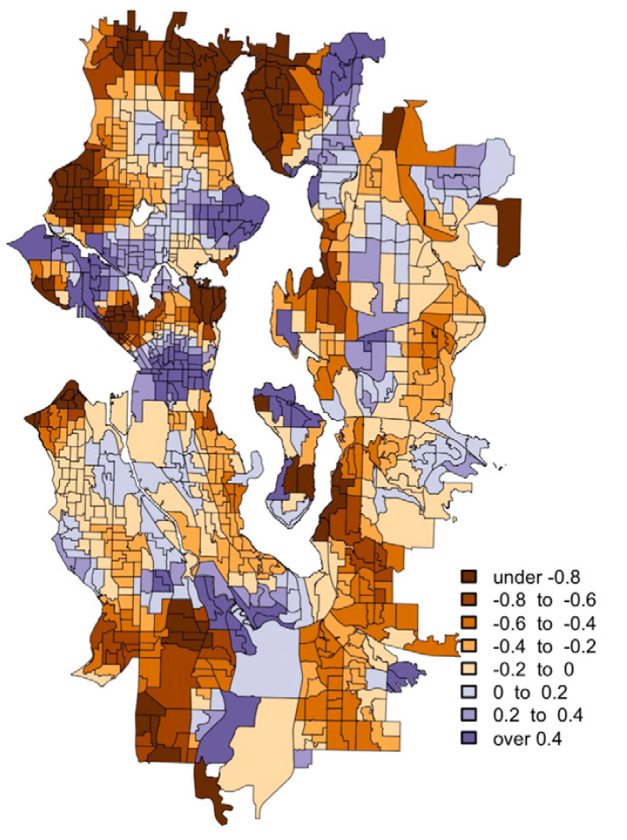
\includegraphics[height=2.9in]{hughes2.png}
    \caption{Coefficients for minority fraction from geographically weighted regression. Purple indicates a positive association between expected waiting time and minority fraction; gold indicates a negative association \cite{hughes2016transportation}.}
    \label{fig:hughes2}
  \end{minipage}
\end{figure}
% across the 24 models representing each hour of the day
Hughes and MacKenzie \cite{hughes2016transportation} investigated the relationships between wait times for UberX and socioeconomic indicators at census block group (CBG) level in Greater Seattle area. They obtained wait times by making UberX requests through Uber API using quasi-randomly selected locations throughout Greater Seattle. They collected about 1 million data points over a two-month period in 2015. Socioeconomic data including population density, employment density, average income, and minority population fraction was collected from the American Community Survey 5-year estimates (ACS). 

They first fitted a regression model with mean waiting times in a CBG as dependent variable and socioeconomic attributes as independent variables. Using a Moran index test, they found significant spatial dependencies among waiting times in different CBG. Subsequently, they developed a spatial error model for each hour of the day to incorporate spatial effect into regression. Results showed that after adjusting the other covariates, higher population density and employment density were associated with shorter waiting time, but that the fraction of minorities in a block group did not significantly associated with waiting times, and that the relationship between these two variables varied between positive and negative throughout the day (Figure \ref{fig:hughes1}). In addition, higher average income is associated with longer wait times, suggesting that low-income areas enjoy better services. 
Geographically weighted regression (GWR) \cite{fotheringham2003geographically} was used to inform different impacts of each socioeconomic variable on different regions. GWR results showed that the relationship between the fraction of minority and wait times is mostly negative. They concluded that ``white and wealthy'' areas do not necessarily enjoy a better TNC service in terms of wait times.

%\begin{figure*}[h]
%  \centering
%  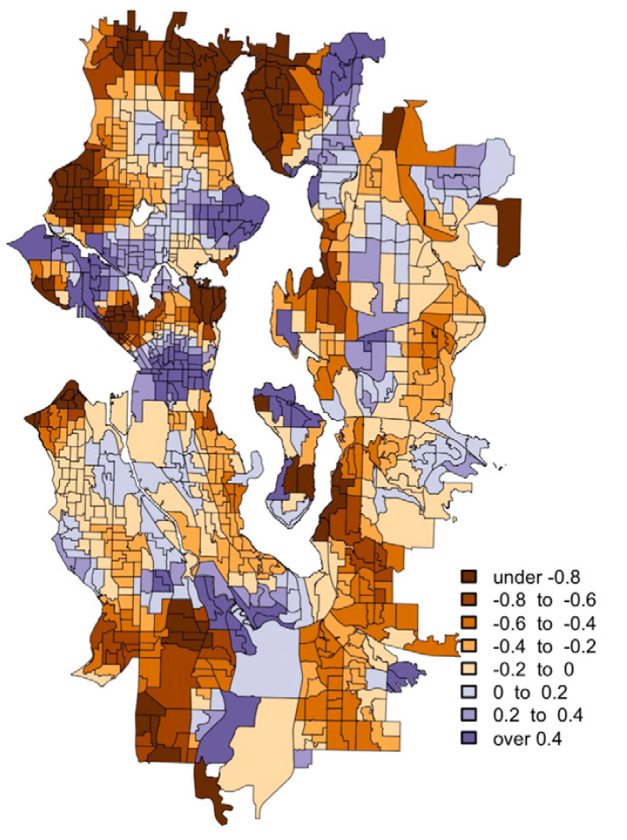
\includegraphics[width=0.35\linewidth]{hughes2.png}
%  \caption{Coefficients for minority fraction from geographically weighted regression. Purple indicates a positive association between expected waiting time and minority fraction; gold indicates a negative association \cite{hughes2016transportation}.}
%  \label{fig:hughes2}
%\end{figure*}

The strength of this study is that it examined both spatial and temporal variations of the effects of different variables (e.g., minority fraction) on TNC waiting times. An interesting addition to this study is to include factors describing the urban form, such as road network into analysis into analysis. For example, the authors found out that higher income is associated with longer waiting time. It is possible that areas with dense road networks tend to experience shorter waiting times, and high-income individuals tend to live in areas with sparse road networks. If this is case, it implies that current urban infrastructure may contribute to the inequalities of new mobility services. For the same reason, it is unclear if the relationships found in this study will generalize to other cities, of which urban forms (e.g., road network, crime rate, employment density, etc.) differ from Seattle. 

Example 1 and Example 2 both examined the equity of service provision in terms of a single indicator (service area coverage and waiting times). These two examples sought to evaluate \textit{equity of opportunity}. While waiting times and docking station locations are important, they do not fully imply the disparities in actual use. For example, individuals without a smartphone cannot use shared bikes even if the docking station is located close to them. The following example approaches this problem from another perspective, namely, focusing on evaluating the \textit{equity of outcome}.  

\paragraph{Example 3: Inequalities in usage of a public bicycle sharing}
Ogilvie and Goodman \cite{ogilvie2012inequalities} explored the correlation between the usage of a bikeshare system in London and socioeconomic attributes. The dataset they use is the anonymized user registration data of a bikeshare system. They examined two dependent variables separately: mean number of trips made by a registered user per month (continuous) and whether a registered user has ever made any trip (binary). They constructed a series of independent variables from the registration data, including gender, place of residence, income deprivation (English Indices of Deprivation) at the level of the Lower Super Output Area (LSOA, a base unit of UK census data), non-White percentage of residential LSOA, distance from residence to nearest bike station, number of stations within 250m of residence, month of registration, etc. 

% percentage of LSOA population commuting by cycling,
The authors employed linear regression to examine the relationship between “mean number of trips per month” and independent variables, and logistic regression to examine the relationship between “ever made any trip” and independent variables. Spatial autocorrelation was accounted for using maximum likelihood estimation. Regression results showed that female users made fewer trips than males per month and users in more deprived areas are less likely to live close to a bike station. After adjusting for the distance from residential area to station, those in more deprived areas made more trips than those in the least deprived areas. They concluded that disparities exist in usage of the system across population, and the system has potentials to fulfill unmet meet if services expand to more deprived areas. 

This study examined the equity of individual-level bikeshare usage. Although the authors found that female users tend to have fewer trips than male users, they cannot determine the cause of this observed relationship. It could be that females tend to have fewer bike trips at night or to regions with high crime rates due to safety concerns. After adjusting for crime rate or time of day, the association between bike usage and gender may change. This brings up another limitation of this research resulted from the use of automatically collected data from bikeshare system. The authors did not have control over the data collection process, so what they could study is also limited. Moreover, constrained by the data availability, the authors had to use area-level socioeconomic variables derived from the postcode of registration debit or credit card. It is thus unclear whether the conclusions would still hold if individual-level variables were available. The temporal scale of the data (7 months) limits the possibility to explore seasonal effects of bike usage. 

% It could be that the authors did not have access to information on when the trips were performed, so the further analysis based on time of day was not possible. 

%This study exposes the tension between privacy and transparency of new mobility data. Equity studies benefit  from individual-level user data, nevertheless, privacy concerns restrict the sharing of such data to the general public. Research is needed to create high quality and privacy-preserving datasets for and beyond transportation equity studies. 


\paragraph{Advantages and limitations of correlational research for equity studies}
By using correlational research, researchers can examine the relationships between transportation provision (or usage) and a wide range of variables collected from various sources. This is especially true when large amount of automatically collected data (e.g., smart card data, bikeshare trip database) is available.  Correlational research is appropriate when researchers are unable to manipulate the variables due to practical or ethical reasons. For example, in equity studies, area-level variables such as average income of a CBG is not controllable. 

One limitation of correlational research is that a significant correlation does not allow the researcher to determine a causal relationship, because there could be many factors that the researcher did not study but contribute to the correlation. And these factors could be independent of mobility service provision. Further inquiry is needed to corroborate the findings from a correlational study. Another limitation is that correlational research heavily depends on data availability and data quality, as discussed in Example 3. 
\subsection{Experimental Research}
Experimental research enables researchers to identify causal relationship. In an experiment design, the researcher seeks to fully control the environment conditions so that variables of interest can be manipulated, while other variables are controlled (or randomized) across conditions. In this way, the effects of variables of interest can be tested by comparing between two or more conditions. Unlike correlational research, experimental research strictly controls for the impacts of variables not of interest, thus allowing the effects of variables of interest to be measured upon the outcome \cite{lazar2017research}. 

\paragraph{Example: Racial and gender discrimination in transportation network companies}
Ge et al.\cite{ge2016racial} studied the racial and gender discrimination in Transportation Network Companies (TNCs). They undertook two randomized control trails, hailing about 1500 rides in Seattle and Boston and recording service quality indicators. In the  Seattle experiment, the treatment is race. Eight RAs (two African American females, two white females, two African American males, and two white males) were hired to request rides. Measures including estimated waiting times, acceptance time (time between trip request and acceptance), actual waiting times (time between acceptance and arrival), trip cancellation rate, trip duration, costs, and ratings were recorded by screenshots for each trip. To control for variables not of interest, the authors adopted a number of strategies. The RAs are undergraduate students, avoiding confounding factors such as age. They were given the identical smartphones using the same carriers, and received the same data collection instructions. The RAs were instructed to minimize their interactions with the driver, preventing the introduction of factors that influence ratings and travel time. Specific routes were developed to control for pick-up locations and travel duration. These routes were randomly assigned to RAs. RAs were also instructed to travel after evening rush hours from Mondays to Thursdays. Ordinary least squares regression (OLS) results showed that acceptance time is longer for African American riders than white riders for both UberX and Lyft. 

In the Boston experiment, the authors adopted a within-group design. They hired eight RAs with a range of ethnic backgrounds summoning UberX or Lyft rides in Boston, each requesting rides under a “white-sounding” name and a “distinctively black name”. This change in design aims to control the differences in data collection practices among RAs. In this case, the treatment is whether the rider has a black sounding name. Other aspects of experiment design are similar to those of the Seattle experiment. OLS results showed that riders with African American-sounding names experienced more frequent trip cancellations, and that African American males have higher cancellation rates than white males. Further analysis revealed that trip cancellations concentrated in pickup locations with low population density. They concluded that racial discrimination exists in TNC services in Seattle and Boston.


\paragraph{Advantages and limitations of experimental research for equity studies}
Experimental research allows for drawing causal conclusions. This is because experiments are conducted in controlled conditions and researchers can claim that the changes in outcomes are caused by the variable of interest. 

Experimental research has notable limitations. First, the requirement that controlling all variables that might influence the outcomes is sometimes not realistic. This is especially true for experiments conducted in a natural environment. For example, in Ge et al.’s Seattle experiment \cite{ge2016racial}, there are variances in the data collection practices (e.g., the time lag between taking screenshots and sending requests) among RAs. This influences the measurement of outcome variables. Second, compared to automatically collected data or survey data, experiments are often not able to produce large amount of data. Data collection in experiments is often expensive and labor-intensive. Finally, although experimental research can determine causal effects (e.g., racial discrimination exists in TNC services in Seattle), it cannot unveil the reasons why the outcome occurred (e.g., why TNC drivers discriminate against certain races). Further investigation through other research methods (e.g., interviews) is needed to understand the phenomenon.  
\begin{figure}[!tbp]
  \centering
  \begin{minipage}[b]{0.48\textwidth}
    \centering
    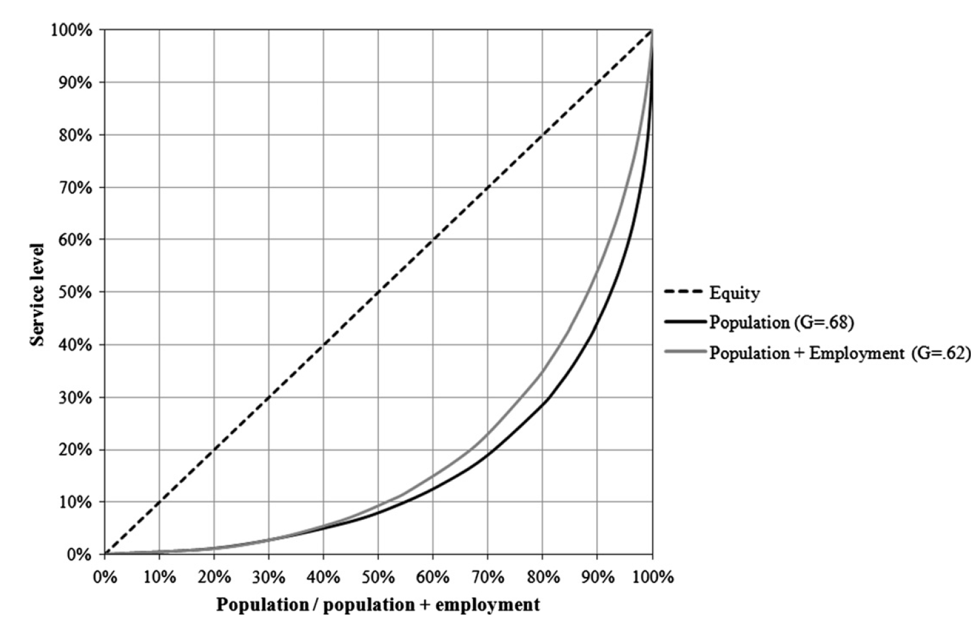
\includegraphics[width=\textwidth]{gini2.png}
    \caption{Use Lorenz curves to compare the equity of public transport service level to demand (population and employment) \cite{delbosc2011using}.}
    \label{fig:gini2}
  \end{minipage}
  \hspace{2cm}
  \begin{minipage}[b]{0.34\textwidth}
    \centering
    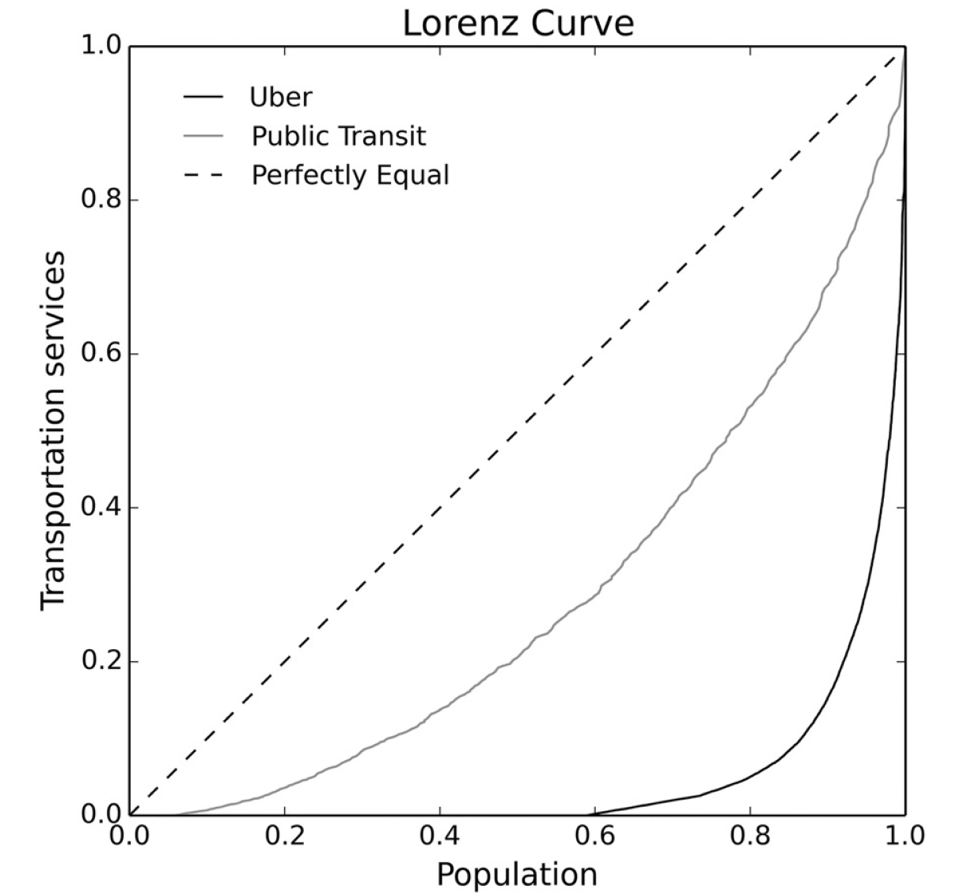
\includegraphics[width=\textwidth]{gini3.png}
    \caption{Use Lorenz curves to compare the equity of public transport and Uber  service level to population \cite{jin2019uber}.}
    \label{fig:gini3}
  \end{minipage}
\end{figure}
\subsection{Equity Metrics}
Metrics that measure the distribution of some mobility system impacts (e.g., service level) have been widely adopted in transportation equity evaluation. Unlike statistical tests which focus on the discovery of discrimination or inequalities, metrics directly gauge the degree of equity by a single value. Equity metrics used in transportation equity research differ but overlap with those used in fairness in machine learning research. The similarities between them partially arise from the fact that both fields borrowed ideas from other domains such as social welfare and economics. For example, Gini coefficient (or Gini index), initially proposed to represent cumulative income and wealth distribution across a population, is one of the most popular equity metrics used in transportation to gauge the equity of transportation resource allocation \cite{ricciardi2015exploring}.  However, Gini index has not yet received much attention in machine learning community \cite{speicher2018unified}. Perhaps this is because fairness in machine learning research has primarily concentrated on classification problems that used in credit scoring, profiling of potential suspects, hiring, etc., for which other metrics are more appropriate. On the other hand, there are a few metrics, such as the “80\% Rule” \cite{useeoc}, were used in both communities \cite{feldman2015certifying}. The following examples introduce the use of Gini index and the "80\% Rule” in transportation equity. 

\paragraph{Example 1: Using Lorenz curves to assess public transport equity in Melbourne}
Delbosc and Currie \cite{delbosc2011using} proposed to use Gini index as an equity metric of public transit service provision. A Lorenz curve is a graphical representation of Gini index. The figure below (see Figure \ref{fig:gini2}) illustrates an example of a Lorenz curve representing the cumulative income across a population. The perfect equitable income distribution is plotted as the dashed line (line of equity) and an inequitable distribution of income is represented by the solid curve (Lorenz curve). A point on the solid curve can be interpreted as X percent (e.g., 70\%) of population shares about Y percent (e.g., 25\%) of the total income of the population. Gini index is the ratio of the area between the line of equity and the Lorenz curve (A), divided by the total area under the line of equity (A+B). 
%A Gini index of zero signifies perfect equity, whereas Gini index of one expresses the maximum inequality. 



%\begin{figure*}[h]
%  \centering
%  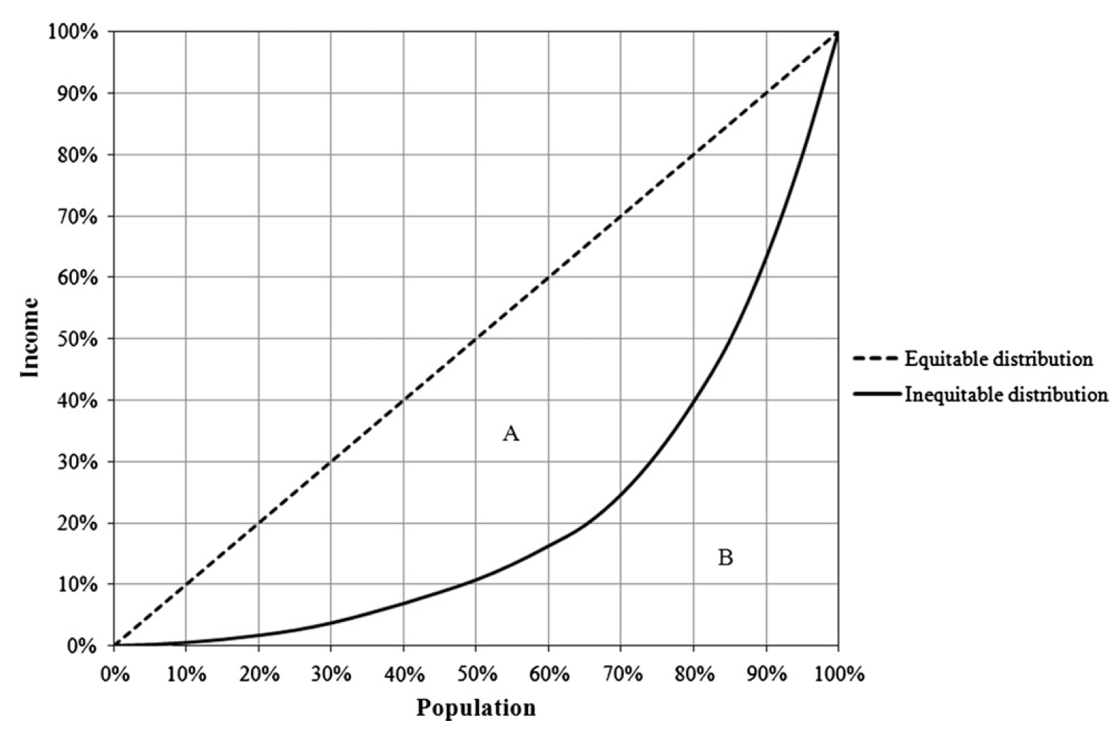
\includegraphics[width=0.6\linewidth]{gini1.png}
%  \caption{Gini coefficient is equal to the area between line of equity and the Lorenz curve (A), divided by the total area under the line of equity (A+B) \cite{delbosc2011using}.}
%  \label{fig:gini1}
%\end{figure*}

Delbosc and Currie applied a gini index to compare the equity of public transport service level to a proxy of demand (population and employment) in Melbourne. Service level of a census tract is expressed as a composite index taking into account bus, tram, and rail service areas and frequency. Using the service level index and the population of each census tract, the authors generated the first Lorenz curve (black solid curve) as shown in Figure \ref{fig:gini2}. The Gini index is 0.68 for overall population in Melbourne. This can be interpreted as 70\% of the population shares 19\% of the public transport services. A second Lorenz curve (a grey solid curve) was calculated, taking into account the employment density. The Gini index for total population and employment is 0.62, appearing more equitable than the first curve. Nevertheless, these two curves suggest that inequalities exist in public transit, with only a small portion of the population enjoying the majority of transit services. 

%\begin{figure*}[h]
  %\centering
  %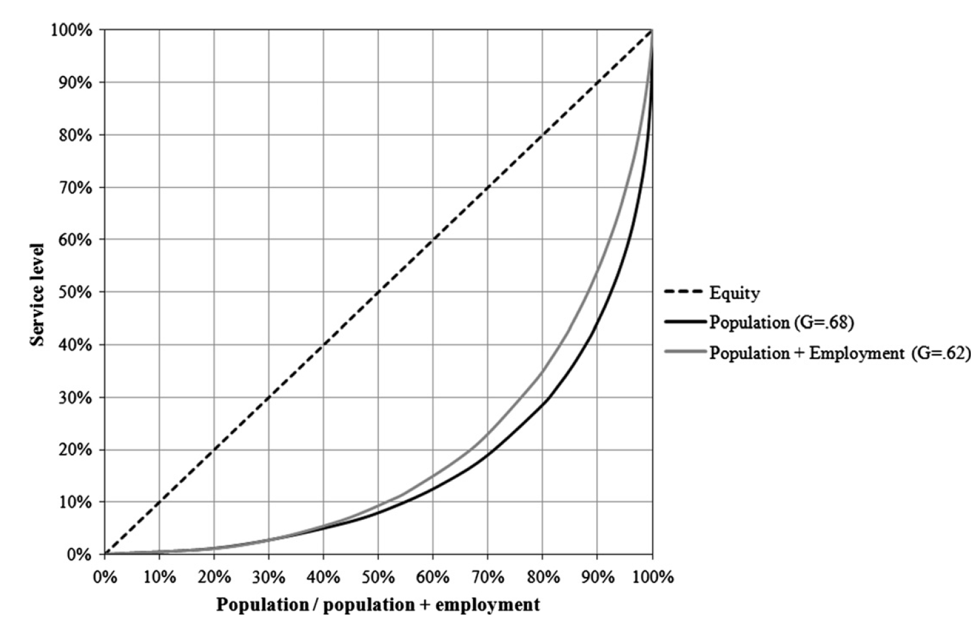
\includegraphics[width=0.6\linewidth]{gini2.png}
  %\caption{Use Lorenz curves to compare the equity of public transport service level to demand (population and employment) \cite{delbosc2011using}.}
%  \label{fig:gini2}
%\end{figure*}



In this example, the Gini index serves as a measure of horizontal equity, that is,  providing equal resources to those equal in need. The need for transportation supply of each census tract is approximated by population and employment density. So the perfect equitable distribution is that every unit of population and jobs shares the same transport resources. The need of special demographic groups (vertical equity) is not considered. 

\paragraph{Example 2: Using Lorenz curves to access the equity of Uber and public transit in New York City}
%\begin{figure*}[h]
%  \centering
%  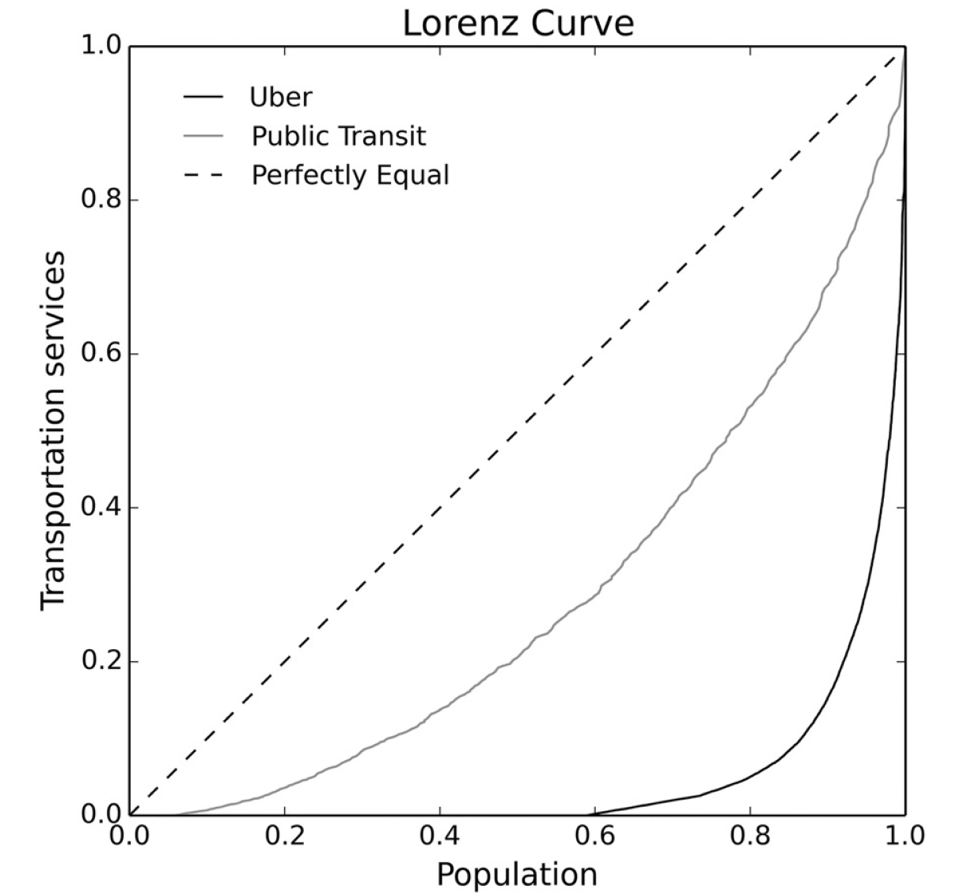
\includegraphics[width=0.4\linewidth]{gini3.png}
%  \caption{Use Lorenz curves to compare the equity of public transport and Uber  service level to population \cite{jin2019uber}.}
%  \label{fig:gini3}
%\end{figure*}
Most recently, Jin et al. \cite{jin2019uber} employed Lorenz curves and Gini index to study the equity of Uber services in New York City (see Figure \ref{fig:gini3}).  They calculated service level for Uber and public transit using a similar approach as Delbosc and Currie \cite{delbosc2011using}. Their results suggested that Uber is less equitable than public transit: 20\% of population shares the 95\% of Uber services. 

They further compared Gini indexes of different boroughs for public transit and public transit + Uber (see Table \ref{fig:gini4}). The results (see Table \ref{fig:gini4}) shows that with Uber, the Gini index of the whole city reduced by about 0.03 on weekdays and by about 0.008 on weekends. This implies that Uber has insignificant impact on the transportation equity of New York City. 


\begin{figure*}[tb]
  \centering
  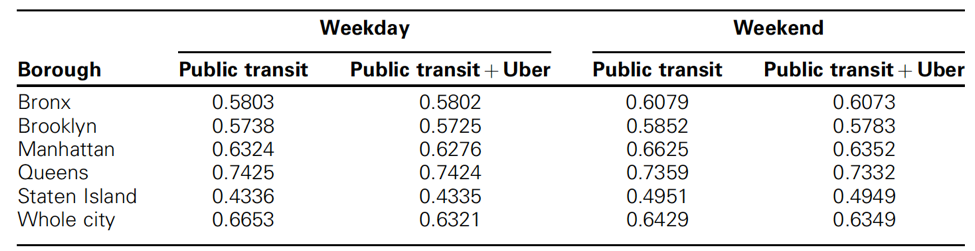
\includegraphics[width=0.8\linewidth]{gini4.png}
  \captionof{table}{Gini coefficient without and with Uber \cite{jin2019uber} }
%   \caption{Gini coefficient without and with Uber \cite{jin2019uber}.}
  \label{fig:gini4}
\end{figure*}

This study exemplifies how Gini index can be used to compare transportation equity across regions and across modes. This is possible because Gini index has several desirable features:  it does not depend on the size of the population, the overall transit supply level, or the geographic units. For example, Gini index can be used to examine the equity of a neighborhood, a city, or a country. And it enables the comparison of equity between a city with high level of transit supply and one with low supply. 

One limitation of Gini index is its heavy reliance on data. As Jin et al. noted, the main reason to choose New York City as study area is data availability. Beyond availability, all data sources have limitations (e.g., census data is not up-to-date) that would be calculated into Gini index. Another limitation lies in the way the service level is calculated. Studies that employed Gini indexes tend to use different methods to calculate service level \cite{feng2014trade}. It is unclear whether changing the service level indicator will significantly affect Gini index. These two limitations suggest that Gini indexes should be interpreted with caution. 

\paragraph{Example 3: Evaluation of the equity of bikeshare system accessibility}
Meng \cite{meng2018evaluation} applied the “80\% Rule” to evaluate access equity of a bikeshare system in Chicago. The “80\% Rule” was advocated by the US Equal Employment Opportunity Commission to detect disparate impacts in employee selection procedures. The 80\% Rule states that if the selection rate for minorities is less than 80\% of the rate of non-minorities, the procedure is deemed to be discriminatory \cite{useeoc}. Similar to Ursaki and Aultman-Hall (see Example 1 of Section \ref{sec:correlation}), the analysis is based on the locations of docking stations. The author created a 0.25-mile buffer around each station as service area, and calculated the demographic characteristics (i.e., race, gender, education, language proficiency, and income level) of population inside each service area. For each station, the equity metric based on the 80\% Rule is calculated as follows:


\begin{equation}
    Ratio = \frac{Number \  of \  minorities / Total \ number \ of \ minorities}{Number \ of \ non-minorities / Total \ number \ of \ non-minorities}
\end{equation}

The results show that more than 33\% of the stations have ratios below 0.8 for all demographic characteristics (except for gender) under examination.

There are several limitations of this study. First, instead of providing a city-level ratio, the authors computed station-level ratios and examined equity using the percentage of stations that violate the 80\% Rule. This approach is problematic when the stations are not equally distributed. It is possible that a majority of the stations are all located in a small portion of the city and they tend to have similar ratios. Second, docking station placement cannot sufficiently represent access to bikeshare, as discussed in Example 1 of Section \ref{sec:correlation}. Despite these weaknesses, this study serves as a typical example of using fairness metrics to evaluate vertical equity in new mobility systems. 

\paragraph{Advantages and limitations of equity metrics}
Equity metric provides a single measure of equity, making it possible to track trends over time and conduct comparative studies between cities. It is easier for non-experts to interpret compared to statistical tests, therefore suited for conveying evaluation results to broader audience.

However, the reliability of metrics heavily depends on the quality of data sources. Moreover, different metrics often reflect competing goals. For example, Gini index measures horizontal equity, emphasizing individuals with equal ability or need gets equal resources. The 80\% Rule shares a similar spirit of group fairness \cite{feldman2015certifying}, which advocates for equal resource distribution across difference demographic groups.  The choice of metrics may significantly affect evaluation results, so the use of multiple metrics is important.   

\subsection{Other methods}
Apart from the three research methods described above, surveys, interviews, and focus groups have been used for transportation equity studies. These methods can be used to develop a deeper understanding of why inequalities exist based on the opinions, attitudes, and experiences from stakeholders of mobility systems. For example, McNeil, Nathan, et al. \cite{mcneil2017breaking} conducted a survey of residents living in underserved neighborhoods with bikesahre stations. The findings revealed that minority respondents have more barriers, for example, costs of membership, to using shared bikes than non-minorities. This helps to explain why providing adequate spatial access to disadvantaged neighborhoods alone is not enough to address the disparities in actual use. 

\section{Transportation Equity and Fairness in Machine learning}

In examining the fairness (equity) definitions from transportation equity community and fair machine learning (FairML) community, I observe that a natural mapping between them can be established, though further effort is needed to create a consistent mapping between concepts in one domain to the other. \textit{Horizontal equity} echoes the spirit of \textit{individual fairness} (similar people should be treated similarly). \textit{Vertical equity} resembles \textit{group fairness} (sensitive attributes should be independent from outcomes). This is true in cities where there is an uneven distribution of transport supply across different socioeconomic groups. Vertical equity encourages compensating for such inequalities by policies favoring disadvantaged groups. This aligns with group fairness that the level of transportation supply in a city should be the same across different groups. Vertical equity and group fairness are only ``roughly'' related because by definition, group fairness stresses ``independence'' between sensitive attributes and outcome, whereas vertical equity does not.   

%\begin{figure*}[h]
%  \centering
%  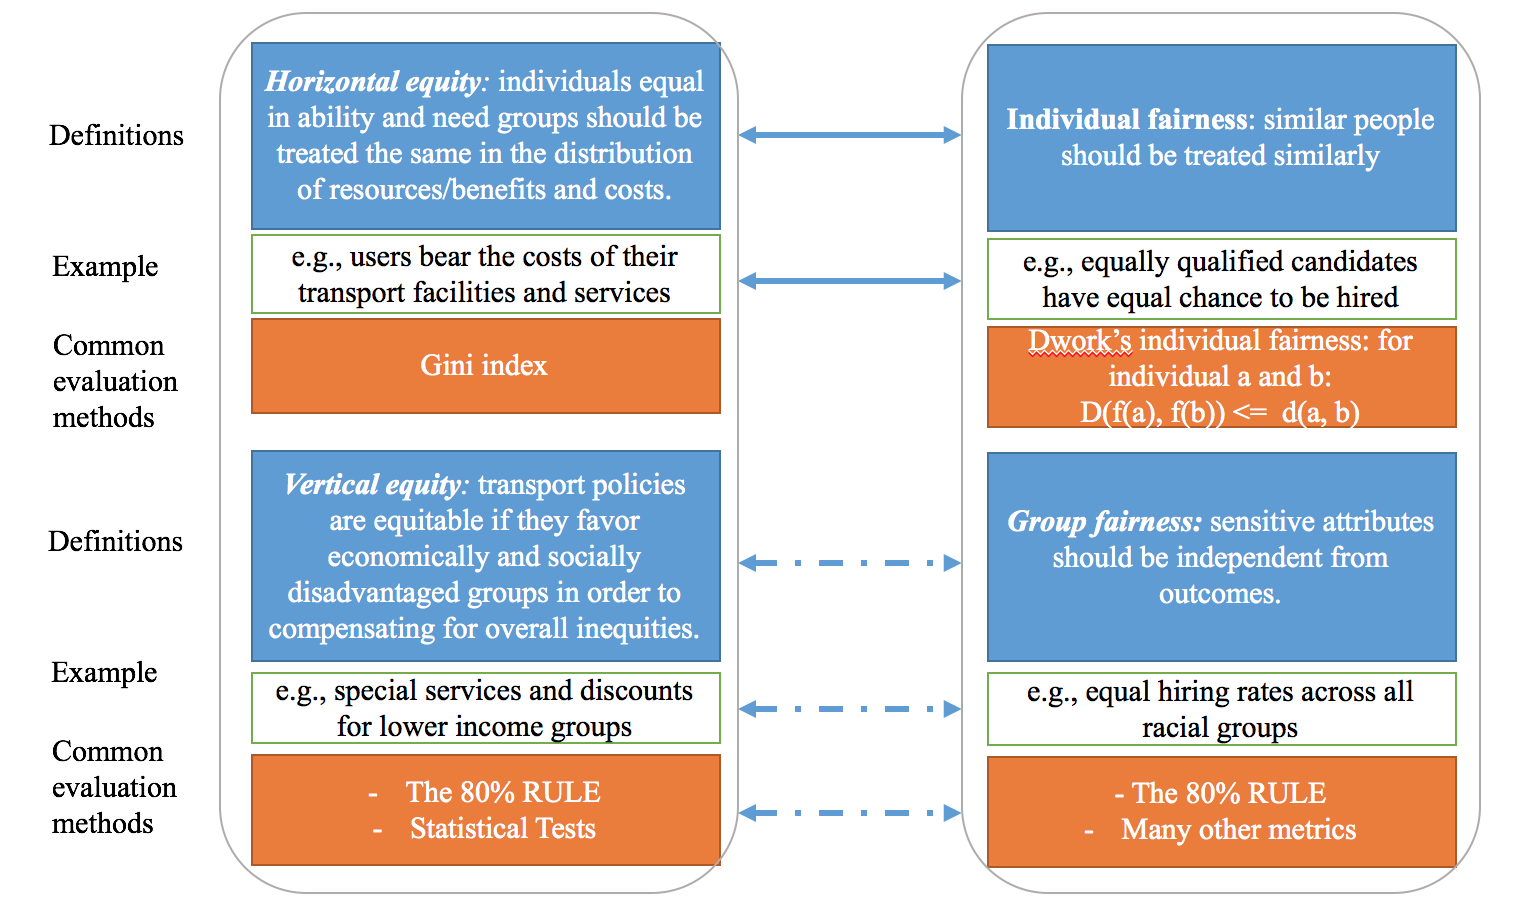
\includegraphics[width=0.8\linewidth]{mapping.png}
%  \caption{Mapping of concepts, examples, and methods between transportation equity (left) and fair machine learning (right)}
%  \label{fig:mapping}
%\end{figure*}

The most commonly used method for evaluating horizontal equity is Gini index. It has not attracted much attention in machine learning community. This may be partially due to the fact that not much attention has been paid to resource allocation problems in fair machine learning research. On the other hand, machine learning community has developed a few metrics for individual fairness. Individual fairness requires that the ``similarity'' between a pair of individuals from two demographic groups respectively has to be defined. For example, in making hiring decisions, the algorithm has to possess perfect knowledge of how to compare the ``qualification'' of two individuals. This is often not realistic in  practice and we have to come up with a suitable similarity metric that is best agreed upon among domain experts of a task. Theoretically, individual fairness can be used to evaluate horizontal equity. For example, in a simplified shared bike allocation problem, we use population and employment density as the demand for bikes. Then the differences in demand between two areas $a$ and $b$ can be expressed as $d(a, b)$ according to some similarity function $d$. Suppose we have an algorithm assigning bikes to areas, the number of bikes that area $a$ and $b$ will get is $f(a)$ and $f(b)$, respectively. A fair allocation satisfying individual fairness requires that for every two pairs of areas in the city: $D(f(a) , f(b)) <= d(a,b)$, where $D$ is another similarity function. The difficulty again, lies in the fact that we do not have perfect knowledge to determine the similarity in demand between two areas. 

The majority of transportation equity research focuses on vertical equity. Likewise, more attention has been devoted to group fairness than individual fairness in machine learning community. Transportation equity heavily employs statistical tests for equity analysis, which is appropriate for discovering unfairness. Machine learning uses fairness metrics much more often, because metrics allow researchers to reduce achieving fairness goals to a much simpler problem: minimizing a value that represents unfairness. This is also valid in terms of algorithm design. In fact, some metrics, such as the 80\% Rule, have been used in both communities. This connection may open great possibilities for bridging these two domains.   

Fair machine learning community focuses almost exclusively on methods, whereas transportation equity concerns more about applications, policies, and interventions. Although fair machine learning approaches hold great promises in optimizing resource allocation in mobility settings, there is a long way to go to design, deploy, and evaluate a fairness-aware data-driven system as a real-world application. At the end of this paper, I hope to highlight the urgency of convergence of these two fields. Ultimately, researchers with knowledge in both fields, practitioners, policy-makers, and citizens should work together towards a common goal: a fair and effective transportation system for  all citizens. 


\section{Conclusion}
% \looseness-1
This paper summarized the findings and methods of equity studies in mobility systems, with a focus on new mobility systems. For new mobility services, it is generally agreed that disparities exist in the access and use of docked bikeshare system, but the equity implications of ride-hailing are still unclear. Further research is needed to understand how to deliver a more equitable new mobility system to serve the need of different groups. Many research methods have been employed in transportation equity studies. Different methods vary in their objectives, strengths and weaknesses. Correlational research can exploit a wide range of data sources and discover associations among many factors, but it cannot determine causal relationships. Equity metrics enable comparative studies among cities and assessment of changes over time, but their reliability is highly dependent on data. Experimental research can produce reliable findings, but is expensive and difficult to control all extraneous variables. The choice of research methods depends on research goals, and multiple methods can be used together to complement each other. 

Given the similarities in objectives, concepts, and methods between transportation equity community and fairness in machine learning community, bridging these two domains together holds promise to enable multi-disciplinary breakthroughs. 


\begin{thebibliography}{10}
\itemsep=1pt
\begin{small}

\bibitem{AbiteboulHVBook}
Serge Abiteboul, Richard Hull, and Victor Vianu.
\newblock {\em Foundations of Databases}.
\newblock Addison-Wesley, 1995.

\bibitem{ainy2015approximated}
Eleanor Ainy, Pierre Bourhis, Susan~B Davidson, Daniel Deutch, and Tova Milo.
\newblock Approximated summarization of data provenance.
\newblock In {\em Proceedings of the 24th ACM International on Conference on
  Information and Knowledge Management}, pages 483--492. ACM, 2015.

\bibitem{antenucci2018constraint}
Dolan Antenucci and Michael Cafarella.
\newblock Constraint-based explanation and repair of filter-based
  transformations.
\newblock {\em Proceedings of the VLDB Endowment}, 11(9):947--960, 2018.

\bibitem{avin2005identifiability}
Chen Avin, Ilya Shpitser, and Judea Pearl.
\newblock Identifiability of path-specific effects.
\newblock In {\em Proceedings of International Joint Conference on Artificial
  Intelligence}, pages 357--363, 2005.

\bibitem{bertossi2017causes}
Leopoldo Bertossi and Babak Salimi.
\newblock Causes for query answers from databases: Datalog abduction,
  view-updates, and integrity constraints.
\newblock {\em International Journal of Approximate Reasoning}, 90:226--252,
  2017.

\bibitem{DBLP:series/synthesis/2011Bertossi}
Leopoldo~E. Bertossi.
\newblock {\em Database Repairing and Consistent Query Answering}.
\newblock Synthesis Lectures on Data Management. Morgan {\&} Claypool
  Publishers, 2011.

\bibitem{calders2009building}
Toon Calders, Faisal Kamiran, and Mykola Pechenizkiy.
\newblock Building classifiers with independency constraints.
\newblock In {\em Data mining workshops, 2009. ICDMW'09. IEEE international
  conference on}, pages 13--18. IEEE, 2009.

\bibitem{chapman2009not}
Adriane Chapman and HV~Jagadish.
\newblock Why not?
\newblock In {\em Proceedings of the 2009 ACM SIGMOD International Conference
  on Management of data}, pages 523--534. ACM, 2009.

\bibitem{chouldechova2017fair}
Alexandra Chouldechova.
\newblock Fair prediction with disparate impact: A study of bias in recidivism
  prediction instruments.
\newblock {\em Big data}, 5(2):153--163, 2017.

\bibitem{corbett2017algorithmic}
Sam Corbett-Davies, Emma Pierson, Avi Feller, Sharad Goel, and Aziz Huq.
\newblock Algorithmic decision making and the cost of fairness.
\newblock In {\em Proceedings of the 23rd ACM SIGKDD International Conference
  on Knowledge Discovery and Data Mining}, pages 797--806. ACM, 2017.

\bibitem{courtland2018bias}
Rachel Courtland.
\newblock Bias detectives: the researchers striving to make algorithms fair.
\newblock {\em Nature}, 558, 2018.

\bibitem{dwork2012fairness}
Cynthia Dwork, Moritz Hardt, Toniann Pitassi, Omer Reingold, and Richard Zemel.
\newblock Fairness through awareness.
\newblock In {\em Proceedings of the 3rd innovations in theoretical computer
  science conference}, pages 214--226. ACM, 2012.

\bibitem{galhotra2017fairness}
Sainyam Galhotra, Yuriy Brun, and Alexandra Meliou.
\newblock Fairness testing: testing software for discrimination.
\newblock In {\em Proceedings of the 2017 11th Joint Meeting on Foundations of
  Software Engineering}, pages 498--510. ACM, 2017.

\bibitem{glavic2007data}
Boris Glavic and Klaus Dittrich.
\newblock Data provenance: A categorization of existing approaches.
\newblock {\em Datenbanksysteme in Business, Technologie und Web (BTW
  2007)--12. Fachtagung des GI-Fachbereichs" Datenbanken und
  Informationssysteme"(DBIS)}, 2007.

\bibitem{hardt2016equality}
Moritz Hardt, Eric Price, Nati Srebro, et~al.
\newblock Equality of opportunity in supervised learning.
\newblock In {\em Advances in neural information processing systems}, pages
  3315--3323, 2016.

\bibitem{kilbertus2017avoiding}
Niki Kilbertus, Mateo~Rojas Carulla, Giambattista Parascandolo, Moritz Hardt,
  Dominik Janzing, and Bernhard Sch{\"o}lkopf.
\newblock Avoiding discrimination through causal reasoning.
\newblock In {\em Advances in Neural Information Processing Systems}, pages
  656--666, 2017.

\bibitem{kusner2017counterfactual}
Matt~J Kusner, Joshua Loftus, Chris Russell, and Ricardo Silva.
\newblock Counterfactual fairness.
\newblock In {\em Advances in Neural Information Processing Systems}, pages
  4069--4079, 2017.

\bibitem{larson2016we}
Jeff Larson, Surya Mattu, Lauren Kirchner, and Julia Angwin.
\newblock How we analyzed the compas recidivism algorithm.
\newblock {\em ProPublica (5 2016)}, 9, 2016.

\bibitem{DBLP:conf/pods/LevyMSS95}
Alon~Y. Levy, Alberto~O. Mendelzon, Yehoshua Sagiv, and Divesh Srivastava.
\newblock Answering queries using views.
\newblock In {\em Proceedings of the Fourteenth {ACM} {SIGACT-SIGMOD-SIGART}
  Symposium on Principles of Database Systems, May 22-25, 1995, San Jose,
  California, {USA}}, pages 95--104, 1995.

\bibitem{adult}
M.~Lichman.
\newblock Uci machine learning repository, 2013.

\bibitem{DBLP:conf/pods/LivshitsKR18}
Ester Livshits, Benny Kimelfeld, and Sudeepa Roy.
\newblock Computing optimal repairs for functional dependencies.
\newblock In {\em Proceedings of the 37th {ACM} {SIGMOD-SIGACT-SIGAI} Symposium
  on Principles of Database Systems, Houston, TX, USA, June 10-15, 2018}, pages
  225--237, 2018.

\bibitem{loftus2018causal}
Joshua~R Loftus, Chris Russell, Matt~J Kusner, and Ricardo Silva.
\newblock Causal reasoning for algorithmic fairness.
\newblock {\em CoRR}, abs/1805.05859, 2018.

\bibitem{meliou2010complexity}
Alexandra Meliou, Wolfgang Gatterbauer, Katherine~F Moore, and Dan Suciu.
\newblock The complexity of causality and responsibility for query answers and
  non-answers.
\newblock {\em Proceedings of the VLDB Endowment}, 4(1):34--45, 2010.

\bibitem{mintz2009distant}
Mike Mintz, Steven Bills, Rion Snow, and Dan Jurafsky.
\newblock Distant supervision for relation extraction without labeled data.
\newblock In {\em Proceedings of the Joint Conference of the 47th Annual
  Meeting of the ACL and the 4th International Joint Conference on Natural
  Language Processing of the AFNLP: Volume 2-Volume 2}, pages 1003--1011.
  Association for Computational Linguistics, 2009.

\bibitem{nabi2018fair}
Razieh Nabi and Ilya Shpitser.
\newblock Fair inference on outcomes.
\newblock In {\em Proceedings of the... AAAI Conference on Artificial
  Intelligence. AAAI Conference on Artificial Intelligence}, volume 2018, page
  1931. NIH Public Access, 2018.

\bibitem{pearl2003causality}
Judea Pearl.
\newblock Causality: models, reasoning, and inference.
\newblock {\em Econometric Theory}, 19(675-685):46, 2003.

\bibitem{pearl2009causality}
Judea Pearl.
\newblock {\em Causality}.
\newblock Cambridge university press, 2009.

\bibitem{pearl2009causal}
Judea Pearl et~al.
\newblock Causal inference in statistics: An overview.
\newblock {\em Statistics Surveys}, 3:96--146, 2009.

\bibitem{DBLP:conf/sigmod/PopaDST00}
Lucian Popa, Alin Deutsch, Arnaud Sahuguet, and Val Tannen.
\newblock A chase too far?
\newblock In {\em Proceedings of the 2000 {ACM} {SIGMOD} International
  Conference on Management of Data, May 16-18, 2000, Dallas, Texas, {USA.}},
  pages 273--284, 2000.

\bibitem{ratner2017snorkel}
Alexander Ratner, Stephen~H Bach, Henry Ehrenberg, Jason Fries, Sen Wu, and
  Christopher R{\'e}.
\newblock Snorkel: Rapid training data creation with weak supervision.
\newblock {\em Proceedings of the VLDB Endowment}, 11(3):269--282, 2017.

\bibitem{ratner2016data}
Alexander~J Ratner, Christopher~M De~Sa, Sen Wu, Daniel Selsam, and Christopher
  R{\'e}.
\newblock Data programming: Creating large training sets, quickly.
\newblock In {\em Advances in neural information processing systems}, pages
  3567--3575, 2016.

\bibitem{raykar2010learning}
Vikas~C Raykar, Shipeng Yu, Linda~H Zhao, Gerardo~Hermosillo Valadez, Charles
  Florin, Luca Bogoni, and Linda Moy.
\newblock Learning from crowds.
\newblock {\em Journal of Machine Learning Research}, 11(Apr):1297--1322, 2010.

\bibitem{roy2014formal}
Sudeepa Roy and Dan Suciu.
\newblock A formal approach to finding explanations for database queries.
\newblock In {\em Proceedings of the 2014 ACM SIGMOD international conference
  on Management of data}, pages 1579--1590. ACM, 2014.

\bibitem{rubin1970thesis}
Donald~B Rubin.
\newblock {\em The Use of Matched Sampling and Regression Adjustment in
  Observational Studies}.
\newblock Ph.D. Thesis, Department of Statistics, Harvard University,
  Cambridge, MA, 1970.

\bibitem{rubin1986statistics}
Donald~B Rubin.
\newblock Statistics and causal inference: Comment: Which ifs have causal
  answers.
\newblock {\em Journal of the American Statistical Association},
  81(396):961--962, 1986.

\bibitem{rubin2008comment}
Donald~B Rubin.
\newblock Comment: The design and analysis of gold standard randomized
  experiments.
\newblock {\em Journal of the American Statistical Association},
  103(484):1350--1353, 2008.

\bibitem{russell2017worlds}
Chris Russell, Matt~J Kusner, Joshua Loftus, and Ricardo Silva.
\newblock When worlds collide: integrating different counterfactual assumptions
  in fairness.
\newblock In {\em Advances in Neural Information Processing Systems}, pages
  6414--6423, 2017.

\bibitem{DBLP:conf/icdt/SalimiB15}
Babak Salimi and Leopoldo~E. Bertossi.
\newblock From causes for database queries to repairs and model-based diagnosis
  and back.
\newblock In {\em ICDT}, pages 342--362, 2015.

\bibitem{salimi2016quantifying}
Babak Salimi, Leopoldo~E Bertossi, Dan Suciu, and Guy Van~den Broeck.
\newblock Quantifying causal effects on query answering in databases.
\newblock In {\em TaPP}, 2016.

\bibitem{salimi2018hypdb}
Babak Salimi, Corey Cole, Peter Li, Johannes Gehrke, and Dan Suciu.
\newblock Hypdb: a demonstration of detecting, explaining and resolving bias in
  olap queries.
\newblock {\em Proceedings of the VLDB Endowment}, 11(12):2062--2065, 2018.

\bibitem{salimi2018bias}
Babak Salimi, Johannes Gehrke, and Dan Suciu.
\newblock Bias in olap queries: Detection, explanation, and removal.
\newblock In {\em Proceedings of the 2018 International Conference on
  Management of Data}, pages 1021--1035. ACM, 2018.

\bibitem{salimi2019capuchin}
Babak Salimi, Luke Rodriguez, Bill Howe, and Dan Suciu.
\newblock Capuchin: Causal database repair for algorithmic fairness.
\newblock {\em CoRR}, abs/1902.08283, 2019.

\bibitem{salimi2019interventional}
Babak Salimi, Luke Rodriguez, Bill Howe, and Dan Suciu.
\newblock Interventional fairness: Causal database repair for algorithmic
  fairness.
\newblock In {\em Proceedings of the 2019 International Conference on
  Management of Data}, pages 793--810. ACM, 2019.

\bibitem{simoiu2017problem}
Camelia Simoiu, Sam Corbett-Davies, Sharad Goel, et~al.
\newblock The problem of infra-marginality in outcome tests for discrimination.
\newblock {\em The Annals of Applied Statistics}, 11(3):1193--1216, 2017.

\bibitem{verma2018fairness}
Sahil Verma and Julia Rubin.
\newblock Fairness definitions explained.
\newblock In {\em 2018 IEEE/ACM International Workshop on Software Fairness
  (FairWare)}, pages 1--7. IEEE, 2018.

\bibitem{xu2018provenance}
Jane Xu, Waley Zhang, Abdussalam Alawini, and Val Tannen.
\newblock Provenance analysis for missing answers and integrity repairs.
\newblock {\em IEEE Data Eng. Bull.}, 41(1):39--50, 2018.

\bibitem{zafar2017fairness}
Muhammad~Bilal Zafar, Isabel Valera, Manuel Gomez~Rodriguez, and Krishna~P
  Gummadi.
\newblock Fairness beyond disparate treatment \& disparate impact: Learning
  classification without disparate mistreatment.
\newblock In {\em Proceedings of the 26th International Conference on World
  Wide Web}, pages 1171--1180. International World Wide Web Conferences
  Steering Committee, 2017.

\bibitem{zliobaite2015survey2}
Indre Zliobaite.
\newblock A survey on measuring indirect discrimination in machine learning.
\newblock {\em CoRR}, abs/1511.00148, 2015.

		

\end{small}
\end{thebibliography} 	



% \bibliographystyle{unsrt}
% \bibliography{references}  %%% Remove comment to use the external .bib file (using bibtex).
%%% and comment out the ``thebibliography'' section.


%%% Comment out this section when you \bibliography{references} is enabled.
% \begin{thebibliography}{1}

% \bibitem{kour2014real}
% George Kour and Raid Saabne.
% \newblock Real-time segmentation of on-line handwritten arabic script.
% \newblock In {\em Frontiers in Handwriting Recognition (ICFHR), 2014 14th
%   International Conference on}, pages 417--422. IEEE, 2014.

% \bibitem{kour2014fast}
% George Kour and Raid Saabne.
% \newblock Fast classification of handwritten on-line arabic characters.
% \newblock In {\em Soft Computing and Pattern Recognition (SoCPaR), 2014 6th
%   International Conference of}, pages 312--318. IEEE, 2014.

% \bibitem{hadash2018estimate}
% Guy Hadash, Einat Kermany, Boaz Carmeli, Ofer Lavi, George Kour, and Alon
%   Jacovi.
% \newblock Estimate and replace: A novel approach to integrating deep neural
%   networks with existing applications.
% \newblock {\em arXiv preprint arXiv:1804.09028}, 2018.

% \end{thebibliography}


\end{document}

% \end{document}

\end{article}


\begin{article}
{Fairness and Diversity in Public Resource Allocation Problems}
{Nawal Benabbou, Mithun Chakraborty, Yair Zick}
\graphicspath{{submissions/Zick/}}
\documentclass[11pt,dvipdfmx]{article}

\usepackage{deauthor,times}%Compulsory packages

\usepackage{bmpsize}
% \RequirePackage[dvips]{graphicx}


% \graphicspath{{zick/}}

\usepackage{url}
\usepackage{wrapfig,booktabs,multirow}
% \usepackage[ruled,linesnumbered]{algorithm2e}
\usepackage{subcaption}
\usepackage{amsmath}
\usepackage{amsfonts,amssymb}
\usepackage{xspace}
\usepackage{tcolorbox}


\newcommand{\USW}{\mathtt{USW}}
\newcommand{\R}{\mathbb{R}}
\newcommand{\N}{\mathbb{N}}
\newcommand{\OPT}{\mathrm{OPT}}
\newcommand{\ASTC}{\textsc{AssignTC}\xspace}
\newcommand{\PoD}{\mathit{PoD}}
\newcommand{\tup}[1]{\langle #1 \rangle}
\newcommand{\poly}{\mathit{poly}}

\begin{document}

\title{Fairness and Diversity in Public Resource Allocation Problems\footnote{Parts of this article are published in AAMAS 2018 \cite{benabbou2017diversity} and accepted to IJCAI 2019 \cite{benabbou2019fairness}.}}

\author{Nawal Benabbou$^1$, Mithun Chakraborty$^2$, Yair Zick$^2$\\
	$^1$Sorbonne Universit\'e, CNRS, Laboratoire d'Informatique de Paris 6, LIP6 F-75005 Paris, France\\ 
	\texttt{nawal.benabbou@lip6.fr}\\
	$^2$Department of Computer Science, National University of Singapore, Singapore\\
	\texttt{\{mithun,zick\}@comp.nus.edu.sg}
}

\maketitle             

\begin{abstract}
In this article, we address important extensions to the problem of allocating indivisible items to a population of agents: The agents are partitioned into disjoint groups on the basis of attributes (e.g., ethnicity) and we want the overall utility of the allocation to respect some notion of \emph{diversity} and/or \emph{fairness} with respect to these groups. We study two specific incarnations of this general problem. First, we address a constrained optimization problem, inspired by diversity quotas in some real-world allocation problems, where the items are also partitioned into blocks and there is an upper bound on the number of items from each block that can be assigned to agents in each group. We theoretically analyze the price of diversity -- a measure of the overall welfare loss due to these capacity constraints -- and report experiments based on two real-world data sets (Singapore public housing and Chicago public school admissions) comparing this constrained optimization-based approach with a lottery mechanism with similar quotas. Next, instead of imposing hard constraints, we cast the problem as a variant of fair allocation of indivisible goods -- we treat each group of agents as a single entity receiving a bundle of items whose valuation is the maximum total utility of matching agents in that group to items in that bundle; we present algorithms that achieve a standard relaxation of envy-freeness in conjunction with specific efficiency criteria.
%\keywords{Fair Allocation of Indivisible Items  \and Typewise Envy-freeness up to one item \and Non-wasteful Allocation.}
\end{abstract}

\section{Introduction}\label{sec:intro}
Over the years, the Singapore government has adopted several social integration measures, to accommodate its multi-ethnic and multi-cultural population; one of these is the {\em Ethnic Integration Policy} (EIP) used by the Housing and Development Board (HDB) since 1989 \cite{Parl1989} to determine housing allocations. This government body is charged with the construction of government subsidized public housing estates, and selling them to Singapore residents. 
The EIP sets upper bounds on the percentage of flats in every estate that can be owned by households of every major ethnic group: since 5 March 2010, every HDB housing block is required to hold no more than $87\%$ Chinese, $25\%$ Malay, and $15\%$ Indian/Others \cite{HDB10PR,deng2013publichousing}. 
These ethnic quotas prevent the over-representation of any one group in an estate (resulting in de-facto segregation). 
HDB uses a lottery to allocate new developments: all applicants who apply for a particular development pick their flats in a random order. 
Under the lottery mechanism, applicants selected later in the order may not get their top choices; in fact, they may be rejected because the quota for their ethnic group has been filled, {\em even if there are empty flats that they are willing to take}.
\begin{example}
	Consider an estate with 100 flats; Amirah (who is ethnically Malay) receives a queue number of 30 --- i.e., she is the 30th person to choose a flat; if, by random chance, 25 ethnic Malays precede her in the queue and pick before her, the ethnic quota for Malays (25\%) will be filled and Amirah will no longer be allowed to select a flat in that estate. On the other hand, if Amirah is 110th in line but all families preceding her in the queue are ethnically Chinese, then at most 87 out of the 100 flats will be taken (since the Chinese have an 87\% quota) and Amirah will have at least 13 flats to choose from. \hfill $\blacklozenge$
\end{example}
Over $72\%$ of Singapore apartments are HDB flats~\cite{Sing2018}, housing an estimated $81\%$ of Singapore residents \cite{HDB18keystats} as of 2018; thus, the HDB public housing market has a significant impact on the life and welfare -- both individual and collective -- of this island nation \cite{chua1991race,deng2013publichousing,kim2013singapore,sim2003public,wong2014estimating}. 
The HDB lottery mechanism, coupled with ethnicity constraints, adds another layer of complexity to what is, at its core, similar to the classic weighted bipartite matching or \emph{assignment} problem \cite{kuhn1955hungarian,munkres1957algo}: agents (buyer households) have idiosyncratic values/utilities for items (flats) while a central planner (HDB) wishes to allocate at most one item to each agent and vice versa, with the economic criterion of \emph{overall utility/welfare/efficiency} in mind -- but also with an added social goal of \emph{promoting diversity}. 
Inspired by diversity-respecting allocation mechanisms --- prevalent not only in Singapore public housing but also in other domains such as matching residents to hospitals in Japan, school admissions in many U.S. cities, and more \cite{kamada2015efficient,USedu2017,fragiadakis2017improving} --- we formally study the balance between maximizing allocative welfare and promoting allocative diversity. This underlying problem of allocation/assignment of goods distinguishes our contribution from the extensive literature on fairness and diversity in subset selection (see e.g., \cite{stoyanovich2018online,bredereck2018multiwinner} and references therein). 

In Section~\ref{sec:assigntc}, we analyze a (simplified) HDB housing market as an extension to the assignment problem where the sets of agents and items are partitioned into subsets called \emph{types} and \emph{blocks} respectively; there is a pre-specified upper bound on the number of agents of each type that can be assigned items in each block, called \emph{type-block capacities}. 
We analyze the {\em price of diversity}, i.e., the fractional loss in the overall (optimal) welfare due to these capacity constraints, and relate it to a measure of \emph{type disparity}; we also report simulations based on recent, real-world data sets, comparing our constrained optimization approach with a lottery mechanism with ethnicity quotas in terms of welfare.     

In Section~\ref{sec:grfair}, we present an alternative approach towards the efficiency-diversity trade-off, drawing on and adding to the rich literature on the fair division of indivisible goods (see e.g., \cite{procaccia2014fair,caragiannis2016unreasonable,kurokawa2016can,barman2017finding,barman2017approx}). Here, each type is represented by a \emph{super-agent} that is allocated a \emph{bundle} of items; the super-agent's valuation of a bundle is given by the maximum utility assignment of items in the bundle to agents of that type. When agent-item utilities are binary, we provide a polynomial-time algorithm that computes an allocation with the maximum (utilitarian) social welfare while satisfying a popular fairness criterion: \emph{envy-freeness up to one item} (EF1) \cite{budish2011combinatorial}; for arbitrary real-valued utilities, we show experimentally that a heuristic extension of the classic \emph{envy-graph algorithm} due to Lipton et al. \cite{lipton2004approximately} produces an EF1 allocation with low \emph{waste} (a new inefficiency concept that we have introduced for this setting).

\section{Diversity through hard capacity constraints}\label{sec:assigntc}
First, let us rigorously formulate the welfare maximization problem in a bipartite matching setting under type-block capacity constraints. Detailed proofs of all theoretical results in this section can be found in Benabbou et al. \cite{benabbou2017diversity}. Throughout the paper, for $s \in \N$, we denote the set $\{1, 2,\ldots, s\}$ by $[s]$. 
\begin{definition}[\ASTC]\label{def:AwTC}
	An instance of the Assignment with Type Constraints (\ASTC) problem is given by: (i) a set $N$ of $n$ agents partitioned into $k$ types $N_1,\dots, N_k$, (ii) a set $M$ of $m$ items/goods partitioned into $l$ blocks $M_1,\dots,M_l$, (iv) a utility $u(i,j) \in \R_+$ for each agent $i \in N$ and each item $j \in M$, and (iv) a capacity $\lambda_{pq} \in \N$ for all $(p,q) \in [k]  \times [l]$; $\lambda_{pq}$ is an upper bound on the number of agents of type $N_p$ allowed in block $M_q$. W.l.o.g. we assume that for all $p,q$, $\lambda_{pq} \le |M_q|$.
\end{definition}
An assignment of items to agents, which we will also sometimes call an $(N,M)$-matching, can be represented by a $(0,1)$-matrix $X  =  (x_{ij})_{n \times m}$ where $x_{ij} = 1$ if and only if item $j$ is assigned to agent $i$.
Our objective is to maximize the utilitarian social welfare or $\USW$, i.e., the sum of agent utilities: $u(X) \triangleq \sum_{i \in N}\sum_{j \in M} x_{ij} u(i,j)$.
Clearly, this optimization problem can be formulated as an integer linear program (ILP) as in Figure~\ref{linprog}. Here, the first set of inequalities captures our \emph{type-block constraints} while the last three sets are the usual \emph{matching constraints} jointly ensuring that each item (resp. agent) is assigned to at most one agent (resp. item).
\begin{wrapfigure}[14]{O}[-15pt]{0.42\textwidth}
	\vspace{-20pt}
	\begin{center}
		$\boxed{\begin{aligned}
			\max  			& \sum_{i \in N}\sum_{j \in M} x_{ij} u(i,j) &\\
			\mathit{s.t.} & \sum_{i \in N_p} \sum_{j \in M_q} x_{ij} \le \lambda_{pq} & \forall p \in [k], \forall q \in [l]\\
			&   \sum_{j \in M} x_{ij} \le 1 & \forall i \in N\\
			& \sum_{i \in N}  x_{ij}  \le 1 & \forall j \in M \\
			& x_{ij} \in\{0,1\} & \forall i \in N, \forall j \in M
			\end{aligned}}$
		\caption{ILP formulation of \ASTC. \label{linprog}}
	\end{center}
\end{wrapfigure}
In general, the decision version of the \ASTC problem is NP-complete (Benabbou et al. \cite[Theorem 3.2]{benabbou2017diversity}) but admits a polynomial-time $\tfrac{1}{2}$-approximation algorithm (Benabbou et al. \cite[Theorem 3.4]{benabbou2017diversity}); moreover, the problem can be solved in $\mathrm{polynomial}(n,m)$ time by a minimum-cost network flow-based algorithm (Benabbou et al. \cite[Theorem 3.6]{benabbou2017diversity}) if the utility matrix satisfies one of the following two conditions: (i) \emph{type-uniformity} i.e., all agents of a type have identical utilities (for all $p \in [k]$ and for all $j\in M$, there exists $U_{pj} \in \R_+$ such that $u(i,j) = U_{pj}$ for all $i \in N_p$); (ii) \emph{block-uniformity} i.e., all items in a block are clones of each other (for all $q \in [l]$ and for all $i \in N$, there exists $U_{iq} \in \R_+$ such that $u(i,j) = U_{iq}$ for all $j \in M_q$).

We are mainly interested in how the imposition of type-block capacities impacts allocative efficiency. 
If we denote the set of all valid item assignments $X$ by $\cal X$, and all assignments additionally satisfying our type-block constraints by $\cal X_C$, then the unconstrained and unconstrained optimal social welfares for any given utility matrix $(u(i,j))_{n \times m}$ are given by $\OPT(u) \triangleq \max_{X \in \cal X} u(X)$ and $\OPT_C(u) \triangleq \max_{X \in \cal X_C} u(X)$. 
Clearly, $\OPT_C(u) \le \OPT(u)$ since $\cal X_C \subseteq \cal X$. 
This leads to a natural measure of welfare loss for the \ASTC problem; we call this the \emph{Price of Diversity} (a similar definition appears in \cite{ahmed2017diverse,bredereck2018multiwinner}): $\PoD(u) \triangleq \OPT(u)/\OPT_C(u)$.
By definition, $\PoD(u)\ge 1$, and its exact value depends on agent utilities, but we can bound it, regardless of the utility model, in terms of the \emph{fractional type-block capacities} defined as $\alpha_{pq} \triangleq \lambda_{pq}/|M_q|$ for each $(p,q) \in [k] \times [l]$. 
\begin{theorem}\label{thm_generalpod} 
	For any \ASTC  instance, $\PoD(u) \le 1/\min_{(p,q) \in [k] \times [l]} \alpha_{pq}$.
\end{theorem}
The following example shows that there is an \ASTC instance whose $\PoD$ reaches the upper bound in Theorem~\ref{thm_generalpod}; in other words, this bound is tight.
\begin{example}\label{ex:podbound}
	Suppose, $|N_{p_0}| \ge |M_{q_0}|$ for some type-block pair $(p_0,q_0)$ in the set $\argmin_{(p,q)\in [k]\times [l]} \alpha_{pq}$ in an \ASTC instance, and the utilities are given by $u(i,j) = 1$ if $i \in N_{p_0}$ and $j \in M_{q_0}$, $u(i,j)=0$ otherwise. 
	An optimal unconstrained assignment fully allocates the items in block $M_{q_0}$ to agents in $N_{p_0}$ for a total utility of $|M_{q_0}|$ whereas any optimal constrained assignment allocates exactly $\lambda_{p_0 q_0}$ items in $M_{q_0}$ to agents in $N_{p_0}$ for a total utility of $\lambda_{p_0 q_0}$. Hence, for this family of instances,
	$\PoD(u) = |M_{q_0}|/\lambda_{p_0 q_0} = 1/\alpha_{p_0 q_0}$. \hfill $\blacklozenge$	
\end{example} 
In general, the bound in Theorem~\ref{thm_generalpod} is linear in the number of items i.e., the welfare loss due to hard diversity constraints can be significant in some instances (e.g., Example~\ref{ex:podbound}). 
However, type-block capacities are determined by a central planner in our model; a natural way of setting them is to fix the fractional capacities $\alpha_{pq}$ in advance, and then compute $\lambda_{pq} = \alpha_{pq} \times |M_q|$ when block sizes become available: by committing to a fixed minimum type-block quota $\alpha^*$ (i.e., $\alpha_{pq} \ge \alpha^*$ for all $(p,q) \in [k]\times [l]$), the planner can ensure a $\PoD(u)$ of at most $1/\alpha^*$, regardless of the problem size and utility function. 
Higher values of $\alpha^*$ reduce the upper bound on $\PoD(u)$ but also increase the capacity of a block for every ethnicity, having an adverse effect on the diversity of block composition -- $\alpha^*$ thus functions as a tunable tradeoff parameter between ethnic integration and worst-case welfare loss.
In the Singapore housing allocation problem, the EIP fixes a universal percentage cap, slightly higher than the actual corresponding population proportion for every ethnicity. 
Plugging the current EIP percentages mentioned in Section~\ref{sec:intro} into the bound in Theorem~\ref{thm_generalpod}, we get that the Singapore housing system has $\PoD(u) \leq \frac{1}{0.87 + 0.25  + 0.15} \approx 6.67$. We mention that the price of diversity compares the {\em best} constrained allocation with the best unconstrained allocation; mechanisms deployed in practice do not necessarily try to find the optimal allocation. For example, the HDB mechanism uses a lottery to allocate flats, and thus may theoretically exhibit greater welfare loss than the bound set in Theorem~\ref{thm_generalpod}. 

Theorem~\ref{thm_generalpod} offers a worst-case tight bound on the price of diversity, making no assumptions on agent utilities, but Example~\ref{ex:podbound} suggests that this upper bound is attained when social welfare is solely extracted from a single agent type and a single block. 
Intuitively, we can improve our bound if a less `disparate' optimal assignment exists. 
To formalize this notion, we introduce a new parameter.
For any optimal unconstrained assignment $X^* \in \cal X$, let $\beta_p(X^*)$ denote the ratio of the average utility of agents in $N_p$ to the average utility of all agents under $X^*$. 
The \emph{inter-type disparity parameter} $\beta(X^*)$ is defined as:
$\beta(X^*) \triangleq \min_{p \in [k]} \beta_p(X^*) = \min_{p \in [k]} \frac{u_p(X^*)/|N_p|}{u(X^*)/n}$.
Notice that $\beta(X^*)$ is in $(0,1]$, can be computed in polynomial time and is fully independent of the type-block capacities (it uses $X^*$, an {\em unconstrained} optimal assignment). The closer $\beta(X^*)$ is to $1$, the lower the disparity between average agents of different types under $X^*$.
\begin{theorem}\label{thm_parampod}
	For any \ASTC instance and any unconstrained optimal assignment $X^* \in \cal X$, we have
	$\PoD(u) \leq \frac{1/\beta(X^*)}{\sum_{p \in [k]} \nu_p \min_{q \in [l]} \alpha_{pq}}$,
	where $\nu_p = \frac{|N_p|}{n}$ is the proportion of type $p \in [k]$ in the agent population.
\end{theorem}
For the Singapore public housing problem, if we use the ethnic proportions reported in the 2010 census report \cite{Sing2010} i.e., $|N_1|/n= 0.741$ (Chinese), $|N_2|/n=0.134$ (Malay), and $|N_3|/n= 0.125$ (Indian/Others) and the same block quotas $\alpha_{pq}$ as before, then in the case of no disparity (i.e., $\beta(X^*) = 1$), a simple calculation based on Theorem~\ref{thm_parampod} shows that 
$\PoD(u) \leq 1.43$ (approx.). Combining Theorems~\ref{thm_generalpod} and \ref{thm_parampod}, if we plot the $\PoD(u)$ against the disparity parameter $\beta(X^*)$ based on Singapore data, the point corresponding to any \ASTC instance must lie in the shaded region of Figure~\ref{fig:PoDbeta}.
\begin{wrapfigure}[16]{O}[-2pt]{0.42\textwidth}
	\vspace{-15pt}
	\begin{center}
		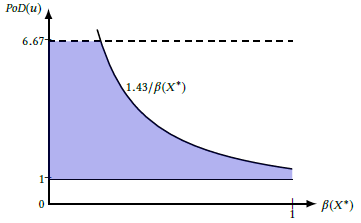
\includegraphics[scale=0.7]{figs/podbounds.png}
	\end{center}
	\caption{$\PoD$ vs disparity parameter for the HDB problem with current EIP quotas and ethnic proportions from Census 2010.\label{fig:PoDbeta}}
\end{wrapfigure}

\subsection{Experimental Analysis}\label{sec:experiments}
In this section, we present simulations of the \ASTC problem using recent, publicly available datasets: Singapore demographic and housing allocation statistics, and the Chicago public school admission data. 
We compare the welfare of three assignment mechanisms: unconstrained optimal (maximizing welfare while ignoring the diversity constraints), constrained optimal (finding the optimal allocation under diversity constraints), and one-shot lottery-based (running a lottery with diversity constraints, as is the case for the HDB mechanism).\footnote{We generated a uniformly random sequence over agents and assigned to each an item for which it has the highest utility among unassigned items in blocks for which that agent's ethnicity quota had not been filled yet. We abstract away other complications of actual lottery-based approaches used in our problem domains to focus on diversity constraints.} Conducting large-scale surveys to elicit agent preferences over items was beyond the scope of this work, so we simulated utilities based on reasonable models for both problems. We solved both the unconstrained and constrained social welfare maximizations using the Gurobi Optimizer. We refer the reader to \url{https://git.io/fNhhm} for full implementation details. 
\begin{wrapfigure}[25]{R}{0.35\textwidth}
	\vspace{-12pt}
	\begin{center}
		\begin{tabular}[t]{c}
			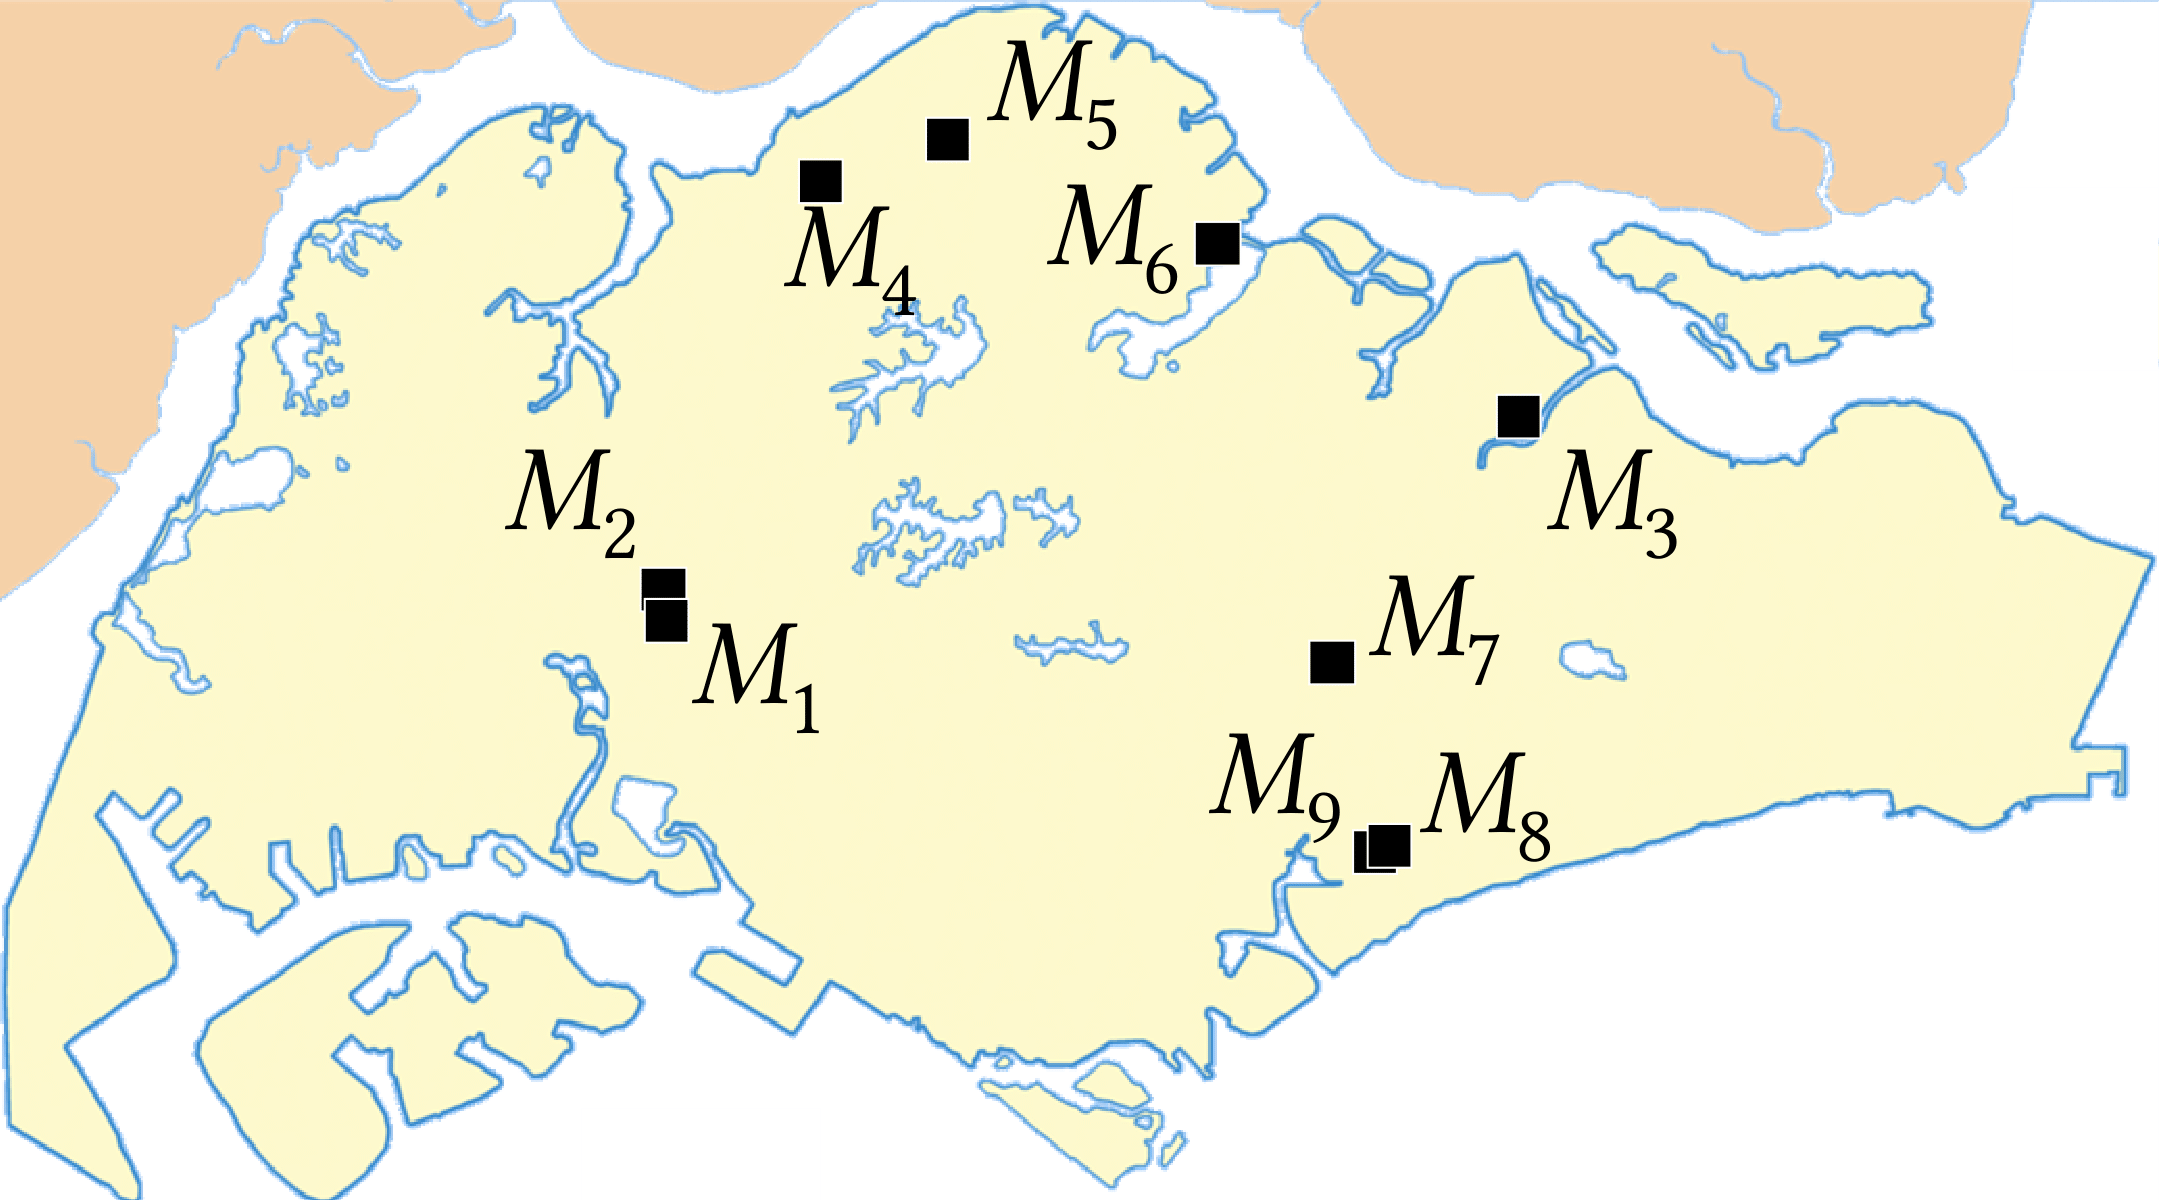
\includegraphics[scale=0.057]{figs/Map01Final081.png}\\ 
			(a)\\
			\\
			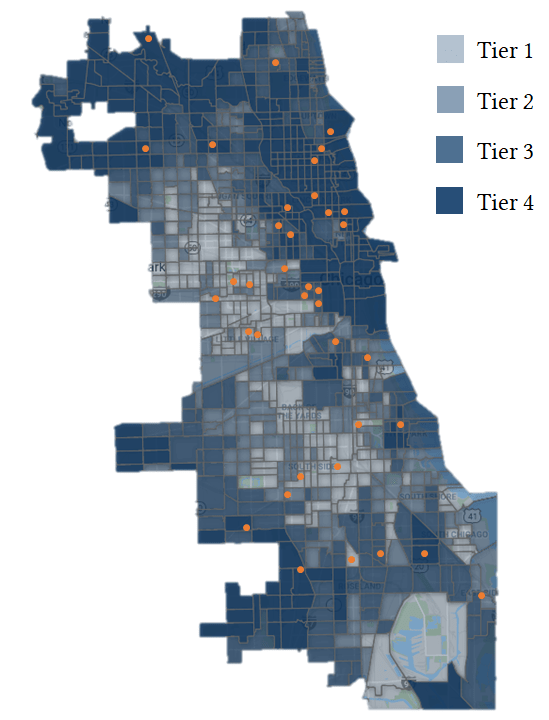
\includegraphics[scale=0.19]{figs/Chicago_Tier_School.png}\\
			(b)
		\end{tabular}
	\end{center}
	\caption{(a) Singapore public housing block locations. (b) Tier statuses of Chicago census tracts and magnet school locations (orange dots). \label{figMap}}
\end{wrapfigure}
\paragraph{The Singapore Public Housing Allocation Problem.} 
We collected data on the locations and numbers of flats of recent HDB housing development projects advertised over the second and third quarters of 2017.\footnote{\url{http://www.hdb.gov.sg/cs/infoweb/residential/buying-a-flat/new/bto-sbf}} 
Each development constitutes a block in our simulations, for a total of $m = 1350$ flats partitioned into $l = 9$ blocks $M_1, \ldots, M_9$ (Figure \ref{figMap}(a)), consisting of 128, 162, 156, 249, 108, 94, 104, 190, 159 flats respectively. There are pre-specified \emph{categories} of flats, viz. 2-room flexi, 3-room, 4-room, and 5-room; our data set includes lower and upper bounds, $\LB(t,q)$ and $\UB(t,q)$ respectively, on the monthly cost (loan) for a flat of category $t$ in block $M_q$ for every $t$ and $q$.
We simulate $2$ pools of $n$ applicants whose ethnic composition follows the 2010 Singapore census report \cite{Sing2010}, as shown in Table~\ref{SGtable}.
\begin{wraptable}{O}{0.3\textwidth}
	\begin{tabular}{|c|c|c|c|}
		\hline
		$n$ & $|N_1|$& $|N_2|$ & $|N_3|$ \\ \hline
		$1350$ & $1000$ & $180$ & $170$\\
		$3000$ & $2223$ & $402$ & $375$\\ \hline
	\end{tabular}
\caption{$\#$applicants (types $1$, $2$, and $3$ are Chinese, Malay, Indian/Others respectively)\label{SGtable}}
\end{wraptable}
From the same census report, we collected the average salary $S(p)$ of each ethnicity group $p \in [k]$, given in Singapore dollars: $S(1) = S\$7,326$, $S(2)=S\$4,575$ and $S(3) = S\$7,664$. 
From publicly available data\footnote{\url{https://data.gov.sg/dataset/master-plan-2014-planning-area-boundary-web}} on Singapore's Master Plan 2014,\footnote{\url{https://www.ura.gov.sg/Corporate/Planning/Master-Plan/}} we glean the locations of the geographic centers of the $55$ planning areas that Singapore is divided into; we also obtained the population sizes of the three ethnicity groups under consideration in each planning area from the General Household Survey 2015 data available from the Department of Statistics, Singapore.\footnote{\url{https://www.singstat.gov.sg/publications/ghs/ghs2015content}}
Our block capacities follow latest HDB block quotas~\cite{deng2013publichousing}: $\alpha_{1q} = 0.87, \alpha_{2q} = 0.25$, $\alpha_{3q} = 0.15$ for every block $M_q$. 

We simulate $4$ utility models; each has one parameter that does not come from the data: \textbf{(i) {\em Distance-based} ($\Dist(\sigma^2)$)}: Each agent $i \in N$ has a preferred geographic location $\vec a_i \in \R^2$ (chosen uniformly at random within the physical landmass of Singapore) that she would like to live as close as possible to (say, the location of her parents' apartment, workplace, or preferred school). For every block $M_q$, we generate the utility of that agent $i$ for apartment $j \in M_q$ by first drawing a sample from the normal distribution $\mathcal{N}(1/ d(\vec a_i,\loc(M_q)),\sigma^2)$, where $\loc(M_q) \in \R^2$ is the geographical location of block $M_q$ and $d(\cdot,\cdot)$ represents Euclidean distance, and then renormalizing to make the sum of utilities of each agent for all apartments in $M$ equal to 1. \textbf{(ii) {\em Type-based} ($\Ethn(\sigma^2)$)}: We assume that all agents of the same type (i.e., ethnic group) have the same preferred location (i.e.,  $\forall p \in [k], \forall i,i' \in N_p, \vec a_i = \vec a_{i'}$); the rest is similar to the above distance-based model. \textbf{(iii) {\em Project approval-based} ($\Proj(\rho)$)}: We construct, for each type, a categorical distribution over the $55$ planning areas of Singapore, the probability of each area being proportional to the fraction of the sub-population of that type living in that area; for each agent $i$, we sample a preferred planning area from the above distribution corresponding to $i$'s type; if a project $M_q$ is within a radius $\rho$ of the geographic center of agent $i$'s preferred planning area, then $i$ approves of the project i.e., $u(i,j) = 1$ $\forall j \in M_q$, else $i$ disapproves of the project i.e., $u(i,j) = 0$ $\forall j \in M_q$. \textbf{(iv) {\em Price-based} ($\Price(\sigma^2)$)}: Each agent $i \in N_p$ has a salary $s_i$ that is generated according to the normal distribution $\mathcal{N}(S(p),\sigma^2)$. Each flat $j \in M_q$ of category $t$ has a monthly cost $p_j$ chosen uniformly in $[\mathit{LB}(t,q), \mathit{UB}(t,q)]$. 
The utility that agent $i$ derives from flat $j$ is then defined by $u(i,j)= 1/(p_j - \frac{s_i}{3})^2$, assuming that agent $i$ is willing to pay one-third of her monthly salary on mortgage installments;\footnote{Inspired by the Singapore Central Provident Fund Board-endorsed ``3-3-5 rule", as of 21 Sep 2017.} the rationale for the utility formula is that a high cost relative to the budget makes flats unaffordable, while a much lower cost indicates unsatisfactory quality, making the agent unhappy in both scenarios. 

For each of our treatments (Figures~\ref{figTests1}--\ref{figTests3}), we plot the realized $\PoD(u)$ (hatched bar), the theoretical upper bound on $\PoD(u)$ as per Theorem~\ref{thm_parampod} (dark gray bar), and the relative loss of the HDB lottery mechanism (i.e., the ratio of $\OPT(u)$ to the total utility of the assignment produced by the lottery mechanism) averaged over 100 agent permutations (light gray bar) against the values of the corresponding model parameters ($\sigma^2$ or $\rho$). 
In order to compare $\Dist(\sigma^2)$ with $\Ethn(\sigma^2)$, we vary both $\sigma^2$ in $\{1,5,10\}$ and $n$ in $\{1350, 3000\}$; 
the results reported in Figures~\ref{figTests1} are on average performance over $100$ randomly generated instances. 
Our first observation is that, in all our experiments, $\Dist(\sigma^2)$ exhibits virtually no utility loss due to the imposition of type-block constraints (see the hatched bars in Figures~\ref{figTests1}(a)). 
This is because utilities in $\Dist(\sigma^2)$ are independent of ethnicity, resulting in a very low value for the inter-type disparity parameter $\beta$ (indicated by the dark gray bars) --- in fact, for any utility model where utilities are independent of ethnicity, the expected value of the disparity parameter is $1$. 
For the $\Ethn(\sigma^2)$ model-based utilities, the disparity parameter is somewhat higher (utilities do strongly depend on ethnicity), resulting in a higher $\PoD(u)$ (see the hatched bars in Figures~\ref{figTests1}(b)). 
\begin{figure}[t]
	\begin{center}
		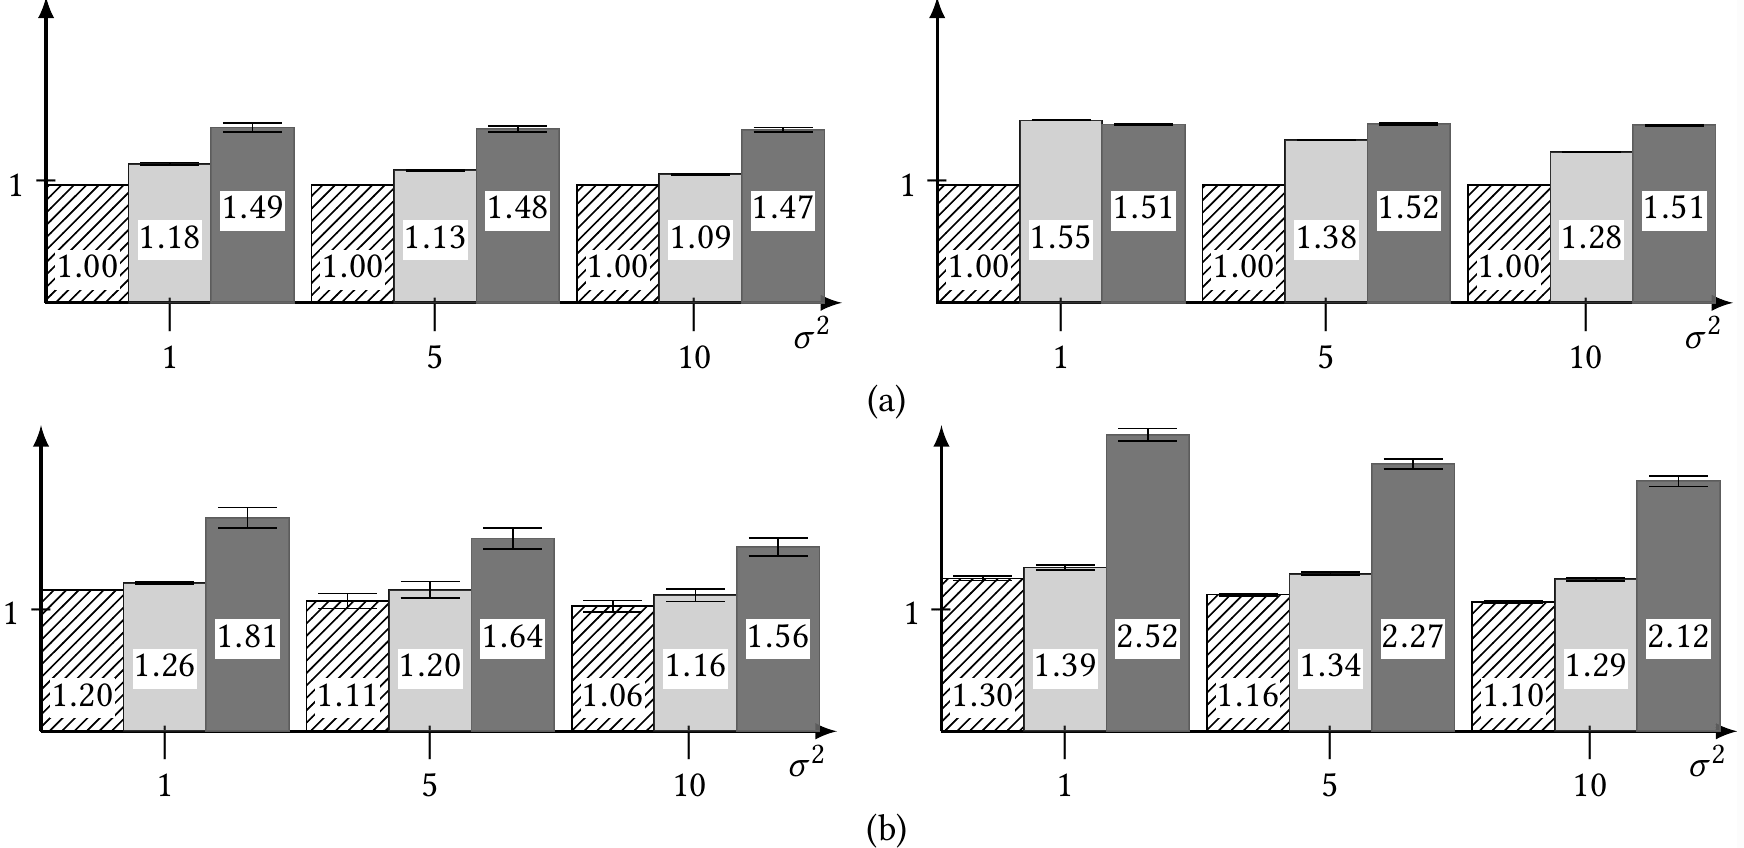
\includegraphics[scale=0.21]{figs/sing1.png}
	\end{center}
	\caption{Averaged utility losses for (a) $\Dist(\sigma^2)$ and (b) $\Ethn(\sigma^2)$ with $n = m = 1350$ (left) and $n = 3000$, $m = 1350$ (right). \label{figTests1}}
\end{figure}
Despite making no attempt to optimize social welfare under type-block constraints, the HDB lottery mechanism does surprisingly well when the number of agents equals the number of apartments (see the light gray bars in the left part of Figure~\ref{figTests1}), extracting at least $84\%$ of the optimal unconstrained welfare under the $\Dist(\sigma^2)$ utility model, and at least $79\%$ of the social welfare under the $\Ethn(\sigma^2)$ model. 
However, the lottery-induced welfare is negatively impacted by the number of agents (see the light gray bars in the right part of Figure~\ref{figTests1}); 
for instance, it only extracts $65\%$ of the optimal unconstrained welfare under $\Dist(1)$ with $n=3000$ and, in fact, the lottery-induced welfare loss for this treatment even exceeds the theoretical upper bound on the price of diversity.

For $\Proj(\rho)$, we use the fact that one degree of latitude or longitude at the location of Singapore corresponds to roughly 111 km to compute distances; we vary $\rho$ in $\{5,7.5,10\}$ (in km). The results averaged over 100 runs are provided in Figure~\ref{fig:ProjApprov}. In all instances, $\PoD(u)$ is almost one and the lottery-induced welfare is also nearly as good, achieving at least $87\%$ of the unconstrained optimum for $1350$ agents and practically $100\%$ for $3000$ agents; the disparity parameter is also consistently close to its ideal value of $1$, keeping the upper bound at around $1.45$ regardless of the radius. Thus, this can be considered an example of a utility model for which the lottery mechanism virtually implements a constrained optimal allocation for a wide range of model parameters.
\begin{figure}[t]
	\begin{center}
		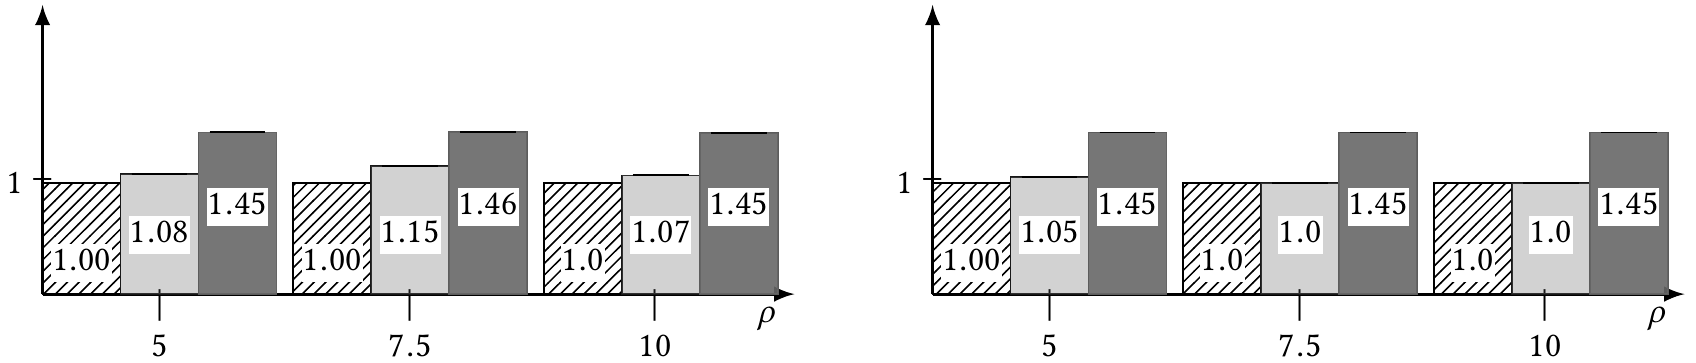
\includegraphics[scale=0.21]{figs/sing2.png}
	\end{center}
	\caption{Averaged utility losses for $\Proj(\rho)$ with $n = m = 1350$ (left) and $n = 3000$, $m = 1350$ (right). \label{fig:ProjApprov}}
\end{figure}
Finally, for $\Price(\sigma^2)$, we  vary $\sigma^2$ in $\{0,10,50\}$; the results obtained by averaging over 100 runs are given in Figure~\ref{figTests3}.
While the price of diversity is practically equal to one in all instances, the welfare loss observed with the lottery mechanism drastically increases with $\sigma^2$ (recall that agents from the same ethnicity group have identical preferences when $\sigma^2 = 0$): for instance, for $1350$ agents, it extracts $98\%$ of the optimal unconstrained welfare under $\Price(0)$ while it only extracts $35\%$ of this value under $\Price(50)$. 
%Moreover, for $\Price(50)$, %we found problem instances in which the the welfare loss induced by the lottery mechanism exceeds the corresponding theoretical upper bound on $\PoD(u)$.
%we observe that the welfare loss induced by the lottery mechanism exceeds the theoretical upper bound on $\PoD(u)$ in some instances with $1350$ agents. %(but this effect appears to be mitigated by a larger number of agents in our experiments). 
These numerical tests show that utility models exist for which the lottery mechanism may perform poorly compared to the optimal constrained allocation mechanism, even in allocation problems with a very low price of diversity.
\begin{figure}[t]
	\begin{center}
		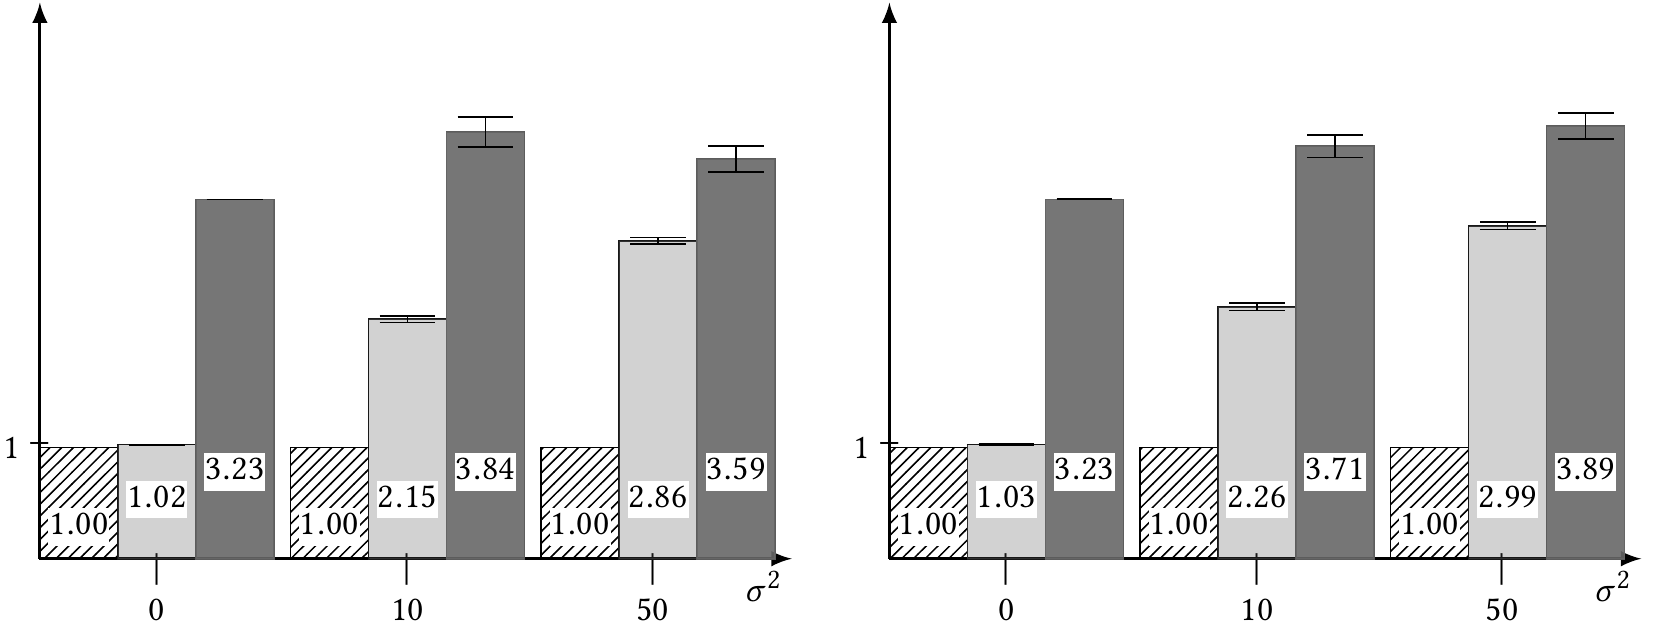
\includegraphics[scale=0.21]{figs/sing3.png}
	\end{center}
	\caption{Averaged utility losses for $\Price(\sigma^2)$ with $n = m = 1350$ (left) and $n = 3000$, $m = 1350$ (right). \label{figTests3}}
\end{figure}
\paragraph{Chicago Public School Admissions.} Chicago Public Schools (CPS) is one of the largest school districts in the U.S.A.,\footnote{\url{http://www.cps.edu/About_CPS/At-a-glance/Pages/Stats_and_facts.aspx}} overseeing more than 600 schools of various types.\footnote{\url{http://cpstiers.opencityapps.org/about.html}} The application and selection processes for these schools involve a number of computerized lotteries, 
with a significant number of entry-level seats in magnet and selective enrollment schools being filled by lotteries based on a \emph{tier system} based on the family \emph{socio-economic status} (SES) as part of a social integration policy. 
The city computes a multi-factor, composite SES score for each of the census tracts that Chicago is divided into, and places each tract in one of four tiers based on its score in such a way that each tier contains (roughly) a quarter of school-aged children. 
The tier of a child is determined by their residential address. 
Of the seats in each school earmarked for a \emph{citywide SES lottery} or \emph{general lottery}, an equal number is allocated to each tier, and there is an upper limit on the number of schools that a child may apply to (see \cite{schools2017chicago,quick2016chicago}). 
We apply our setup to a simplified version of the CPS student-seat allocation scenario.

We collected data from the Chicago Public Schools website\footnote{\url{http://cps.edu/Pages/home.aspx}} on the locations of magnet schools in Chicago (which use a lottery mechanism to select students), as well as the total number of students enrolled in these schools in 2018, which we divided by $9$ to obtain the approximate number of first-graders (there are nine grades in total). 
This leads us to instances with $l=37$ blocks (schools) and $m = 2261$ items (available seats) in total. 
In this school admission problem, students are partitioned into $k=4$ types, viz. Tiers 1, 2, 3 and 4, depending on their residence (see Figure \ref{figMap}(b)\footnote{Based on data from \url{http://cpstiers.opencityapps.org/} and \url{http://cps.edu/ScriptLibrary/Map-SchoolLocator/index.html}.}). In our experiments, we simulate $2$ pools of $n$ students where the type composition follows the real-world proportion, as shown in Table~\ref{Chictable}. Our type-block capacities are $\lambda_{pq} = 0.25 |M_q|$ for every pair $(p,q)$. For our student-seat utility simulations, we use the distance-based utility model $\Dist(\sigma^2)$ we introduced in the housing domain, with the following important modifications: 
we choose the preferred location of a student uniformly at random from the collection of census tracts (polygons) belonging to her tier (see Figure \ref{figMap}(b)), where the position of every polygon is approximated by taking the averaged coordinates of its extreme points; we reset each student's utility to $0$ for any school ranked $21$st or lower in the preference ordering induced by her utilities (since students are allowed to apply to at most 20 schools), and then renormalize the utilities.
\begin{wraptable}{l}{0.36\textwidth}
\begin{tabular}{|c|c|c|c|c|}
	\hline
	$n$ & $|N_1|$& $|N_2|$& $|N_3|$ & $|N_4|$\\ \hline
	$2261$ & $613$ & $622$ & $533$ & $493$\\
	$5000$ & $1355$ & $1375$ & $1180$ & $1090$\\ \hline
\end{tabular}
\caption{$\#$students (type $p$ is Tier $p$ for each $p \in [4]$.)\label{Chictable}}
\end{wraptable}

In our experiments, we vary $\sigma^2$ in $\{0,10,50\}$, and report 100-run averages of the same measurements as in the Singapore-based simulations (Figure \ref{figTests4}). We observe that both the price of diversity (hatched) and the loss of the lottery mechanism (light gray bar) decrease as $\sigma^2$ increases, remaining well below the Theorem~\ref{thm_parampod} bound (dark gray). However, the lottery mechanism loss is quite high in all instances and, just as in the Singapore case, gets worse for a higher number of students. Our experiments suggest that the lottery mechanism is better suited to problems with an equal number of agents and items.

\begin{figure}[t]
	\begin{center}
		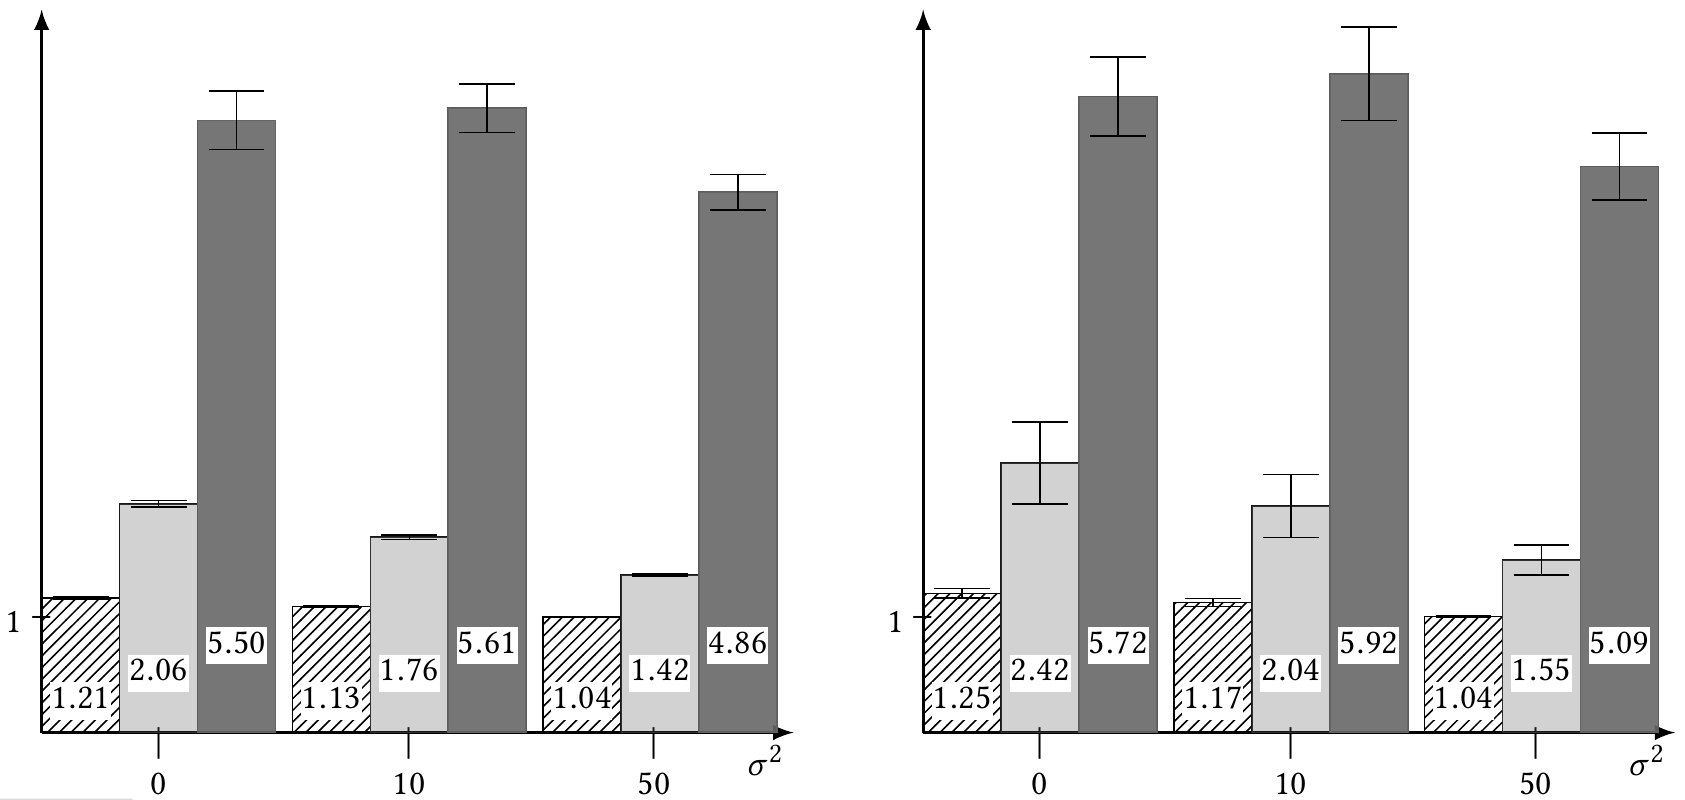
\includegraphics[scale=0.21]{figs/chicago.png}
	\end{center}
	\caption{Averaged utility losses for $\Dist(\sigma^2)$ with $n = m = 2261$ (left) and $n = 5000, m = 2261$ (right) in our Chicago-based simulations. \label{figTests4}}
\end{figure}

\section{Group Fairness in Allocation}\label{sec:grfair}
Up to this point, we have only explored the welfare loss due to capacity constraints; however, allocative efficiency is only one facet of group fairness. In some settings, groups might receive an overall worse outcome from the allocation mechanism, as compared to others. This is known in the fairness literature as {\em envy}. In this section, we explore how envy-freeness (i.e., having no agent group envy another's allocation) affects the allocation outcome.
We work with a model similar to that in Section~\ref{sec:assigntc} with two differences: (i) the items $M$ are not partitioned into blocks (or, equivalently, there is one block); (ii) we assume that for each agent $i \in N$ (resp. item $j \in M$), there is at least one item $j \in M$ (resp. agent $i \in N$) with $u(i,j)>0$. 
We adopt an alternative view of diversity-respecting assignment as a task of allocating bundles (i.e., disjoint subsets of $M$) to \emph{super-agents} (i.e., the types $N_1, \ldots, N_k$) in a manner that is both \emph{fair} and \emph{efficient} (see \cite{benabbou2019fairness} for further details and complete proofs). 

Each type $p$ is represented by a {\em super-agent}. We define $v_p(S)$, the \emph{valuation} of any super-agent $p \in [k]$ for any bundle of items $S \subseteq M$, as the maximum utilitarian social welfare of matching items in $S$ to agents of type $N_p$; $v_p(\cdot)$ is a monotonic, submodular set function (see \cite[Theorem 1]{benabbou2019fairness}). 
Moreover, our model does not satisfy the additive bundle-valuation assumption or the public goods assumption prevalent in most prior work (see e.g., \cite{caragiannis2016unreasonable,barman2018greedy,aleksandrov2018group,segal2018democratic} and references therein), necessitating novel solution techniques.
\begin{definition}[Allocation]\label{defn:alloc}
	An \emph{allocation} $\mathcal{A}$ is a collection of bundles $M^\mathcal{A}_1$,$ \cdots$, $M^\mathcal{A}_k$, such that $M^\mathcal{A}_1 \cup \ldots \cup M^\mathcal{A}_k \subseteq M$ and $M^\mathcal{A}_p \cap M^\mathcal{A}_q = \emptyset$ for all $p,q \in [k]$ with $p \neq q$, along with a maximum-$\USW$ matching between each type $N_p$ and its allocated bundle $M^\mathcal{A}_p$ for all $p \in [k]$, thereby inducing a unique $(N,M)$-matching $X^{\mathcal{A}} = (x^{\mathcal{A}}_{ij} )_{i \in N, j \in M}$.
\end{definition}
We call $M^\mathcal{A}_0 = M \backslash \cup_{p\in [k]} M^\mathcal{A}_p$ the set of \emph{withheld items} under allocation $\mathcal{A}$. In general, withholding items means that an allocation violates, by definition, the \emph{completeness} condition, a commonly used efficiency criterion. 
A type $p$'s \emph{marginal utility} for an item $j$ is the difference in $p$'s valuation of $S$ with and without item $j$: $\Delta_p(S;j) \triangleq v_p(S \cup \{j\}) - v_p(S)$ if $j \notin S$; $\Delta_p(S;j) \triangleq v_p(S) - v_p(S \backslash \{j\})$ if $j \in S$.
%\begin{align*}
%\Delta_p(S;j) \triangleq \begin{cases}
%v_p(S \cup \{j\}) - v_p(S)& \mbox{if }j \notin S\\ 
%v_p(S) - v_p(S \backslash \{j\})&\mbox{if }j \in S. 
%\end{cases}
%\end{align*}
We say that an item $j \in M^\mathcal{A}_p$ is \emph{unused} under $\mathcal{A}$ if it is either unassigned in the corresponding matching between $N_p$ and $M^\mathcal{A}_p$ or is assigned to an agent $i \in N_p$ such that $u(i,j)=0$. \emph{Cleaning} is the procedure of revoking all unused items from an allocation and putting them in the withheld set.
An item $j \in M$ is \emph{wasted} by an allocation $\mathcal{A}$ if it is either withheld (i.e., $j \in M^\mathcal{A}_0$) or allocated to a type $p$ and unused, although there is some other type $q$ with $\Delta_q(M^\mathcal{A}_q;j) > 0$. A {\em non-wasteful} allocation has no wasted items. Non-wastefulness is a reasonable efficiency concept in this setting; in fact, it turns out to be a relaxation (\cite[Lemma 1]{benabbou2019fairness}) of a popular efficiency criterion, \emph{Pareto optimality}: an allocation is Pareto optimal among types if the realized bundle-value of no type under this allocation can be strictly improved without strictly diminishing that of another.

We base our fairness criterion on the concept of \emph{envy}: a type $p$ envies a type $q$ if $v_p(M^\mathcal{A}_p) < v_p(M^\mathcal{A}_q)$; $p$ envies $q$ up to $\nu$ items, $\nu \in [|M^\mathcal{A}_q|]$, if there is a subset $C \subseteq M^\mathcal{A}_q$ of size $|C|=\nu$ such that $v_p(M^\mathcal{A}_p) \ge v_p(M^\mathcal{A}_q \backslash C)$ and, for every subset $C' \subseteq M^\mathcal{A}_q$ with $|C'| < \nu$, $v_p(M^\mathcal{A}_p) < v_p(M^\mathcal{A}_q \backslash C')$. Ideally, we want no type to envy another but such an allocation may not exist; a relaxation that always exists is the following:
\begin{definition}[Envy-freeness up to one item \cite{budish2011combinatorial}]\label{defn:tef1}
	Allocation $\mathcal{A}$ is \emph{envy-free up to one item} (EF1) among types if for any two types $p,q \in [k]$, $p$ either does not envy $q$ or envies $q$ up to one item i.e., there exists an item $j \in M^\mathcal{A}_q$ such that $v_p(M^\mathcal{A}_p) \ge v_p(M^\mathcal{A}_q \backslash \{j\})$.
\end{definition}
We want our allocation to be not just EF1 among types (thereby respecting diversity) but also efficient in one of the ways discussed above. Our first result in this vein applies to the \emph{binary utility model}: $u(i,j) \in \{0,1\}$, $\forall i \in N$, $\forall j \in M$.
This captures scenarios where each agent either approves or disapproves of an item but does not distinguish among its approved items.  %There exists prior work on fair allocation algorithms producing allocations with binary item utilities \cite{barman2018greedy} but most assume additive bundle valuations. 
Moreover, in formal conversations with stakeholders, we have found that a binary utility model is likely consistent with how agents value items in many real-world situations, e.g., in housing markets, a potential buyer might want a flat of a particular category only (such as a 3BHK within a 5-km radius of her workplace), being indifferent among flats of the same category.
\begin{theorem}\label{thm:bin_all}
	For any problem instance with a binary utility model, Algorithm~\ref{alg_bin} computes in $\poly(n,m)$ time an EF1 allocation that also maximizes the utilitarian social welfare of the induced $(N,M)$-matching.
\end{theorem}
\begin{algorithm}
	\DontPrintSemicolon
	\caption{Maximum-size Matching with Envy-Induced Transfers}\label{alg_bin}
	
	Compute a maximum-size matching of bipartite graph $(N,M)$ such that there is an edge between $i$ and $j$ iff $u(i,j)=1$, and clean the resulting allocation; designate the subset of items matched to agents in $N_p$ as type $p$'s allocated bundle $M^\mathcal{A}_p$ $\forall p \in [k]$. \label{MM}\\						
	\textbf{/*Envy-Induced Transfers*/}\\
	\While{there are two types $p,q$ such that $p$ envies $q$ up to more than $1$ item.}
	{
		Find item $j' \in M^\mathcal{A}_q$ such that $\Delta_p(M^\mathcal{A}_p;j')>0$.\\
		$M^\mathcal{A}_q \leftarrow M^\mathcal{A}_q \backslash \{j'\}$; $M^\mathcal{A}_p \leftarrow M^\mathcal{A}_p \cup \{j'\}$.\\
		Compute a maximum-size $(N_p,M_p)$-matching.
	}			
\end{algorithm}
It is easy to see that optimal utilitarian social welfare automatically implies Pareto optimality among types, and hence non-wastefulness. Thus, Algorithm~\ref{alg_bin} solves the fair and efficient allocation problem for binary utilities.

For more general utilities in $\R_+$, an algorithm that guarantees a similarly fair and efficient allocation remains elusive. 
However, we note that it is possible to obtain a type-complete TEF1 allocation in polynomial time by a natural extension (called {\bf L} hereafter) of the algorithm due to Lipton et al.~\cite{lipton2004approximately}: iterate over the items $j \in M$, giving item $j$ to a type, say $p$, that is currently not envied by any other type for its current bundle $M_p$; compute an optimal matching with the augmented bundle $M_p \cup \{j\}$; construct the \emph{envy graph} where there is a directed edge from a type $q$ to a type $r$ whenever $q$ envies $r$ and eliminate any cycle in this graph by transferring  the bundle of every type on this cycle to its predecessor on this cycle (to ensure that there is an unenvied type in each iteration), followed by re-matching within each such type. 
Although no item is withheld, it is possible for the final allocation to be wasteful: an item may be allocated to a type which has zero marginal utility for it or may \emph{become} unassigned after a bundle is transferred between types. 



One heuristic that could reduce waste is the following: %instead of giving an item to an \emph{arbitrary} unenvied type in each iteration, find 
in each iteration, find an item-type pair having the maximum marginal utility among all currently unenvied types and all unallocated items (breaking further ties uniformly at random, say), and allocate that item to that type. We call {\bf L}, augmented with this heuristic, {\bf H}. 
\begin{wraptable}[8]{l}[-3pt]{0.36\textwidth}
	\begin{tabular}{|c|c||c|c|}
		\cline{3-4}
		\multicolumn{2}{c}{}  & \multicolumn{2}{|c|}{$\%Waste$}\\ \hline 
		Data set & $\#$Items & {\bf L} & {\bf H}\\ \hline 
		\multirow{2}{*}{\textsc{Unequal}} & $50$ & $13\%$ & $0$ \\ \cline{2-4}
		& $100$ & $39\%$ & $0$ \\ \hline
		\multirow{2}{*}{\textsc{Equal}}  & $50$ & $0\%$ & $0$ \\ \cline{2-4}
		& $100$ & $0.005\%$ & $0$ \\ \hline
	\end{tabular}
\end{wraptable}
To test how this marginal utility maximization heuristic performs in practice, we experimentally compared procedures {\bf L} and {\bf H} using the percentage of items wasted averaged over runs, denoted by $\%Waste$, as our performance metric. We simulated two data sets with $n = 100$ agents partitioned into $k=3$ types: \textsc{Unequal} (ethnic proportions following Singapore 2010 census \cite{Sing2010}): $|N_1| = 74$, $|N_2| = 13$, $|N_3| = 13$; 
\textsc{Equal}: $|N_p| \approx n/k$ for all types $p \in [k]$. For each agent, we sampled $m$ numbers uniformly at random from $[0,1]$ and normalized them to generate utilities for all $m$ items, with $m \in \{50,100\}$. The results are shown in the adjoining table: the main observation is that {\bf H} produces \emph{zero} waste for \emph{all} experiments. Thus, augmenting {\bf L} with a simple heuristic produces a surprising improvement in performance over a wide range of problem parameters.   

\section{Discussion and future work}\label{sec:concl}
One of the extensions of the work presented here that we are currently pursuing is a rigorous analysis of the lottery mechanism with diversity quotas which we experimentally compared with our constrained optimization benchmark in Section~\ref{sec:experiments}. We are trying to assess whether certain lotteries are better than others in maintaining diverse but efficient outcomes in theory and in practice i.e., how the different parameters (the number of types, their respective percentage caps, sizes, and their utility structures) interact with the randomness of the draws to affect the welfare of the entire population as well as welfare-discrepancies among types. 

One other major direction we are investigating is an extension of/alternative to Algorithm~\ref{alg_bin} for arbitrary real-valued utilities. Several other possible approaches towards a tradeoff between fairness/diversity and efficiency are also worth exploring: diversity through the optimization of carefully constructed objective functions \cite{lang2016multi, ahmed2017diverse}; extensions of non-envy-based fairness concepts (group-wise egalitarian welfare, maximin shares \cite{barman2017approx,barman2018groupwise}, etc.) to our matching-based setting, and so on. 

\section*{Acknowledgments}\label{sec:acks}
Chakraborty and Zick are supported by Singapore NRF Fellowship R-252-000-750-733, and Benabbou by ANR project 14-CE24-0007-01-Cocorico-CoDec; a major part of the work was done when Benabbou was a post-doctoral research fellow at National University of Singapore (2017-18), supported by Singapore NRF Fellowship R-252-000-750-733. 
The authors would like to thank Xuan-Vinh Ho, Jakub Sliwinski (supported by MOE grant R-252-000-6255-133), and Edith Elkind as co-authors of publications on which this article is based, and Ayumi Igarashi for insightful discussions.
Thanks are also due to the anonymous reviewers of AAMAS 2018 and IJCAI 2019, and the attendees of COMSOC 2018 and FAMAS 2019 where parts of this work were presented. 

% ---- Bibliography ----
\begin{thebibliography}{10} 
	\itemsep=1pt 
	\begin{small}
		
		\bibitem{ahmed2017diverse} F.~Ahmed, J.~P.~Dickerson, and M.~Fuge. \newblock {Diverse Weighted Bipartite $b$-Matching.} \newblock {\em Proc. 26th IJCAI}, pp. 35--41, 2017.
		
		\bibitem{aleksandrov2018group} M.~Aleksandrov and T.~Walsh, Toby. \newblock Group envy freeness and group Pareto efficiency in fair division with indivisible items. \newblock {\em K{\"u}nstliche Intelligenz}, pp. 57--72, 2018.
		
		\bibitem{barman2017approx} S.~Barman and S.~K.~Krishnamurthy. \newblock Approximation Algorithms for Maximin Fair Division. \newblock {\em Proc. 18th EC}, pp. 647--664, 2017.
	
		\bibitem{barman2017finding} S.~Barman, S.~K.~Krishnamurthy, and R.~Vaish. \newblock Finding Fair and Efficient Allocations. \newblock {\em Proc. 19th EC}, pp. 557-574, 2018.
	
		\bibitem{barman2018greedy} S.~Barman, S.~K.~Krishnamurthy, R.~Vaish. \newblock Greedy algorithms for maximizing {N}ash social welfare. \newblock {\em Proc. 17th AAMAS}, pp. 7--13, 2018.
	
		\bibitem{barman2018groupwise} S.~Barman, A.~Biswas, S.~K.~Krishnamurthy, and Y.~Narahari. \newblock Groupwise maximin fair allocation of indivisible goods. \newblock {\em Proc. 32nd AAAI}, pp. 917--924, 2018.
	
		\bibitem{benabbou2017diversity} N.~Benabbou, M.~Chakraborty, X.~V.~Ho, J.~Sliwinski, and Y.~Zick. \newblock {Diversity Constraints in Public Housing Allocation.} \newblock {\em Proc. 17th AAMAS}, pp. 973--981, 2018.
	
		\bibitem{benabbou2019fairness} N.~Benabbou, M.~Chakraborty, E.~Elkind, and Y.~Zick. \newblock Fairness Towards Groups of Agents in the Allocation of Indivisible Items \newblock {\em Accepted to 28th IJCAI}, 2019.
	
		\bibitem{bouveret2016fair} S.~Bouveret, Y.~Chevaleyre, and N.~Maudet. \newblock {Fair Allocation of Indivisible Goods.} \newblock {\em Handbook of Computational Social Choice}, ed. F.~Brandt, V.~Conitzer, U.~Endriss, J.~Lang, and A.~D.~Procaccia, ch. 12, pp. 284--310, {Cambridge University Press}, 2016.
	
		\bibitem{bredereck2018multiwinner} R.~Bredereck, P.~Faliszewski, A.~Igarashi, M.~Lackner, and P.~Skowron. \newblock Multiwinner Elections with Diversity Constraints. \newblock {\em Proc. 32nd AAAI}, pp. 933--940, 2018.
	
		\bibitem{budish2011combinatorial} E.~Budish \newblock The combinatorial assignment problem: Approximate competitive equilibrium from equal incomes. \newblock {\em Journal of Political Economy}, University of Chicago Press, Vol. 119, No. 6, pp. 1061--1103, 2011.
	
		\bibitem{caragiannis2016unreasonable} I.~Caragiannis, D.~Kurokawa, H.~Moulin, A.~D.~Procaccia, N.~Shah, J.~Wang. \newblock The unreasonable fairness of maximum Nash welfare. \newblock {\em Proc. 17th EC}, pp. 305--322, 2016.
	
		\bibitem{chua1991race} B.~Chua. \newblock {Race relations and public housing policy in Singapore.} \newblock {\em {Journal of Architectural and Planning Research}}, pp. 343--354, 1991.
	
		\bibitem{deng2013publichousing} Y.~Deng, T.~F.~Sing, and C.~Ren \newblock {The story of Singapore's public housing: From a nation of home-seekers to a nation of homeowners.} \newblock {\em The Future of Public Housing: Ongoing Trends in the East and the West}, ed. J.~Chen, M.~Stephens, and Y.~Man, ch. 7, pp. 103--121, Springer, 2013. ISBN 978-3-642-41621-7.
	
		\bibitem{fain2016core} B.~Fain, A.~Goel, and K.~Munagala. \newblock {The core of the participatory budgeting problem.} \newblock {\em Proc. 12th WINE}, pp. 384--399, 2016.
	
		\bibitem{fragiadakis2017improving} D.~Fragiadakis and P.~Troyan. \newblock {Improving matching under hard distributional constraints.} \newblock {\em Theoretical Economics}, Wiley Online Library, Vol. 12, No. 2, pp. 863--908, 2017.
	
		\bibitem{HDB10PR} {Housing and Development Board, Singapore.} \newblock {Policy changes to support an inclusive and cohesive home [Press release]. 5 Mar 2010.} \newblock \url{http://www.nas.gov.sg/archivesonline/speeches/record-details/809e76bf-115d-11e3-83d5-0050568939ad.}
	
		\bibitem{HDB18keystats} {Housing and Development Board, Singapore.} \newblock {Annual Report 2016/2017: Key Statistics. 2017} \newblock \url{http://www10.hdb.gov.sg/ebook/AR2018/key-statistics.html}.
	
		\bibitem{kamada2015efficient} Y.~Kamada and F.~Kojima. \newblock Efficient matching under distributional constraints: Theory and applications. \newblock {\em American Economic Review}, Vol. 105, No. 1, pp. 67--99, 2015.
	
		\bibitem{kim2013singapore} S.~Y.~Phang and K.~Kim. \newblock {Singapore's Housing Policies: 1960-2013.} \newblock {\em {Frontiers in Development Policy: Innovative Development Case Studies}}, pp. 123--153, 2013.
	
		\bibitem{kuhn1955hungarian} H.~W.~Kuhn. \newblock {The Hungarian method for the assignment problem.} \newblock {\em Naval Research Logistics}, 2(1-2):83--97, 1955.
	
		\bibitem{kurokawa2016can} D.~Kurokawa, A.~D.~Procaccia, and J.~Wang. \newblock When can the maximin share guarantee be guaranteed? \newblock {\em Proc. 30th AAAI}, pp. 523--529, 2016.
	
		\bibitem{lang2016multi} J.~Lang and P.~K.~Skowron \newblock Multi-Attribute Proportional Representation. \newblock {\em Proc. 30th AAAI}, pp. 530--536, 2016.
	
		\bibitem{lipton2004approximately} R.~J.~Lipton, E.~Markakis, E.~Mossel, and A.~Saberi. \newblock {On approximately fair allocations of indivisible goods.} \newblock {\em Proc. 5th EC}, pp. 125--131, 2004.
	
		\bibitem{lovasz2009matching} L.~Lov{\'a}sz and M.~D.~Plummer. \newblock {Matching theory.} \newblock {\em {American Mathematical Society}}, Vol. 367, 2009. 
	
		\bibitem{munkres1957algo} J.~Munkres. \newblock Algorithms for the assignment and transportation problems. \newblock {\em Journal of SIAM}, Vol. 5, No. 1, pp. 32--38, 1957.
	
		\bibitem{Parl1989} {Parliament of Singapore.} \newblock {Better racial mix in HDB housing estates.} \newblock {Parliament Debates: Official Report. 16 Feb 1989. Vol. 52, cols. 650-668.}
	
		\bibitem{procaccia2014fair} A.~D.~Procaccia and J.~Wang. \newblock {Fair enough: Guaranteeing approximate maximin shares.} \newblock {\em Proc. 15th EC}, pp. 675--692, 2014.
	
		\bibitem{quick2016chicago} K.~Quick. \newblock Chicago Public Schools: Ensuring Diversity in Selective Enrollment and Magnet Schools. \newblock {\em The Century Foundation.}  \url{https://tcf.org/content/report/chicago-public-schools}, 14 Oct 2016.
	
		\bibitem{schools2017chicago} Chicago Public Schools \newblock Chicago Public Schools Policy Manual: Admissions Policy for Magnet, Selective Enrollment and Other Options For Knowledge Schools and Programs. \newblock Section 202.2. Board Report 17-0426-PO2. Available at \url{http://policy.cps.edu/Policies.aspx}, 26 Apr 2017.
	
		\bibitem{segal2018democratic} E.~Segal-Halevi and W.~Suksompong. \newblock Democratic Fair Allocation of Indivisible Goods. \newblock {\em Proc. 27th IJCAI}, pp. 482--488, 2018.
	
		\bibitem{sim2003public} L.~L.~Sim, S.~M.~Yu, and S.~S.~Han. \newblock {Public housing and ethnic integration in Singapore.} \newblock {\em {Habitat International}}, Vol. 27, No. 2, pp. 293--307, 2003.
	
		\bibitem{Sing2010} Department of Statistics, Singapore. \newblock {Singapore 2010 Census: Key Indicators of the Resident Population.} \newblock 2010.
	
		\bibitem{Sing2018} {Department of Statistics, Singapore.} \newblock {Singapore in Figures.} \newblock 2018.
	
		\bibitem{stoyanovich2018online} J.~Stoyanovich, K.~Yang, and H.V.~Jagadish. \newblock {Online set selection with fairness and diversity constraints.} \newblock {\em Proc. 21st EDBT}, pp. 241--252, 2018.
	
		\bibitem{USedu2017} {U.S. Department of Education, Office of Elementary and Secondary Education.} \newblock {Improving Outcomes for All Students: Strategies and Considerations to Increase Student Diversity.} \newblock Washington, D.C. \url{https://www.ed.gov/diversity-opportunity}, 19 Jan 2017.
	
		\bibitem{wong2014estimating} M.~Wong. \newblock {Estimating the distortionary effects of ethnic quotas in Singapore using housing transactions.} \newblock {\em Journal of Public Economics}, Vol. 115, pp. 131--145, 2014.
		
	\end{small} 
\end{thebibliography}

\end{document}
\end{article}


\begin{article}
{Towards Responsible Data-driven Decision Making in Score-Based Systems}
{Abolfazl Asudeh, H. V. Jagadish, Julia Stoyanovich}
\graphicspath{{submissions/Jagadish/}}
\pdfminorversion=5
\documentclass[11pt]{article}
\usepackage{deauthor,times,graphicx,caption,microtype}
\usepackage{hyperref}
\usepackage{listings}
\usepackage{booktabs}

\begin{document}

\title{Optimistic Lock Coupling: A Scalable and Efficient General-Purpose Synchronization Method}

\author{Viktor Leis, Michael Haubenschild\raisebox{0.9ex}{$\ast$}, Thomas Neumann\\ Technische Universit{\"a}t M{\"u}nchen \hspace{0.7cm} Tableau Software\raisebox{0.9ex}{$\ast$} \\ {\{leis,neumann\}{@}in.tum.de} \hspace{0.7cm} {mhaubenschild{@}tableau.com\raisebox{0.9ex}{$\ast$}}}

\maketitle

\begin{abstract}
As the number of cores on commodity processors continues to increase, scalability becomes more and more crucial for overall performance.
Scalable and efficient concurrent data structures are particularly important, as these are often the building blocks of parallel algorithms.
Unfortunately, traditional synchronization techniques based on fine-grained locking have been shown to be unscalable on modern multi-core CPUs.
Lock-free data structures, on the other hand, are extremely difficult to design and often incur significant overhead.

In this work, we make the case for Optimistic Lock Coupling as a practical alternative to both traditional locking and the lock-free approach.
We show that Optimistic Lock Coupling is highly scalable and almost as simple to implement as traditional lock coupling.
Another important advantage is that it is easily applicable to most tree-like data structures.
We therefore argue that Optimistic Lock Coupling, rather than a complex and error-prone custom synchronization protocol, should be the default choice for performance-critical data structures.
\end{abstract}

\section{Introduction}

% more and more cores
Today, Intel's commodity server processors have up to 28 cores and its upcoming microarchitecture will have up to 48 cores per socket~\cite{intel}.
Similarly, AMD currently stands at 32 cores and this number is expected to double in the next generation~\cite{amd}.
Since both platforms support simultaneous multithreading (also known as hyperthreading), affordable commodity servers (with up to two sockets) will soon routinely have between 100 and 200 hardware threads.

% data structure scalability is important
With such a high degree of hardware parallelism, efficient data processing crucially depends on how well concurrent data structures scale.
Internally, database systems use a plethora of data structures like table heaps, internal work queues, and, most importantly, index structures.
Any of these can easily become a scalability (and therefore overall performance) bottleneck on many-core CPUs.

% traditional synchronization: fine-grained locks, slow, cache invalidation
Traditionally, database systems synchronize internal data structures using fine-grained reader/writer locks\footnote{In this work, we focus on data structure synchronization rather than high-level transaction semantics and therefore use the term {\em lock} for what would typically be called {\em latch} in the database literature. We thus follow common computer science (rather than database) terminology.}.
Unfortunately, while fine-grained locking makes lock contention unlikely, it still results in bad scalability because lock acquisition and release require writing to shared memory.
Due to the way cache coherency is implemented on modern multi-core CPUs, these writes cause additional cache misses\footnote{The cache coherency protocol ensures that all copies of a cache line on other cores are invalidated before the write can proceed.} and the cache line containing the lock's internal data becomes a point of physical contention.
As a result, any frequently-accessed lock (e.g., the lock of the root node of a B-tree) severely limits scalability.

% lock-free bw-tree: no more latches, but indirections, extremely complex
Lock-free data structures like the Bw-tree~\cite{DBLP:conf/icde/LevandoskiLS13a} (a lock-free B-tree variant) or the Split-Ordered List~\cite{DBLP:journals/jacm/ShalevS06} (a lock-free hash table) do not acquire any locks and therefore generally scale much better than locking-based approaches (in particular for read-mostly workloads).
However, lock-free synchronization has other downsides:
First, it is very difficult and results in extremely complex and error-prone code (when compared to locking).
Second, because the functionality of atomic primitives provided by the hardware (e.g., atomically compare-and-swap 8 bytes) is limited, complex operations require additional indirections within the data structure.
For example, the Bw-tree requires an indirection table and the Split-Ordered List requires ``dummy nodes'', resulting in overhead due to additional cache misses.

% OLC for the win
In this paper we make the case for {\em Optimistic Lock Coupling (OLC)}, a synchronization method that combines some of the best properties of lock-based and lock-free synchronization.
OLC utilizes a special lock type that can be used in two modes:
The first mode is similar to a traditional mutex and excludes other threads by physically acquiring the underlying lock.
In the second mode, reads can proceed optimistically by validating a version counter that is embedded in the lock (similar to optimistic concurrency control).
The first mode is typically used by writers and the second mode by readers.
Besides this special lock type, OLC is based on the observation that optimistic lock validations can be interleaved/coupled---similar to the pair-wise interleaved lock acquisition of traditional lock coupling.
Hence, the name Optimistic Lock Coupling.

OLC has a number of desirable features:
\begin{itemize}
\item By reducing the number of writes to shared memory locations and thereby avoiding cache invalidations, it {\bf scales well} for most workloads.
\item In comparison to unsynchronized code, it requires few additional CPU instructions making it {\bf efficient}.
\item OLC is {\bf widely applicable} to different data structures. It has already been successfully used for synchronizing binary search trees~\cite{DBLP:conf/ppopp/BronsonCCO10}, tries~\cite{artsync}, trie/B-tree hybrids~\cite{DBLP:dblp_conf/eurosys/MaoKM12}, and B-trees~\cite{buzzword}.
\item In comparison to the lock-free paradigm, it is also {\bf easy to use} and requires few modifications to existing, single-threaded data structures.
\end{itemize}
Despite these positive features and its simplicity, OLC is not yet widely known.
The goal of this paper is therefore to popularize this simple idea and to make a case for it.
We argue that OLC deserves to be widely known.
It is a good default synchronization paradigm---more complex, data structure-specific protocols are seldom beneficial.

The rest of the paper is organized as follows.
Section~\ref{sec:related} discusses related work, tracing the history of OLC and its underlying ideas in the literature.
The core of the paper is Section~\ref{sec:olc}, which describes the ideas behind OLC and how it can be used to synchronize complex data structures.
In Section~\ref{sec:evaluation} we experimentally show that OLC has low overhead and scales well when used to synchronize an in-memory B-tree.
We summarize the paper in Section~\ref{sec:conc}.

\newpage
\section{Related Work}\label{sec:related}

Lock coupling has been proposed as a method for allowing concurrent operations on B-trees in 1977~\cite{DBLP:journals/acta/BayerS77}.
This traditional and still widely-used method, described in detail in Graefe's B-tree survey~\cite{DBLP:journals/ftdb/Graefe11}, is also called ``latch coupling'', ``hand-over-hand locking'', and ``crabbing''.
Because at most two locks are held at-a-time during tree traversal, this technique seemingly allows for a high degree of parallelism---in particular if read/write locks are used to enable inner nodes to be locked in shared mode.
However, as we show in Section~\ref{sec:evaluation}, on modern hardware lock acquisition (even in shared mode) results in suboptimal scalability.

An early alternative from 1981 is a B-tree variant called B-link tree~\cite{DBLP:journals/tods/LehmanY81}, which only holds a single lock at a time.
It is based on the observation that between the release of the parent lock and the acquisition of the child lock, the only ``dangerous'' thing that could have happened is the split of a child node (assuming one does not implement merge operations).
Thus, when a split happens, the key being searched might end up on a neighboring node to the right of the current child node.
A B-link tree traversal therefore detects this condition and, if needed, transparently proceeds to the neighboring node.
Releasing the parent lock early is highly beneficial when the child node needs to be fetched from disk.
For in-memory workloads, however, the B-link tree has the same scalability issues as lock coupling (it acquires just as many locks).

The next major advance, Optimistic Latch-Free Index Traversal (OLFIT)~\cite{DBLP:conf/vldb/ChaHKK01}, was proposed in 2001.
OLFIT introduced the idea of a combined lock/update counter, which we call {\em optimistic lock}. % , for lack of a better name,
Based on these per-node optimistic locks and the synchronization protocol of the B-link tree, OLFIT finally achieves good scalability on parallel processors.
The OLFIT protocol is fairly complex, as it requires both the non-trivial B-link protocol and optimistic locks.
Furthermore, like the B-link tree protocol, it does not support merging nodes, and is specific to B-trees (cannot easily be applied to other data structures).

In the following two decades, the growth of main-memory capacity led to much research into other data structures besides the venerable B-tree.
Particularly relevant for our discussion is Bronson et al.'s~\cite{DBLP:conf/ppopp/BronsonCCO10} concurrent binary search tree, which is based on optimistic version validation and has a sophisticated, data structure-specific synchronization protocol.
To the best of our knowledge, this 2010 paper is the first that, as part of its protocol, interleaves version validation across nodes---rather than validating each node separately like OLFIT.
In that paper, this idea is called ``hand-over-hand, optimistic validation'', while we prefer the term Optimistic Lock Coupling to highlight the close resemblance to traditional lock coupling.
Similarly, Mao et al.'s~\cite{DBLP:dblp_conf/eurosys/MaoKM12} Masstree (a concurrent hybrid trie/B-tree) is also based on the same ideas, but again uses them as part of a more complex protocol.

The Adaptive Radix Tree (ART)~\cite{art} is another recent in-memory data structure, which we proposed in 2013.
In contrast to the two data structures just mentioned, it was originally designed with single-threaded performance in mind without supporting concurrency.
To add support for concurrency, we initially started designing a custom protocol called Read-Optimized Write Exclusion (ROWEX)~\cite{artsync}, which turned out to be non-trivial and requires modifications of the underlying data structure\footnote{Note that ROWEX is already easier to apply to existing data structures than the lock-free approach. The difficulty depends on the data structure. Applying ROWEX is hard for B-trees with sorted keys and fairly easy for copy-on-write data structures like the Height Optimized Trie~\cite{hot}---with ART being somewhere in the middle.}.
However, fairly late in the project, we also realized, that OLC {\em alone} (rather than as part of a more complex protocol) is sufficient to synchronize ART.
No other changes to the data structure were necessary.
Both approaches were published and experimentally evaluated in a followup paper~\cite{artsync}, which shows that, despite its simplicity, OLC is efficient, scalable, and generally outperforms ROWEX.

Similar results were recently published regarding B-trees~\cite{buzzword}.
In this experimental study a simple OLC-based synchronization outperformed the Bw-tree~\cite{DBLP:conf/icde/LevandoskiLS13a}, a complex lock-free synchronization approach.
Another recent paper shows that for write-intensive workloads, locking often performs better than lock-free synchronization~\cite{DBLP:conf/cidr/FaleiroA17}.
These experiences indicate that OLC is a general-purpose synchronization paradigm and motivate the current paper.

%foster b-tree\cite{DBLP:journals/tods/GraefeKK12}
%Shasha theory~\cite{DBLP:journals/tods/ShashaG88}

\section{Optimistic Lock Coupling}\label{sec:olc}

% locks suck
The standard technique for inter-thread synchronization is mutual exclusion using fine-grained locks.
In a B-tree, for example, every node usually has its own associated lock, which is acquired before accessing that node.
The problem of locking on modern multi- and many-core processors is that lock acquisition and release require writing to the shared memory location that implements the lock.
This write causes exclusive ownership of the underlying cache line and invalidates copies of it on all other processor cores.
For hierarchical, tree-like data structures, the lock of the root node becomes a point of physical contention---even in read-only workloads and even when read/write locks are used.
Depending on the specific data structure, number of cores, cache coherency protocol implementation, cache topology, whether Non-Uniform Memory Access (NUMA) is used, locking can even result in multi-threaded performance that is worse than single-threaded execution.

% in b-trees this happens very much
The inherent pessimism of locking is particularly unfortunate for B-trees:
Despite the fact that logical modifications of the root node are very infrequent, every B-tree operation must lock the root node during tree traversal\footnote{To a lesser extent this obviously applies to all inner nodes, not just the root.}.
Even the vast majority of update operations (with the exception of splits and merges), only modify a single leaf node.
These observations indicate that a more optimistic approach, which does not require locking inner nodes, would be very beneficial for B-trees.

\subsection{Optimistic Locks}

% optimism to the rescue
As the name indicates, optimistic locks try to solve the scalability issues of traditional locks using an optimistic approach.
Instead of always physically acquiring locks, even for nodes that are unlikely to be modified simultaneously, after-the-fact validation is used to detect conflicts.
This is done by augmenting each lock with a version/update counter that is incremented on every modification.
Using this version counter, readers can optimistically proceed before validating that the version did not change to ensure that the read was safe.
If validation fails, the operation is restarted.

% details on opt locks
Using optimistic locks, a read-only node access (i.e., the majority of all operations in a B-tree) does not acquire the lock and does not increment the version counter.
Instead, it performs the following steps:
\begin{enumerate}
\item read lock version (restart if lock is not free)
\item access node
\item read the version again and validate that it has not changed in the meantime
\end{enumerate}
If the last step (the validation) fails, the operation has to be restarted.
Write operations, on the other hand, are more similar to traditional locking:
\begin{enumerate}
\item acquire lock (wait if necessary)
\item access/write to node
\item increment version and unlock node
\end{enumerate}
Writes can therefore protect a node from other writes.

% similar to locks
As we observed in an earlier paper~\cite{artsync}, because of similar semantics, optimistic locks can be hidden behind an API very similar to traditional read/write locks.
Both approaches have an exclusive lock mode, and acquiring a traditional lock in shared mode is analogous to optimistic version validation.
Furthermore, like with some implementations of traditional read/write locks, optimistic locks allow upgrading a shared lock to an exclusive lock.
Lock upgrades are, for example, used to avoid most B-tree update operations from having to lock inner nodes.
In our experience, the close resemblance of optimistic and traditional locks simplifies the reasoning about optimistic locks;
one can apply similar thinking as in traditional lock-based protocols.

\subsection{Lock Coupling with Optimistic Locks}

\begin{figure}
  \centering
  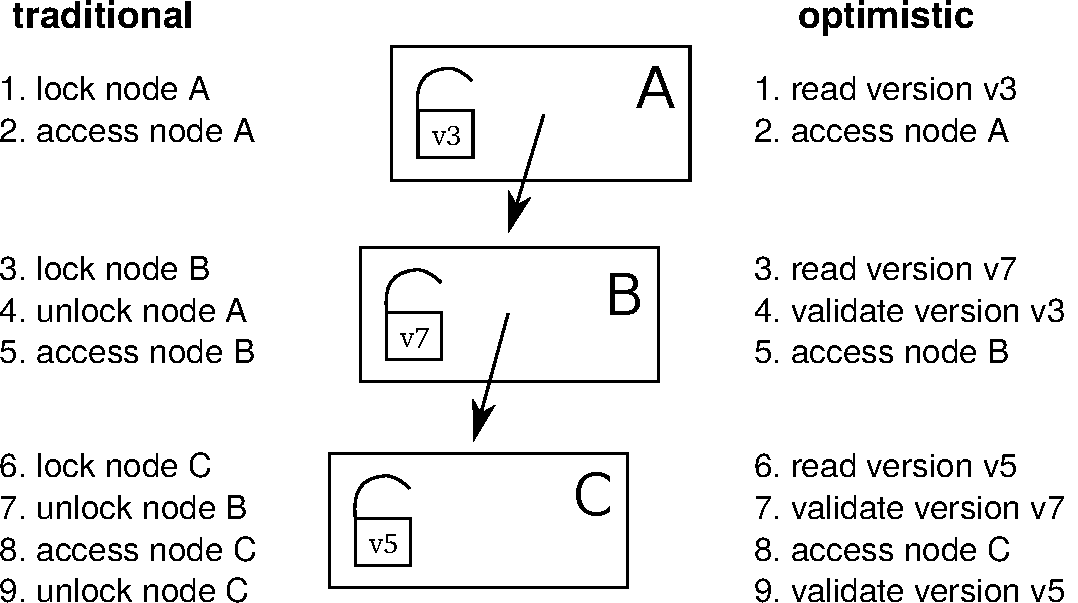
\includegraphics[width=0.65\linewidth]{olcall.pdf}
  \vspace{0.2cm}
  \caption{Comparison of a lookup operation in a 3-level tree using traditional lock coupling (left-hand side) vs.~optimistic lock coupling (right-hand side).}
  \label{fig:olc}
\end{figure}

The traditional and most common lock-based synchronization protocol for B-trees is lock coupling, which interleaves lock acquisitions while holding at most two locks at a time.
If, as we observed earlier, optimistic locks have similar semantics as traditional locks, it is natural to ask whether lock coupling can be combined with optimistic locks.
And indeed the answer is yes: One can almost mechanically translate traditional lock coupling code to optimistic lock coupling code.
This is illustrated in Figure~\ref{fig:olc}, which compares the traversal in a tree of height 3 using traditional and optimistic locks.
As the figure shows, the main difference is that locking is translated to reading the version and that unlocking becomes validation of the previously read version.
This simple change provides efficient lock-free tree traversal without the need to design a complex synchronization protocol.

It is important to emphasize the conceptual simplicity of OLC in comparison to data structures that use custom protocols like the Bw-tree~\cite{DBLP:conf/icde/LevandoskiLS13a}.
To implement lock-free access, the Bw-tree requires an indirection table, delta nodes, complex splitting and merging logic, retry logic, etc.
OLC, on the other hand, can directly be applied to B-trees mostly by adding the appropriate optimistic locking code and without modifying the node layout itself.
Therefore, OpenBw-Tree, an open source implementation of the Bw-tree, requires an order of magnitude more code than a B-tree based on OLC\footnote{Both implementations are available on GitHub: \url{https://github.com/wangziqi2016/index-microbench}}.
Given how difficult it is to develop, validate, and debug lock-free code, simplicity is obviously a major advantage.

\subsection{Correctness Aspects}

\begin{figure}
  % \centering
  %[basicstyle=\normalsize\ttfamily,showstringspaces=false,columns=fullflexible,breaklines=false,breakatwhitespace=true,numbers=none,numberstyle=\small,style=C,keepspaces=true]
\begin{lstlisting}[basicstyle=\ttfamily,language=C++,numbers=left,numberstyle=\small]
std::atomic<BTreeNode*> root;

// search for key in B+tree, returns payload in resultOut
bool lookup(Key key, Value& resultOut) {
   BTreeNode* node = root.load();
   uint64_t nodeVersion = node->readLockOrRestart();
   if (node != root.load()) // make sure the root is still the root
      restart();

   BTreeInner<Key>* parent = nullptr;
   uint64_t parentVersion = 0;

   while (node->isInner()) {
      auto inner = (BTreeInner*)node;

      // unlock parent and make current node the parent
      if (parent)
         parent->readUnlockOrRestart(parentVersion);
      parent = inner;
      parentVersion = nodeVersion;

      // search for next node
      node = inner->findChild(key);
      // validate 'inner' to ensure that 'node' pointer is valid
      inner->checkOrRestart(nodeVersion);
      // now it safe to dereference 'node' pointer (read its version)
      nodeVersion = node->readLockOrRestart();
   }

   // search in leaf and retrieve payload
   auto leaf = (BTreeLeaf*)node;
   bool success = leaf->findValue(key, resultOut);

   // unlock everything
   if (parent)
      parent->readUnlockOrRestart(parentVersion);
   node->readUnlockOrRestart(nodeVersion);

   return success;
}
\end{lstlisting}
  \vspace{0.2cm}
  \caption{B-tree lookup code using OLC. For simplicity, the restart logic is not shown.}
  \label{fig:lookup}
\end{figure}

So far, we have introduced the high-level ideas behind OLC and have stressed its similarity to traditional lock coupling.
Let us now discuss some cases where the close similarity between lock coupling and OLC breaks down.
To make this more concrete, we show the B-tree lookup code in Figure~\ref{fig:lookup}.
In the code, \texttt{readLockOrRestart} reads the lock version and \texttt{readUnlockOrRestart} validates that the read was correct.

One issue with OLC is that any pointer speculatively read from a node may point to invalid memory (if that node is modified concurrently).
Dereferencing such a pointer (e.g., to read its optimistic lock), may cause a segmentation fault or undefined behavior.
In the code shown in Figure~\ref{fig:lookup}, this problem is prevented by the extra check in line 25, which ensures that the read from the node containing the pointer was correct.
Without this additional validation, the code would in line 27 dereference the pointer speculatively read in line 23.
Note that the implementation of \texttt{checkOrRestart} is actually identical to \texttt{readUnlockOrRestart}.
We chose to give it a different name to highlight the fact that this extra check would not be necessary with read/write locks.

Another potential issue with optimistic locks is code that does not terminate.
Code that speculatively accesses a node, like an intra-node binary search, should be written in a way such that it always terminates---even in the presence of concurrent writes.
Otherwise, the validation code that detects the concurrent write will never run.
The binary search of a B-tree, for example, needs to be written in such a way that each comparison makes progress.
For some data structures that do not require loops in the traversal code (like ART) termination is trivially true.

\subsection{Implementation Details}

% implementation, efficiency
To implement an optimistic lock, one can combine the lock and the version counter into a single 64-bit\footnote{Even after subtracting one bit for the lock status, a back-of-the-envelope calculation can show that 63 bits are large enough to never overflow in practice.} word~\cite{artsync}.
A typical read operation will therefore merely consist of reading this version counter atomically.
In C++11 this can be implemented using the \texttt{std::atomic} type.

On x86, atomic reads are cheap because of x86's strong memory order guarantees.
No memory fences are required for sequentially-consistent loads, which are translated (by both GCC and clang) into standard \texttt{MOV} instructions.
Hence, the only effect of \texttt{std::atomic} for loads is preventing instruction re-ordering.
This makes version access and validation cheap.
Acquiring and releasing an optimistic lock in exclusive mode has comparable cost to a traditional lock:
A fairly expensive sequentially-consistent store is needed for acquiring a lock, while a standard \texttt{MOV} suffices for releasing it.
A simple sinlock-based implementation of optimistic locks can be found in the appendix of an earlier paper~\cite{artsync}.

OLC code must be able to handle restarts since validation or lock upgrade can fail due to concurrent writers.
Restarts can easily be implemented by wrapping the data structure operation in a loop (for simplicity not shown in Figure~\ref{fig:lookup}).
Such a loop also enables limiting the number of optimistic retry operations and falling back to pessimistic locking in cases of very heavy contention.
The ability to fall back to traditional locking is a major advantage of OLC in terms of robustness over lock-free approaches, which do not have this option.

In addition to the optimistic shared mode and the exclusive mode, optimistic locks also support a ``shared pessimistic'' mode, which physically acquires the lock in shared mode (allowing multiple concurrent readers but no writers).
This mode is useful for table (or range) scans that touch many tuples on a leaf page (which would otherwise easily abort).
Finally, let us mention that large range scans and table scans, should be broken up into several per-node traversals as is done in the LeanStore~\cite{leanstore} system.

Like all lock-free data structures, but unlike traditional locking and Hardware Transactional Memory~\cite{DBLP:conf/hpca/KarnagelDRLLSL14,DBLP:journals/pvldb/MakreshanskiLS15,htmtkde}, OLC requires care when deleting (and reusing) nodes.
The reason is that a deleting thread can never be sure that a node can be reclaimed because other threads might still be optimistically reading from that node.
Therefore, standard solutions like epoch-based reclamation~\cite{DBLP:conf/sosp/TuZKLM13}, hazard pointers~\cite{DBLP:journals/tpds/Michael04}, or optimized hazard pointers~\cite{DBLP:conf/spaa/BalmauGHZ16} need to be used.
These memory reclamation techniques are, however, largely orthogonal to the synchronization protocol itself.

%-lock-free is not a strong guarantee

\newpage
\section{Evaluation}\label{sec:evaluation}

Let us now experimentally evaluate the overhead and scalability of OLC.
For the experiments, we use an in-memory B+tree implemented in C++11 using templates, which is configured to use nodes of 4096 bytes, random 8 byte keys, and 8 byte payloads.
Based on this B-tree, we compare the following synchronization approaches:
\begin{itemize}
\item an OLC implementation\footnote{An almost identical OLC implementation is available on github: \url{https://github.com/wangziqi2016/index-microbench/tree/master/BTreeOLC}}
\item a variant based on traditional lock coupling and read/write locks
\item the unsynchronized B-tree, which obviously is only correct for read-only workloads but allows measuring the overhead of synchronization
\end{itemize}
Note that earlier work has compared the OLC implementation with a Bw-tree implementation~\cite{buzzword} and other state-of-the-art in-memory index structures.

We use a Haswell EP system with an Intel Xeon E5-2687W v3 CPU, which has 10 cores (20 ``Hyper-Threads'') and 25~MB of L3 cache.
The system is running Ubuntu 18.10 and we use GCC 8.2.0 to compile our code.
The CPU counters are obtained using the Linux perf API\footnote{We use the following convenience wrapper: \url{https://github.com/viktorleis/perfevent}}.

\begin{table}
  \caption{Performance and CPU counters for lookup and insert operations in a B-tree with 100M keys. We perform 100M operations and normalize the CPU counters by that number.}
  \label{tab:overhead}
  \centering
  \begin{tabular}{lrrrrrrr}\toprule
                    &         &        &        & instruc-  & L1     & L3     & branch \\
                    & threads & M op/s & cycles & tions & misses & misses & misses \\\midrule
lookup (no sync.)   & 1       & 1.72   & 2028   & 283     & 39.1   & 14.9   & 16.1   \\
lookup (OLC)        & 1       & 1.65   & 2107   & 370     & 43.9   & 15.1   & 16.7   \\
lookup (lock coup.) & 1       & 1.72   & 2078   & 365     & 42.3   & 16.9   & 15.7   \\\midrule
insert (no sync.)   & 1       & 1.51   & 2286   & 530     & 59.8   & 31.1   & 17.3   \\
insert (OLC)        & 1       & 1.50   & 2303   & 629     & 61.2   & 31.1   & 16.5   \\
insert (lock coup.) & 1       & 1.41   & 2473   & 644     & 61.0   & 31.0   & 17.2   \\\midrule
lookup (no sync.)   & 10      & 15.48  & 2058   & 283     & 38.6   & 15.5   & 16.0   \\
lookup (OLC)        & 10      & 14.60  & 2187   & 370     & 43.8   & 15.8   & 16.8   \\
lookup (lock coup.) & 10      & 5.71   & 5591   & 379     & 54.2   & 17.0   & 14.8   \\\midrule
insert (no sync.)   & 10      & -      & -      & -       & -      & -      & -      \\
insert (OLC)        & 10      & 10.46  & 2940   & 656     & 62.0   & 32.5   & 16.8   \\
insert (lock coup.) & 10      & 7.55   & 4161   & 667     & 75.0   & 28.6   & 16.2   \\
    \bottomrule
\end{tabular}
\end{table}

Table~\ref{tab:overhead} compares the performance and CPU counters for lookup and insert operations in a B-tree with 100M keys.
With {\em single-threaded} execution, we observe that all three approaches have very similar performance.
Adding traditional or optimistic locks to unsynchronized B-tree code results in up to 30\% of additional instructions without affecting single-threaded performance much.

\begin{figure}
  \centering
  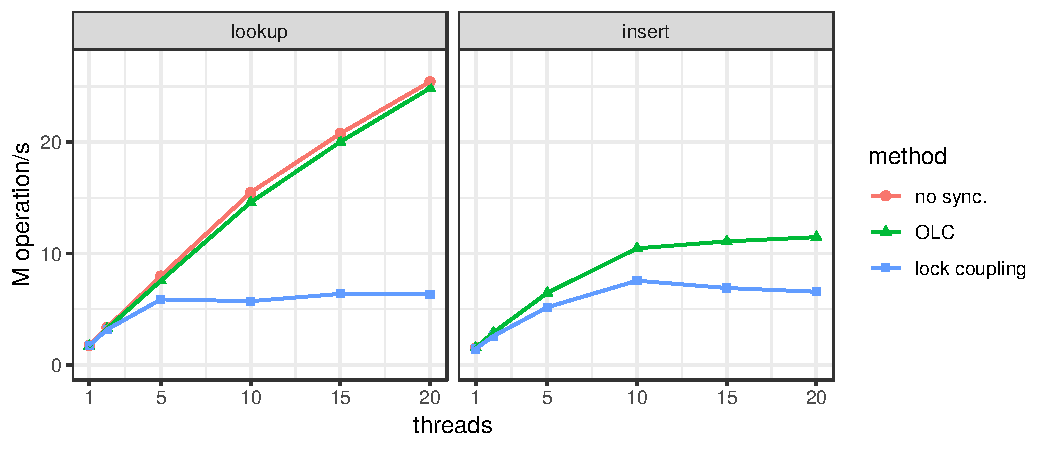
\includegraphics[width=\linewidth]{scale.pdf}
  \vspace{0.2cm}
  \caption{Scalability on 10-core system for B-tree operations (100M values).}
  \label{fig:scale}
\end{figure}

As Figure~\ref{fig:scale} shows, the results change dramatically once we use multiple threads.
For lookup, the scalability of OLC is near-linear up to 20 threads, even though the system has only 10 ``real cores''.
The OLC scalability for insert is also respectable (though not quite as linear because multi-threaded insertion approaches the memory bandwidth of our processor).
The figure also shows that the results of traditional lock coupling with read/write locks are significantly worse than OLC.
With 20 threads, lookup with OLC is 3.9$\times$ faster than traditional lock coupling.

\section{Summary}\label{sec:conc}

Optimistic Lock Coupling (OLC) is an effective synchronization method that combines the simplicity of traditional lock coupling with the superior scalability of lock-free approaches.
OLC is widely applicable and has already been successfully used to synchronize several data structures, including B-trees, binary search trees, and different trie variants.
These features make it highly attractive for modern database systems as well as performance-critical systems software in general.

\begin{thebibliography}{10}

\bibitem{DBLP:conf/spaa/BalmauGHZ16}
O.~Balmau, R.~Guerraoui, M.~Herlihy, and I.~Zablotchi.
\newblock Fast and robust memory reclamation for concurrent data structures.
\newblock In {\em SPAA}, 2016.

\bibitem{DBLP:journals/acta/BayerS77}
R.~Bayer and M.~Schkolnick.
\newblock Concurrency of operations on {B}-trees.
\newblock {\em Acta Informatica}, 9, 1977.

\bibitem{hot}
R.~Binna, E.~Zangerle, M.~Pichl, G.~Specht, and V.~Leis.
\newblock {HOT}: A height optimized trie index for main-memory database
  systems.
\newblock In {\em SIGMOD}, 2018.

\bibitem{DBLP:conf/ppopp/BronsonCCO10}
N.~G. Bronson, J.~Casper, H.~Chafi, and K.~Olukotun.
\newblock A practical concurrent binary search tree.
\newblock In {\em PPOPP}, 2010.

\bibitem{DBLP:conf/vldb/ChaHKK01}
S.~K. Cha, S.~Hwang, K.~Kim, and K.~Kwon.
\newblock Cache-conscious concurrency control of main-memory indexes on
  shared-memory multiprocessor systems.
\newblock In {\em VLDB}, 2001.

\bibitem{intel}
I.~Cutress.
\newblock {Intel} goes for 48-cores: {Cascade-AP} with multi-chip package
  coming soon.
\newblock
  \url{https://www.anandtech.com/show/13535/intel-goes-for-48cores-cascade-ap},
  2018 (accessed January, 2019).

\bibitem{DBLP:conf/cidr/FaleiroA17}
J.~M. Faleiro and D.~J. Abadi.
\newblock Latch-free synchronization in database systems: Silver bullet or
  fool's gold?
\newblock In {\em CIDR}, 2017.

\bibitem{DBLP:journals/ftdb/Graefe11}
G.~Graefe.
\newblock Modern {B}-tree techniques.
\newblock {\em Foundations and Trends in Databases}, 3(4), 2011.

\bibitem{DBLP:conf/hpca/KarnagelDRLLSL14}
T.~Karnagel, R.~Dementiev, R.~Rajwar, K.~Lai, T.~Legler, B.~Schlegel, and
  W.~Lehner.
\newblock Improving in-memory database index performance with
  {Intel}\({}^{\mbox{{\textregistered}}}\) transactional synchronization
  extensions.
\newblock In {\em HPCA}, 2014.

\bibitem{DBLP:journals/tods/LehmanY81}
P.~L. Lehman and S.~B. Yao.
\newblock Efficient locking for concurrent operations on {B}-trees.
\newblock {\em {ACM} Trans. Database Syst.}, 6(4), 1981.

\bibitem{leanstore}
V.~Leis, M.~Haubenschild, A.~Kemper, and T.~Neumann.
\newblock Leanstore: In-memory data management beyond main memory.
\newblock In {\em ICDE}, 2018.

\bibitem{art}
V.~Leis, A.~Kemper, and T.~Neumann.
\newblock The adaptive radix tree: {ARTful} indexing for main-memory databases.
\newblock In {\em ICDE}, 2013.

\bibitem{htmtkde}
V.~Leis, A.~Kemper, and T.~Neumann.
\newblock Scaling {HTM}-supported database transactions to many cores.
\newblock {\em {IEEE} Trans. Knowl. Data Eng.}, 28(2), 2016.

\bibitem{artsync}
V.~Leis, F.~Scheibner, A.~Kemper, and T.~Neumann.
\newblock The {ART} of practical synchronization.
\newblock In {\em DaMoN}, 2016.

\bibitem{DBLP:conf/icde/LevandoskiLS13a}
J.~J. Levandoski, D.~B. Lomet, and S.~Sengupta.
\newblock The {Bw}-tree: A {B}-tree for new hardware platforms.
\newblock In {\em ICDE}, 2013.

\bibitem{DBLP:journals/pvldb/MakreshanskiLS15}
D.~Makreshanski, J.~J. Levandoski, and R.~Stutsman.
\newblock To lock, swap, or elide: On the interplay of hardware transactional
  memory and lock-free indexing.
\newblock {\em {PVLDB}}, 8(11), 2015.

\bibitem{DBLP:dblp_conf/eurosys/MaoKM12}
Y.~Mao, E.~Kohler, and R.~T. Morris.
\newblock Cache craftiness for fast multicore key-value storage.
\newblock In {\em EuroSys}, 2012.

\bibitem{DBLP:journals/tpds/Michael04}
M.~M. Michael.
\newblock Hazard pointers: Safe memory reclamation for lock-free objects.
\newblock {\em {IEEE} Trans. Parallel Distrib. Syst.}, 15(6), 2004.

\bibitem{DBLP:journals/jacm/ShalevS06}
O.~Shalev and N.~Shavit.
\newblock Split-ordered lists: Lock-free extensible hash tables.
\newblock {\em J. {ACM}}, 53(3), 2006.

\bibitem{amd}
A.~Shilov.
\newblock {AMD} previews {EPYC} ‘{Rome}’ processor: Up to 64 {Zen} 2 cores.
\newblock
  \url{https://www.anandtech.com/show/13561/amd-previews-epyc-rome-processor-up-to-64-zen-2-cores},
  2018 (accessed January, 2019).

\bibitem{DBLP:conf/sosp/TuZKLM13}
S.~Tu, W.~Zheng, E.~Kohler, B.~Liskov, and S.~Madden.
\newblock Speedy transactions in multicore in-memory databases.
\newblock In {\em SOSP}, 2013.

\bibitem{buzzword}
Z.~Wang, A.~Pavlo, H.~Lim, V.~Leis, H.~Zhang, M.~Kaminsky, and D.~Andersen.
\newblock Building a {Bw}-tree takes more than just buzz words.
\newblock In {\em SIGMOD}, 2018.

\end{thebibliography}


%\bibliographystyle{abbrv}
%\bibliography{main}

\end{document}

\end{article}



\end{articlesection}

% put the news items below- there can be multiple news sections
% each with its own title
% news will usually have an author as well as a title, 
% e.g. TCDE elections
% news articles are in the same format as letters
% typically, news articles will be stored in a directory called "news"

%\begin{newssection}{News headline}

% insert news items here; news will typically have authors
% see the Sept. 2018 issue for an example

%\begin{news}{news item title}
%{author name}{author affiliation}
%\input{news/news-article.tex}
%\end{news}
%
%\newpage


%\end{newssection}

\begin{awardsection}
\begin{award}{Letter from the Impact Award Winner}
{Christian S. Jensen}{Aalborg University, Denmark}
\documentclass[11pt]{article}
\usepackage{deauthor,times}

\begin{document}

%\noindent
%\textbf{\Large Letter from the 2019 IEEE TCDE Impact Award Winner}
%\newline

% \title{Letter from the 2019 IEEE TCDE Impact Award Winner}
% \maketitle
I was very happy and humbled to receive this year's TCDE Impact Award, with the citation ``for contributions to spatial, temporal, and spatio-temporal data
management.'' I would like to thank those who nominated me as well as the awards'd committee. Conducting research is very much a social, or collaborative, activity, and I have worked with many excellent colleagues on the three topics mentioned in the citation, and they deserve most of the credit for the results that I have contributed to achieving. I will mention some of them as I cover aspects of my research journey. I started out working on temporal databases and then later transitioned to working on spatial and spatio-temporal databases. To achieve some degree of brevity, I will offer an account of only some of the activities related to temporal data management. I thus start at the very beginning of my academic life.

\paragraph{The Early Years---Ph.D.\ Studies} I received my M.Sc.\ degree in computer science from Aalborg University in 1988.  At that time, the M.Sc.\ study had a formal duration of five and a half years and included two B.Sc.\ degrees (in my case, in Mathematics and Computer Science). The last half year was devoted to the M.Sc.\ thesis, but the mindset at the time was that you were not serious if you spent less than a year. Thus, having received the M.Sc.\ degree after six years of study, I received a scholarship to go and study for a Ph.D.\ for two and a half years anywhere in the world. All I needed to do was to write a thesis---the course requirements were already satisfied.

In early September 1988, I then arrived at Dulles Airport. My M.Sc.\ supervisor, Lars Mathiassen, now a professor at Georgia State University, had recommended that I study under the direction of Leo Mark, then a young faculty member at the University of Maryland. I still remember driving with Leo from Dulles to his house in the late evening with all the windows open in his (by Danish standards) huge and very American Chevy. An exciting journey had started.

A November 25, 1988 plan gave the following working title for my thesis: ``A By-Relation Implemented Object Oriented Data Model Supporting Efficient Storage and Retrieval of Versions of Complex Objects in Engineering Applications.'' I started out looking at the versioning aspect, and this led to studies of support for transaction time, which I viewed as an ideal foundation for fine-grained version support. The eventual title of the thesis was ``Towards the Realization of Transaction Time Database Systems,'' and I had become interested in temporal databases.

\paragraph{The Pursuit of Industrial Impact} Having completed the Ph.D.\ studies and defended the thesis back in Denmark in January 1991, I packed up my car in Greenbelt, MD and drove cross-country to Tucson, AZ, where I was to work with the most visible temporal database researcher, Rick Snodgrass, then a young faculty member at the University of Arizona. I had received a faculty position at Aalborg University that allowed me to spend my first semester with Rick. Our interests matched very well, and we got off to a very good start. This turned into three more sabbaticals, in 1992, 1994, and 1999, where I also got the opportunity to work with Rick's students, Curtis Dyreson, Nick Kline, and Mike Soo.

The 1990s were exciting times in temporal databases. The field had witnessed a proliferation of temporal data models and query languages, almost to the point of each researcher having their own model and language. It was felt that this blocked industrial impact, and initiatives were taken to achieve a consensus temporal data model and query language. This resulted in the TSQL2 query language, which was designed by an 18-person committee led by Rick. 

Pursuing the goal of achieving industrial impact, Rick subsequently was the main force behind attempts to standardize TSQL2. This turned out to be a difficult process, in part due to politics and a variety of interests, but we also made technical progress. Specifically, we learned that the TSQL2 design approach did not scale well: Adding support for some temporal functionality to SQL worked fine, but adding comprehensive support following the TSQL2 approach was not pretty. While SQL is not a pretty language in the first place in terms of design, the TSQL2 approach yielded a result that was uglier than we would have liked. Something different was needed. As we were making these revelations, Michael B\"{o}hlen joined the University of Arizona as a postdoc. He had worked on an approach to language design that inspired the introduction of so-called statement modifiers into TSLQ2. The idea is that many temporal queries can be expressed intuitively and unambiguously as a single-state, non-temporal (and easy-to-formulate) SQL query that is then performed, as specified by a statement modifier, on all states of a temporal relation, after which the results are combined into a temporal relation. So a temporal query could then be formulated by a non-temporal query prefixed by some modifiers. A careful design based on this approach was introduced into standards proposals, and an ``academic'' version called ATSQL was also designed and documented in a TODS 2000 paper titled ``Temporal Statement Modifiers.''

In parallel with the above, I also worked on a range of other subjects in temporal databases, including database design, covering logical and conceptual temporal database design; data model and query language design aspects; support for the notion of ``now'' and for data aging; indexing; implementation of temporal algebra operators; query optimization; and architectures for implementing temporal query language support. I worked with five of my first six Ph.D.\ students on these topics: Kristian Torp, Heidi Gregersen, Dieter Pfoser, Janne Skyt, and Giedrius Slivinskas.

\paragraph{The Recent Years} While spatial and spatio-temporal databases started to take over as my main activity around year 2000, I have continued to maintain an interest in temporal databases. Following his postdoc at Arizona, Mike joined the faculty at Aalborg University. He later moved to the Free University of Bozen-Bolzano and he is now back home in Switzerland, at the University of Zurich. I have been fortunate to be able to continue to work on temporal databases with Mike, Hans Gamper from Bolzano, and most recently Anton Dign\"{o}s, as a Ph.D.\ student at Zurich and now as a faculty member at Bolzano. A key goal was to achieve an implementation of ATSQL. With other colleagues, we looked at many options, but it took until 2016, i.e., 16 years, before we had solid results. In particular, Anton's Ph.D.\ thesis and a TODS 2016 paper titled ``Extending the Kernel of a Relational DBMS with Comprehensive Support for Sequenced Temporal Queries'' show how to extend the kernel of PosgreSQL to enable efficient support for the functionality described in the TODS 2000 paper.

\paragraph{Impact and Lessons} Looking back, one may ask what the impact of this work has been. Certainly, the literature suggests that the work has influenced other research in the field, but there has also been impact beyond academia. One highlight is that Teradata put temporal support into their system based on the statement modifier approach, which made them a pioneer in offering temporal support. This was done before ANSI/ISO standardization. Today, Teradata in addition supports the temporal tables and (limited) query language syntax in the standard. Another highlight is that the PostgreSQL implementation described in the TODS 2016 paper is available for anyone to use. A different line of impact is in the area of database design, where national statistics bureaus (e.g., Statistics Denmark) and archives (e.g., Danish National Archives) make use of temporal tables, including bi-temporal tables, when organizing their data. I have been contacted by, and have interacted with, several such entities. While the standards have adopted a language design approach that I think does not scale, and while there is a disconnect between SQL standardization and academia, I do believe that the standard is influenced by advances in temporal database research. For example, the standard supports bitemporal tables: We studied such tables in depth and even coined the term bitemporal.

Finally, I want to make a few points. First, research is often a social and collaborative effort. One should try to work with good colleagues (check!) and try to be a good colleague. Second, it can take decades to achieve societal impact, which is at odds with the increasing dependence on short externally funded projects in order to be able to perform research. Third, the disconnect between stardardization and academia is unfortunate from a societal perspective. Fourth, in research, one often does not quite know where one ends when starting.

%\begin{flushright}
%Christian S.\ Jensen\\
%Aalborg University  
%\end{flushright}

\end{document}

\end{award}
\newpage
\begin{award}{Letter from the Service Award Winner}
{David Lomet}{Microsoft Research, USA}
\documentclass[11pt]{article} 

\usepackage{deauthor,times,graphicx}
%\usepackage{url}
\usepackage{hyperref}

\begin{document}

\section*{Icing on the Cake}

I have had the honor and pleasure of serving for 25+ years and over 100 issues as the Editor-in-Chief (EIC) of the Data Engineering Bulletin, the very publication in which this letter is being published.  I never dreamed, while pondering the Bulletin EIC offer from Rakesh Agrawal, then the TCDE chair in 1992, that I would make the Bulletin so significant a part of my career.  To now get rewarded with the TCDE Service Award is truly ``icing on the cake''.  I am thankful to the TCDE both for the opportunity to serve as Bulletin EIC and now for being honored for this service with this award.

The Bulletin has been such a large part of my technical career and my primary service activity until just recently, when I have become 
involved with Computer Society governance.  And the beauty of how this all worked out is that the Bulletin has truly been a ``labor of love''.  Where else can database professionals learn what is happening in a subarea of our field, brought together in a single issue, with contributions from research and industrial leaders.  

In the database area, which changes so fast, the ability of the Bulletin to provide a special issue on a new topic is both unique and invaluable.  The ability of Bulletin editors to bring leading technologists together to write articles for an issue is the ``magic sauce'' that makes the entire enterprise a success.  Over the years, it has been my pleasure to work with so many of the gifted editors whose work you see in every issue published.  I like to think that I also contributed to the success of the Bulletin-- but my success was one level indirect.  It was my success over the years of convincing distinguished members of the database community to serve as Bulletin editors.  As one mark of this success, the editors I have appointed include seven Codd Award winners, all but one prior to their receiving the award.  And I have no doubt there will be more winners in the future.

The Bulletin would not exist without articles written by so many distingushed members of our database community.  Their willingness to contribute articles is a direct result of you, our readers, who so eagerly consume Bulletin articles.  The result of this is a virtuous cycle: distinguished editors attract distinguished authors, who write articles that are read and cited by many members of our database community.  So you, dear reader, have played an essential role in making this system work. 

Over the years, the Bulletin has transformed from solely paper publication to a mixed paper-electronic publication to finally an entirely electronic publication.  Over that time, my job at Digital Equipment Corp. (DEC) transformed into a job at Microsoft.  My thanks to both employers, who so generously permitted me to spend time on the Bulletin for so many years, and who provided the initial web infrastructure that made the Bulletin available electronically.

Haixun Wang, my successor and current Bulletin EIC, now has three issues "under his belt".  So the future of the Bulletin looks very promising.  He has recently introduced an "opinion" section, and asked me to contribute an opinion piece in the first issue with the new section.  This was my first non-letter Bulletin publication since 1987 (before I became EIC).  I am hoping it is not the last as, like so many others in our community, I value the Bulletin as a channel for publishing my technical contributions.
 
And now, finally, I too have the pleasure of reading Bulletin articles-- focusing on their technical content, rather than being concerned (and consumed) by formatting and editorial issues.  I have already begun enjoying this post-EIC role, and look forward to this continuing.  Thank you all for contributing to the success of the Bulletin and for making my involvement so personally gratifying.

\end{document}



\end{award}
\newpage
\begin{award}{Letter from the Rising Star Award Winner}
{Viktor Leis}{Friedrich-Schiller-Universität Jena}
\pdfminorversion=5
\documentclass[11pt]{article}
\usepackage{deauthor,times,graphicx,caption,microtype}

\begin{document}

%\section*{Letter from the 2019 IEEE TCDE Early Career Award Winner}

I am honored to have received the 2019 IEEE TCDE Early Career Award ``for contributions to main-memory indexing and database architectures for NVM''.
Let me use the opportunity of this letter to describe three open, interrelated problems in this area that I consider both interesting and important.

\subsubsection*{Is the current dominance of LSM trees over B-tree justified?}

For decades, virtually all database systems relied on B-trees for indexing (with hashing being a distant second).
Most modern NoSQL, NewSQL, and cloud database systems, in contrast, primarily rely on Log-Structured Merge-trees (LSM) as their main data structure.
B-trees and LSMs differ in terms of many different dimensions: in-place vs.~out-of-place writes, eager writes vs.~background merges, favoring reads vs.~writes, etc.
I therefore wonder: Have B-trees become obsolete? Are LSMs just a fad? Is it possible to design a data structure that combines the best properties of the two approaches?

\subsubsection*{Do we need a new class of database systems for flash arrays?}

In the past 7 years, main memory capacities have stagnated.
The first commercially-available version of byte-addressable non-volatile memory (``Intel Optane DC Persistent Memory'') turned out to be as expensive as DRAM, but significantly slower.
Flash, on the other hand, has become much cheaper during this time frame and is now 20$\times$ cheaper than DRAM per byte.
Furthermore, flash has become much faster, and it is now possible to directly attach a dozen or more devices to a single server, which results in a theoretical aggregated bandwidth close to DRAM.
Neither traditional disk-based, nor modern in-memory or NVM-based database systems are capable of exploiting such extremely fast flash devices.
This raises the question of whether a new system design is needed and how it would differ from existing approaches.

\subsubsection*{How to exploit hardware fluidity in the cloud?}

When developing high-performance database systems, most of us implicitly assume that the hardware is fixed and optimize for a particular configuration.
Given how most organizations procure hardware, this a reasonable approach.
In the cloud, however, because it is easy to migrate to a different instance with potentially very different underlying properties, hardware should not be thought of as fixed.
After all, users care about performance and cost, not about which kind of instances their service runs on.
Therefore, cloud-native database systems could autonomously optimize the hardware configuration they run on.
This requires an economical, literally cost-based approach that takes actual market prices into account.

%\begin{flushright}
%Viktor Leis\\
%Friedrich-Schiller-Universit\"at Jena
%\end{flushright}

\end{document}

\end{award}
\end{awardsection}



\begin{callsection}

%  This section will be empty for your version
%
%  Calls for papers section.  Use the callsection environment.
%  Each call for papers is contained in an call environment, where the single 
%  required options to \begin{call} is the name of the conference.
% typically calls are stored in a "calls" directory
%
%\begin{call}{name of conference}
%\centerline{\includegraphics[width=\textwidth, bb= 0 0 590 760]{calls/conference-name.pdf}}
%\end{call}
%\begin{call}{ICDE 2019 Conference}
%\centerline{
\includegraphics[width=\textwidth, bb= 0 0 610 790] {../Dec-2018/calls/icde19.pdf}} 
%\centerline{
\includegraphics[width=\textwidth, bb= 0 0 590 760] {calls/icde19.pdf}}
%\end{call}
\begin{call}{TCDE Membership Form}
%\centerline{\includegraphics[width=\textwidth, bb= 0 0 610 790]
\centerline{
\includegraphics[width=\textwidth, bb= 0 0 590 760] {../Dec-2018/calls/tcde.pdf}}
\end{call}

\end{callsection}

\end{bulletin}
\end{document}
